\documentclass[11pt,a4j,dvipdfmx, twoside]{jreport}

\usepackage{comment}
\usepackage{float}
\usepackage{color}
\usepackage{multicol}
\usepackage{multirow}
\usepackage[dvipdfmx]{pict2e}
\usepackage{wrapfig}
\usepackage{graphicx}
\usepackage{bm}
\usepackage{url}
\usepackage{underscore}
\usepackage{colortbl}
\usepackage{tabularx}
\usepackage{fancyhdr}
\usepackage{ulem}
\usepackage{cite}
\usepackage{amsmath,amssymb,amsfonts}
\usepackage{algorithmic}
\usepackage{textcomp}
\usepackage{xcolor}
\usepackage[ipaex]{pxchfon}
\usepackage{pdfpages}
\usepackage{subcaption}
\usepackage{array}
\usepackage{adjustbox}
\usepackage{lipsum}

\usepackage[number-unit-product=~]{siunitx}

\usepackage[top=30truemm,bottom=30truemm,left=25truemm,right=25truemm]{geometry}

\renewcommand{\arraystretch}{1.2}
\usepackage{docmute}
% プリアンブル部分にインプットしてください。
\newcommand{\ifdraft}{false}

%=======================================================================

\begin{document}

%=======================================================================

\documentclass[11pt,a4j]{jreport}

\usepackage{comment}
\usepackage{float}
\usepackage{color}
\usepackage{multicol}
\usepackage{multirow}
\usepackage[dvipdfmx]{pict2e}
\usepackage{wrapfig}
\usepackage{graphicx}
\usepackage{bm}
\usepackage{url}
\usepackage{underscore}
\usepackage{colortbl}
\usepackage{tabularx}
\usepackage{fancyhdr}
\usepackage{ulem}
\usepackage{cite}
\usepackage{amsmath,amssymb,amsfonts}
\usepackage{algorithmic}
\usepackage{textcomp}
\usepackage{xcolor}
\usepackage[ipaex]{pxchfon}
\usepackage{pdfpages}
\usepackage{subcaption}
\usepackage{array}
\usepackage{adjustbox}
\usepackage{lipsum}

\usepackage[number-unit-product=~]{siunitx}

\usepackage[top=30truemm,bottom=30truemm,left=25truemm,right=25truemm]{geometry}

\renewcommand{\arraystretch}{1.2}

\begin{document}

\thispagestyle{empty}

\begin{center}
  \vspace{20mm}
  {\Large\noindent\textbf{東京大学大学院工学系研究科}}\\
  \medskip
  {\Large\noindent\textbf{建築学専攻}}\\
  \vspace{30mm}
  {\Large\noindent\textbf{2023年度}}\\
  \medskip
  {\huge\noindent\textbf{修 士 論 文}}\\
  \vspace{30mm}
  {\huge\noindent{反射音到来方向が合唱者に}}\\
  \medskip
  {\huge\noindent{与える影響に関する実験的検討}}\\
  \vspace{70mm}

  {\Large\noindent
  2024年1月15日 提出\\
  2024年2月28日 修正\\
  指導教員 佐久間 哲哉 教授    \\
  \vspace{\baselineskip}
  学籍番号 37-226077 \\
  \vspace{\baselineskip}
  板垣 大稀\\
  }
  \vspace{40mm}

\end{center}

\thispagestyle{empty}
\clearpage

\end{document}

%=======================================================================
% \renewcommand{\abstractname}{要旨}


%=======================================================================

% 目次の表示
\tableofcontents


%=======================================================================
\pagestyle{fancy}
\rhead{\rightmark}
\lhead{\leftmark}
\renewcommand{\chaptermark}[1]{\markboth{第\ \normalfont\thechapter\ 章~~#1}{}}
%=======================================================================
\cleardoublepage
\documentclass[11pt,a4j]{jreport}

\usepackage{comment}
\usepackage{float}
\usepackage{color}
\usepackage{multicol}
\usepackage{multirow}
\usepackage[dvipdfmx]{pict2e}
\usepackage{wrapfig}
\usepackage{graphicx}
\usepackage{bm}
\usepackage{url}
\usepackage{underscore}
\usepackage{colortbl}
\usepackage{tabularx}
\usepackage{fancyhdr}
\usepackage{ulem}
\usepackage{cite}
\usepackage{amsmath,amssymb,amsfonts}
\usepackage{algorithmic}
\usepackage{textcomp}
\usepackage{xcolor}
\usepackage[ipaex]{pxchfon}
\usepackage{pdfpages}
\usepackage{subcaption}
\usepackage{array}
\usepackage{adjustbox}
\usepackage{lipsum}

\usepackage[number-unit-product=~]{siunitx}

\usepackage[top=30truemm,bottom=30truemm,left=25truemm,right=25truemm]{geometry}

\renewcommand{\arraystretch}{1.2}

\begin{document}

\chapter{はじめに}
%=====================================================================

\section{背景} %1.1
本研究は反射音の到来方向が演奏者に与える影響について検討を行うものであり、コンサートホール音響学の中でも特に演奏者の立場からホールの評価を行うことを試みるステージ音響学の分野に位置づく。研究の前史として、まずコンサートホールの起源とその研究の起こりについて概観する。

\subsection*{コンサートホールの起源}
18世紀以前のヨーロッパにおいて音楽家は主に王室や貴族、教会の保護下で活動していたが、18世紀後半になるとブルジョワジーと呼ばれる中産階級が社会の富と実験を握り始めたことで従来の庇護者の力が相対的に弱まり、市民層を対象としたコンサートにより収入を得る音楽家が現れたとされる。

最初期のコンサートホールは既存の建物を利用したものだったが、市民向けコンサートが興行的な成功を収めるようになると、より多くの聴衆を収容する必要性が高まり、コンサート用の会場として約800席の座席数を持つハノーヴァー・スクエア・ルームズ(1774年)などが建設されるようになった。19世紀以降には2000席程度の座席数を誇るようなより大規模なコンサート専用ホールがヨーロッパ各地に建設されるようになり、特に代表的な初期の大規模コンサートホールとして、ウィーン楽友協会大ホール (1870)、初代ベルリン・フィルハーモニー (1882)、アムステルダムのコンセルトヘボウ (1888)が挙げられる。ルネサンス期に成立したオペラのための大規模な劇場は18世紀にはヨーロッパ各地に建造されていたことを思うと、コンサートホールの歴史は比較的新しいものと言えよう。

\vspace{1\baselineskip}

\begin{figure}[H]
  \begin{minipage}[t]{0.5\linewidth}
    \centering
    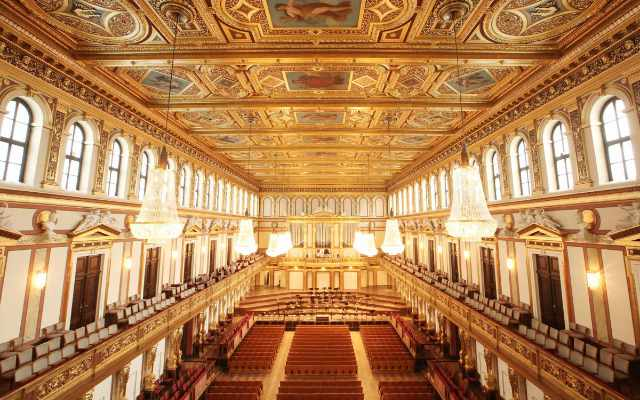
\includegraphics[width=0.9\linewidth]{images/pictureCitation/resized/musikverein.jpg}
    \caption{ウィーン楽友協会大ホール}
    \footnotesize © Wolf-Dieter Grabner, ウィーン楽友協会\\公式ホームページ \cite{musikverein}
    \label{fig:ウィーン楽友協会大ホール}
  \end{minipage}%
  \begin{minipage}[t]{0.5\linewidth}
    \centering
    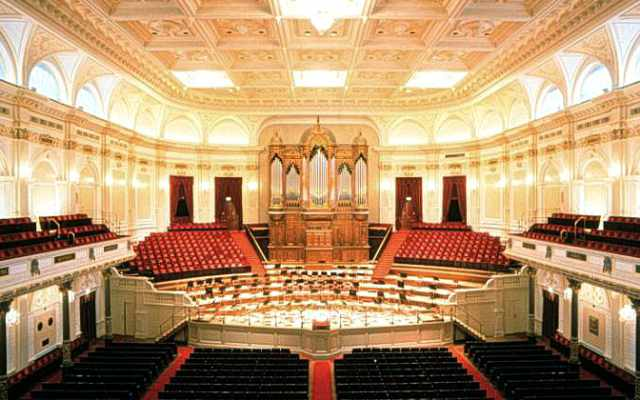
\includegraphics[width=0.9\linewidth]{images/pictureCitation/resized/Concertgebouw.jpg}
    \caption{アムステルダム コンセルトヘボウ}
    \label{fig:コンセルトヘボウ}
    \footnotesize © Amsterdam Municipal Department for the\\ Preservation and Restoration of Historic\\ Buildings and Sites (bMA) \cite{Concertgebouw}
  \end{minipage}
\end{figure}

%=====================================================================

\newpage
\subsection*{コンサートホール音響学の創始}

これらのホールは靴箱のような直方体の空間形状からシューボックス型と呼ばれる形式で、この形状がコンサートホールの形として良いのではないかということは経験的に認識されていたという。特にウィーン楽友協会大ホールは響きの優れたホールとしても有名であるが、しかし、これらのホールの響きは必ずしも音響設計によって狙った響きが実現されたものではない。コンサートホールの建造にあたっての本格的な音響設計の開始は、ボストンシンフォニーホールの設計におけるSabineの音響コンサルティングを待つことになる\cite{清水寧2023}。

Sabineはハーバード大学の物理学の研究者であり、彼の建築音響に関する研究はハーバード大学に建設された Fogg Art Museum (1895)の講義室に生じた「残響により言葉が明瞭に聞こえない」という音響的な問題の改善を依頼されたことから始まった。この問題の解決のための過程でSabineが導入した残響時間や吸音率といった概念は現代の室内音響学の基礎となっており、ボストンシンフォニーホールの音響設計においてもこれらの概念を活用して設計が進められた。これらのSabineの取り組みにより、建築音響工学、そしてコンサートホール音響学が創始された\cite{sabine2005}。それ以降、優れた音響空間をいかにして建築するかという課題に向かって、基本的な残響感から極めて感性的な判断である音の好みに至るまで、物理的あるいは聴覚心理的視点から数多くの研究が積み重ねられてきた。

\vspace{1\baselineskip}

\begin{figure}[H]
  \centering
  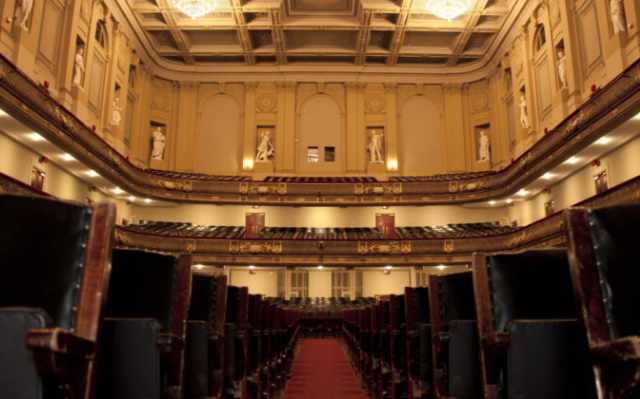
\includegraphics[width=.45\linewidth]{images/pictureCitation/resized/bostonSymphony.jpg}
  \caption{ボストン シンフォニーホール}
  \label{fig:ボストンシンフォニーホール}
  \footnotesize ボストンシンフォニーホール公式ホームページより \cite{bostonSymphony}
\end{figure}

%=====================================================================
\newpage
\section{既往研究}

\subsection*{ステージ音響学の始まり}
演奏者にとっても空間の響きが極めて重要であることは演奏者にとっては半ば自明であって、ホール設計者や音響学の研究者にもよく知られていたのではないかと推測されるが、コンサートホール音響学に関する研究は、主に客席での聴こえ方、すなわち聴衆の視点に立って行われてきた。演奏者の視点に立ったコンサートホールに関する音響学の研究領域は今日では「ステージ音響学」と呼ばれて分類されるが、この研究が本格的に行われるようになるのは1970年代に入ってからのことである。

ステージ音響の研究がSabineによるコンサートホール音響学の創始から随分と遅れて始まった理由を直接述べることは困難であるが、「演奏家はホールを評価するというよりも、どうしたらそのホールで良い演奏ができるかということを考える」という言葉\cite{橘1997}によく表れてように、熟練した演奏者であれば空間の響きに合わせて演奏を適応させるべきであると他ならぬ演奏者自身が考えているであろうという動機の点は一つの理由として考えられる。またこのような適応的な演奏の変化を行うという事実から、多数の演奏者を対象として信頼性の高い均一な主観評価結果を得るのが難しいという研究上の困難さがある点も、その理由の一部ではないかと推測できる。
  
ともかくコンサートホール音響学の創始から遅れつつも1970年代にステージ音響に関する研究は始まり、その初期の研究は、模擬音場での演奏実験によって\cite{marhsall1978, nakayama1984, naylor1988}、または実際のホールステージの現場での実験によって\cite{Gade1989II, chiang2003, jeon2005}、音場に対する演奏者の主観印象の評価を求めるものであった。

さらに、菅\cite{suga1986}は演奏者が好むステージ音響状態を説明する指標として「響きの量」「響きの質」「自分の音の出しやすさ」「自分の音の聞き取りやすさ」「他の演奏の聞き取りやすさ」「音の鳴りの手応え」「弱音の伸び」「音の通り」のそれぞれの関係を検討している。その結果、ホールの音響的印象は響きの量・質、自分の音の出しやすさ、聞き取りやすさの四要因の評価でほとんど決定されること、演奏のしやすさの評価はこのうち前三者との相関が高く、これらが音響的総合印象を支配する要因であるとしている。

舞台音響特性の物理的な測定を通した大規模な調査は1989年にGade\cite{Gade1989II}によって初めて行われ、演奏者自身の演奏のしやすさに関する物理指標値として”SUPPORT(ST)”、アンサンブルの取りやすさに関する指標値として”Early Ensemble Level(EEL)”が定義された。また、指揮者、歌手、オーケストラ団員に対するインタビューを通し、演奏家のホールに対する評価項目を響き(Reverberance)、自分の音の聞きやすさ(Support)、音色(Timbre)、ダイナミクス(Dynamics)、互いの音の聞きやすさ(Hearing Each Other)、時差(Time Delay)の六つにまとめている。これらGadeの取り組みの成果がステージ音響学が本格化する画期となったと考えられ、今日ISO3382-1:2009にもSTおよびEELが規格化されており、音響設計やステージ音場の評価に用いられている。なお、ステージ音響指標STに関する説明について、またGadeの提案からISOに規格化されるまでのステージ音響指標値に関する研究の経緯については第2章第1節にて詳細に記述する。

\newpage
\subsection*{ステージ音響学の発展}

菅ら\cite{suga1995}はボストン交響楽団、ライプツィヒ・ゲヴァンドハウス管弦楽団、新日本フィルハーモニー交響楽団の団員に対して多数のホールでのコンサートに基づく主観評価調査を行った結果からホールの音響設計という観点から考慮すべき点について考察し、「舞台の大きさ」「舞台音響反射板の開き具合」「舞台音響反射板の拡散性」という三点をまとめている。

上野ら\cite{Ueno2003a}は、演奏家のホールに対する心象が演奏という能動的行為における個々の意識に密接に関係するものであるため、ホールに対する演奏家の意識の理解のために、実験により検証可能な仮説を設定して統計的にその妥当性を確かめる一般的な心理統計的手法を適用することが難しいという問題を指摘した上で、ホールの音響効果に関する演奏家の言語構造について検討を行い、その結果として、演奏中の演奏家の意識に関して「個人」「共演者」「聴衆」の三つの軸を想定することにより演奏家の言語表現が整理された。

上野らはさらに、演奏者がホール音場についてどのように考えているかについて、演奏者自身の言葉を用いて個人別の評価項目を作成して評価を行う"個別尺度法"を適用した主観評価実験を行い、各演奏家の好みなど総合的な評価に関しては個人差が大きく表れるのに対し、具体的な響きの特徴や音の聴こえ方については複数の演奏家がある程度共通した判断を行っていることを報告している\cite{Ueno2003a}。


\subsection*{ステージへの反射音の到来方向に関する研究}
Gadeにより提案され、今日ではISOに規格化されるステージ音響指標STおよびEELは、舞台上に音源・受音点を置いて測定したインパルス応答において、直接音のエネルギーに対する反射音のエネルギーの量を評価することで、演奏者の聴取する響きを定量化することを試みる量である。すなわちこれらの音響指標値は、演奏者の聴取する響きのある時間窓の中のエネルギー量に着目して構築された指標であるが、演奏者による響きの評価はその他にも多様な項目により決定されると考えられる。

反射音の到来方向も演奏者の感じる響きの印象に影響を与えうる物理的要因と考えられたもののうちの一つであり、1993年の中村による研究{中村1993}にて演奏者が室の響きの方向性に何らかの影響を受けている可能性が指摘されている。2008年の上田による研究\cite{上田2008}では、6chスピーカーシステムを用いて生成した音場において、反射音の到来方向が左右に偏りがある音場か、後方から多い音場が好まれる可能性があることが示されている。一方で、同じ研究グループにより指摘されているように、実際のステージ上において、このような響きの方向特性に近い音場が実現されていると考えられる舞台側壁または後壁付近を選んで演奏者が演奏を行うことは通常なく、標準的な演奏位置である舞台中央・前方付近では左右の偏り、後方からの反射音供給量ともに比較的小さい\cite{林2008}。

このように、6chスピーカーシステムによる模擬音場での主観評価実験の結果と、現実の音場の響きの条件に関する対応関係は明らかになっていない。方向特性が演奏者に与える影響についてより適切な評価結果を得るためには、より現実に即した音場条件において反射音の到来方向特性を変化させて主観評価実験を行う必要があると考えられるが、このような検討例は見られない。


%=====================================================================

\newpage
\section{本研究の目的} %1.3
ステージ音響における主観評価実験の手法は模擬音場を実験室内に生成して演奏実験を行う方法(6-9,8?)、実際のホールステージの現場にて演奏実験を行う方法(10-13)に大別される。前者は音場要因の制御は後者に比べて容易であるという利点があるが、6chスピーカーシステムをはじめとする従来の手法により生成される模擬音場では、音場領域が狭く現実のホールと同等の測定を行うことが困難であり、生成した音場の特性と現実のホールとの対応関係を明らかにすることが難しい。逆に、実際のホールステージで演奏実験を行おうとする場合、当然のことながら、響きの条件を自由に制御することはほとんど不可能である。

しかし、前項にて現実に即した音場条件での評価の必要性を指摘したように、反射音到来方向が演奏者に与える影響に関する評価のためには、実験環境と現実のコンサートホールステージの間での乖離を可能な限り小さくし、より現実の演奏環境に即した実験を行うことが望ましい。そこで本研究では、実際のコンサートホールの反射音到来方向を模した音場を実験室において生成し、その生成した音場における演奏実験を通して反射音到来方向が演奏者に与える影響について検討することを目的とする。

なお、本研究ではより現実に即した演奏条件下で実験を行うことを試みるため、最も基本的な演奏形態のうちの一つである混声四部のカルテット(ソプラノ、アルト、テノール、バスの四声部各一名ずつからなるアンサンブル形態)にて演奏実験を行うことを考える。

%=====================================================================

\section{AFCの概要} %1.4

本研究では、音場の生成に用いるシステムとして音場支援システム(YAMAHA : Active Field Control Enhance、以下AFC)を採用し、半無響室に導入する。AFCは一つの空間において多様な演目を最適な響きの中で行いたいというモチベーションから開発されたシステムであり、最新の電気音響・信号処理技術を用いて、室内の響きや空間の拡がり・音量感などの聴感印象を自然に変化させることができるシステムである\cite{AFC}。AFCシステムの基本コンセプトを図\ref{fig:AFCシステムの基本コンセプト}に示す。

AFCを用いることによりカルテットによる演奏実験および現実のホールでの測定と同様の音場測定が実施可能なある程度広い範囲に現実に即した自然な音場を生成することが可能であり、また導入する室をもともとの響きのない半無響室とすることで大きな制御幅を得ることが期待できる。

AFCに関する詳細および音場生成の具体的な手法については3章にて記述する。

\lipsum[1-6]
\newpage
\rule{8cm}{6cm}\\
\rule{8cm}{6cm}\\
\rule{8cm}{6cm}

%=====================================================================================
\clearpage
\section{本論文の構成} %1.5
本論文は全5章から構成される。
第1章では、研究背景と反射音到来方向が演奏者に与える影響に関する先行研究について概観し、本研究の目的について述べた。

第2章では、反射音の到来方向について物理的に評価する方法の提案と、その方法によって得られた結果について述べる。

第3章では、第2章では、本研究で用いる音場生成システム、およびそれを導入した実験室のシステム機器構成について述べ、第2章で得られた結果を踏まえて、演奏実験を行う音場を生成する方法について述べる。

第4章では、第3章で得られた音場を用いて行った演奏実験について、その方法、結果および考察について述べる。

第5章では、本研究で得られた整理して総括し、今後の課題について述べる。

\lipsum[1-2]

\newpage
\rule{15cm}{21cm}\\
本論文の構成を示す図

\cleardoublepage

% 参考文献
% 参考文献の箇所にインプットしてください。

% 分割ファイル内でのみ,bibliographyを読み込みます。

\expandafter\ifx\csname ifdraft\endcsname\relax

  % bibliographyを展開する

  \bibliographystyle{junsrt}
  \bibliography{ref.bib}% 同じディレクトリ内のbibファイルのみを参照可能

\fi

\end{document}

%=======================================================================
\cleardoublepage
\documentclass[11pt,a4j]{jreport}

\usepackage{comment}
\usepackage{float}
\usepackage{color}
\usepackage{multicol}
\usepackage{multirow}
\usepackage[dvipdfmx]{pict2e}
\usepackage{wrapfig}
\usepackage{graphicx}
\usepackage{bm}
\usepackage{url}
\usepackage{underscore}
\usepackage{colortbl}
\usepackage{tabularx}
\usepackage{fancyhdr}
\usepackage{ulem}
\usepackage{cite}
\usepackage{amsmath,amssymb,amsfonts}
\usepackage{algorithmic}
\usepackage{textcomp}
\usepackage{xcolor}
\usepackage[ipaex]{pxchfon}
\usepackage{pdfpages}
\usepackage{subcaption}
\usepackage{array}
\usepackage{adjustbox}
\usepackage{lipsum}

\usepackage[number-unit-product=~]{siunitx}

\usepackage[top=30truemm,bottom=30truemm,left=25truemm,right=25truemm]{geometry}

\renewcommand{\arraystretch}{1.2}

\begin{document}

\chapter{反射音到来方向の物理的評価}

%=======================================================================

\section{はじめに}
ステージへの反射音到来方向の物理的評価に関する議論に先立って、ステージ音響学について、特にその指標値が今日用いられるようになるまでの経緯に着目して既往の研究を概観する。

\subsection*{Gadeによるステージ音響指標STの提案}
Gadeは1989年に発表した論文\cite{Gade1989I}の中で、オーケストラ団員に対するインタビューを通して演奏家のホールに対する評価項目を「響き(Reverberance)」「自分の音の聞きやすさ(Support)」「音色(Timbre)」「ダイナミクス(Dynamics)」「互いの音の聞きやすさ(Hearing Each Other)」「時差(Time Delay)」の6つにまとめている。このうち「自分の音の聞きやすさ(Support)」に関して、演奏者自身が発する音に対する初期反射音成分の寄与を評価することを意図し、演奏者に返ってくる音のエネルギーを床からの反射音を含む直接音のエネルギーで基準化してdBで定量化する指標ST(SUPPORT)を考案して、20-100msまたは20-200msの短い時間に到来する反射音を評価する $\mathrm{ST1}$と$\mathrm{ST2}$を式(\ref{eq:ST1})(\ref{eq:ST2})の通り定義した。

\begin{equation}
  \label{eq:ST1}
  \mathrm{ST1}= 10 \log_{10}
  \frac{\int_{20 \: \mathrm{ms}}^{100 \: \mathrm{ms}} p^2(t) dt}
  {\int_{0 \: \mathrm{ms}}^{10 \: \mathrm{ms}} \: p^2(t) \: dt}
\end{equation}

\begin{equation}
  \label{eq:ST2}
  \mathrm{ST2}= 10 \log_{10}
  \frac{\int_{20 \: \mathrm{ms}}^{200 \: \mathrm{ms}} p^2(t) dt}
  {\int_{0 \: \mathrm{ms}}^{10 \: \mathrm{ms}} \: p^2(t) \: dt}
\end{equation}

\vspace{1\baselineskip}

ここで、$p(t)$は音源から舞台後方側に距離$\SI{1.0}{m}$離して設置した無指向性マイクにて測定したインパルス応答を示し、音源および受音点の高さは床から$\SI{1.0}{m}$で、時刻$\SI{0}{ms}$は直接音がマイクに到来した時刻を表す。
  
$\mathrm{ST1}$および$\mathrm{ST2}$の値はステージ上の測定位置によって異なった値を取るが、同時に発表されたこれらの実測を含む研究\cite{Gade1989II}では、典型的なソリストの位置、チェロ奏者の位置、木管楽器の位置の三点がステージの代表点とされた。分析対象の周波数帯域は$\SI{250}{\Hz}$から$\SI{2000}{\Hz}$を中心とする4帯域の1/1オクターブバンドであり、全帯域および全測定点の計算値の算術平均をホールにおける単一の指標値として$\mathrm{ST}$が算出されている。さらに、反射音のエネルギーの大部分は$\mathrm{ST1}$および$\mathrm{ST2}$の評価区間の間に到来するものの、Gadeは同論文にて実施した演奏実験の中で「響き(Reverberance)」および「ダイナミクス(Dynamics)」の評価項目に関して後期反射音が演奏者に与える影響について指摘した上で、これらの評価項目に関わる後期反射音のエネルギーを直接評価する指標として$\mathrm{ST_{Late}}$を式(\ref{STLate})の通り提案している。
  
\begin{equation}
  \label{STLate}
  \mathrm{ST_{Late}}= 10 \log_{10}
  \frac{\int_{100 \: \mathrm{ms}}^{1000 \: \mathrm{ms}} p^2(t) dt}
  {\int_{0 \: \mathrm{ms}}^{10 \: \mathrm{ms}} \: p^2(t) \: dt}
\end{equation}

%=======================================================================

\subsection*{STに関する研究の展開}
前項で示したGadeの研究を嚆矢として、ステージ上での物理的な測定による評価を含む研究がいくつか行われた。

Chiangら\cite{chiang2003}は、舞台面積が$\SI{49}{\m^2}$から$\SI{269}{\m^2}$の範囲で規模の異なる5つのシューボックス型のコンサートホールにおける舞台音響を評価した。各ホールについて、測定位置に関する舞台前方または舞台中央の2条件と側面反射板の有無による2つのステージ条件からなる室内楽を想定した4つの音場条件が検討され、各音場条件について、音源と受音点の位置関係を舞台下手・上手方向または舞台前後方向とする2つの測定位置で測定が行われた。
この研究では$\mathrm{ST2}$は評価せずに$\mathrm{ST1}$を$\mathrm{ST_{Early}}$として呼称が改められて$\mathrm{ST_{Late}}$とともに測定されたほか、比較的小さな舞台寸法を持つホールの壁面から提供される初期反射音のエネルギーを考慮できる$7$〜$\SI{100}{ms}$の積分窓を持つアーリー/ダイレクト・エネルギー比(ED100)も提案された。

JeonとBarron\cite{jeon2005}は、舞台上の位置の違いによる$\mathrm{ST_{Early}}$の値の差異について検討するため、ソウルの扇形平面を持つ大規模なホールのステージ上(舞台面積$\SI{270}{\m^2}$、舞台の幅の平均値$\SI{22}{\m}$、天井の高さ$14$〜$\SI{15}{\m}$)の8つの位置で$\mathrm{ST_{Early}}$の測定を行った。この研究では、音源と受音点の高さとして$\SI{1.2}{\m}$が使用され、これはは演奏者の座位の高さと対応する。測定された$\mathrm{ST_{Early}}$はステージ後方の位置で最も高く、ステージ前方の位置で最も低くなり、その値はそれぞれ約$\SI{-15}{\dB}$、約$\SI{-24}{\dB}$であった。

DammerudとBarron\cite{dammerud2007}は、イギリスの4つのホールのステージで測定と主観的調査を実施した。 舞台面積は$111$~$\SI{189}{\m}$、舞台の幅は$18.0$~$\SI{27.0}{\m}$、平均高さは$9.6$~$\SI{19.0}{\m}$の範囲であった。この研究では、実際の演奏条件を想定してステージ上に椅子が配置された状態にて$\mathrm{ST_{Early}}$および$\mathrm{ST_{Late}}$が測定された。

上野\cite{Ueno2002}は、Gadeが$\mathrm{ST}$の測定において音源と受音点の距離および高さをともに$\SI{1.0}{\m}$としたことに根拠が見られないことを指摘し、演奏家と楽器との関係をモデル化した測定位置として、音源である無指向性スピーカーを楽器の高さを想定した$\SI{1.2}{\m}$、受音点である無指向性マイクを耳の高さを想定した$\SI{1.5}{\m}$とし、音源・受音点の水平面内での中心間距離を楽器と耳の距離を想定した$\SI{0.3}{\m}$の位置とした測定条件においてインパルス応答測定を行ってSTを求めた。その結果、Gadeの測定条件で得られる結果に対して、音源受音点間距離が近いことから、全般的に約7dB程度低い値が得られている。

このように、ステージ音響指標STに関して様々な研究者によって検討がなされてきたが、その一方で測定方法が確立・統一されていないことから、異なる研究機関同士の測定結果を単純に比較して検討することは難しい。Giovannini\cite{giovannini2010}らは主要な楽器セクション間の音響条件の違いを検出することを目的とした測定を行う2008年に投稿した論文の中で、異なる研究者が実施した場合にも比較可能で再現性のある結果が得られるように定義した測定手順について紹介している。

これらの成果はISO3382-1:2009\cite{ISO3382-1}の中にまとめられ、ステージ音響指標$\mathrm{ST_{Early}}$および$\mathrm{ST_{Late}}$が次の式の通りに規格化されている。

\begin{equation}
  \label{eq:STEarly}
  \mathrm{ST_{Early}}= 10 \log_{10}
  \frac{\int_{20 \: \mathrm{ms}}^{100 \: \mathrm{ms}} p^2(t) dt}
  {\int_{0 \: \mathrm{ms}}^{10 \: \mathrm{ms}} \: p^2(t) \: dt}
\end{equation}

\begin{equation}
  \label{eq:STLate}
  \mathrm{ST_{Late}}= 10 \log_{10}
  \frac{\int_{100 \: \mathrm{ms}}^{1000 \: \mathrm{ms}} p^2(t) dt}
  {\int_{0 \: \mathrm{ms}}^{10 \: \mathrm{ms}} \: p^2(t) \: dt}
\end{equation}
%=======================================================================
\newpage
\section{方向別STの提案}
\subsection*{方向別STの定義}
第1章の第2節でも触れたように、反射音の到来方向も演奏者の感じる響きの印象に影響を与えうる物理的要因であることが中村ら\cite{中村1993}により指摘されており、本研究では方向特性が演奏者に与える影響に関して検討を行うことを目的としている。そこで、本研究ではISOに規格化されるSTをもとに方向特性を評価する指標として方向別STを式(\ref{eq:方向別STEarly})および式(\ref{eq:方向別STLate})の通りに構築し、ホールステージの音場の特性の把握および実験室において生成される音場の評価に用いる。

\begin{equation}
  \label{eq:方向別STEarly}
  \mathrm{ST_{Early,dir}}= 10 \log_{10}
  \frac{\int_{20 \: \mathrm{ms}}^{100 \: \mathrm{ms}} p_{\mathrm{dir}}^2(t) dt}
  {\int_{0 \: \mathrm{ms}}^{10 \: \mathrm{ms}} \: p^2(t) \: dt}
\end{equation}\\
\begin{equation}
  \label{eq:方向別STLate}
  \mathrm{ST_{Late,dir}}= 10 \log_{10}
  \frac{\int_{100 \: \mathrm{ms}}^{1000 \: \mathrm{ms}} p_{\mathrm{dir}}^2(t) dt}
  {\int_{0 \: \mathrm{ms}}^{10 \: \mathrm{ms}} \: p^2(t) \: dt}
\end{equation}\\

ここで、$p(t)$、$p_{\mathrm{dir}}(t)$はそれぞれ全指向性マイクで測定したインパルス応答とカージオイドマイクを用いて測定したインパルス応答を表し、添え字$\mathrm{dir}$は上下方向を U, D(Up, Down)、客席側・舞台奥側を F, B(Front, Back)、舞台上手・下手方向を L, R(Left, Right)と表記する。

インパルス応答の測定方法はISO3382-1:2009に規格化される$\mathrm{ST_{Early}}$および$\mathrm{ST_{Late}}$にならうものとし、音源には全指向性のスピーカーを用い、また音源・受音点間の距離は音源を客席側として$\SI{1.0}{\m}$、音源・受音点の高さはともに$\SI{1.0}{\m}$または$\SI{1.5}{\m}$、壁面からの距離は$\SI{2.0}{\m}$以上離した条件でインパルス応答を測定する。測定条件の概略図を図\ref{fig:STのIR測定条件}に示す。

また、分析対象の周波数帯域は$\SI{250}{\Hz}$から$\SI{2000}{\Hz}$の4帯域の1/1オクターブバンドとし、各周波数帯域で式(\ref{eq:方向別STEarly})および式(\ref{eq:方向別STLate})に従い計算したのちに算術平均をとり指標値とする。

\begin{figure}[H]
  \centering
  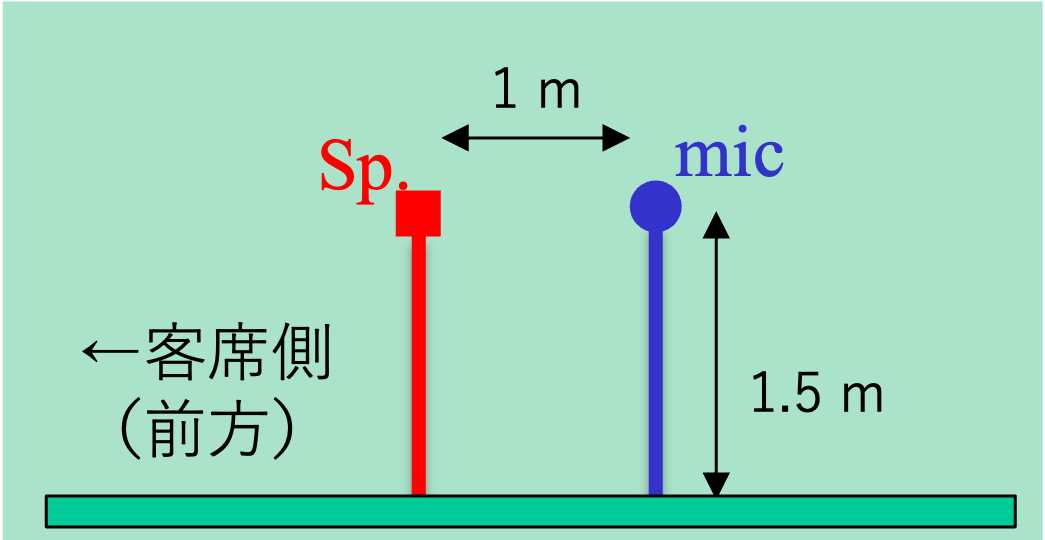
\includegraphics[width=6.5cm,clip]{images/howToMeasureST.png}
  \caption{STのインパルス応答測定条件の概略図}
  \label{fig:STのIR測定条件}
\end{figure}

%=======================================================================
\newpage
\subsection*{アンビソニックマイクを用いた測定システム}
本研究における受音系のマイクとして、図\ref{fig:アンビソニックマイク}に示す商用のアンビソニックマイク(Ambeo VR Mic, Sennheiser)を用いた。アンビソニックマイクは4つのカージオイド特性のマイクを正四面体の頂点方向に配置したものであり、測定後の簡単な信号処理により、全指向性マイクで測定した信号および任意の方向にカージオイド特性のマイクを向けて測定した信号と等価な信号を得ることができる\cite{西村竜一2014}。本研究で用いたアンビソニックマイクの方向に関する定義を図\ref{fig:方向の定義}に示す。

\begin{figure}[H]
  \begin{minipage}[b]{.33\textwidth}
      \centering
      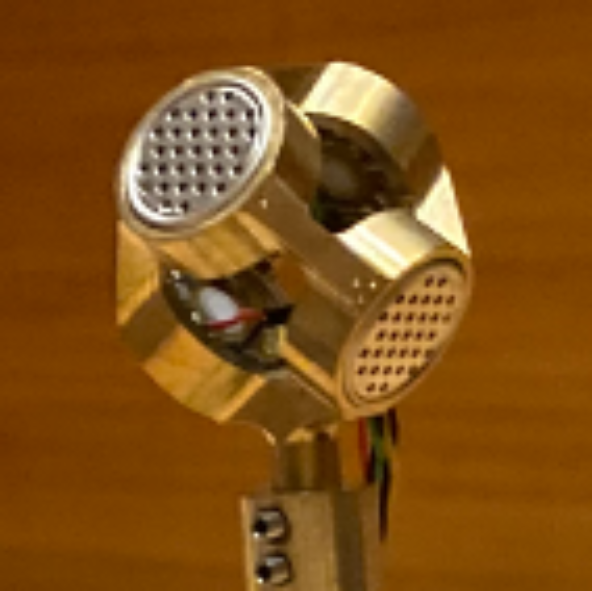
\includegraphics[width=.8\linewidth]{images/ambisonicMic.png}
      \caption{アンビソニックマイク}
      \label{fig:アンビソニックマイク}
  \end{minipage}%
  \begin{minipage}[b]{.66\textwidth}
      \centering
      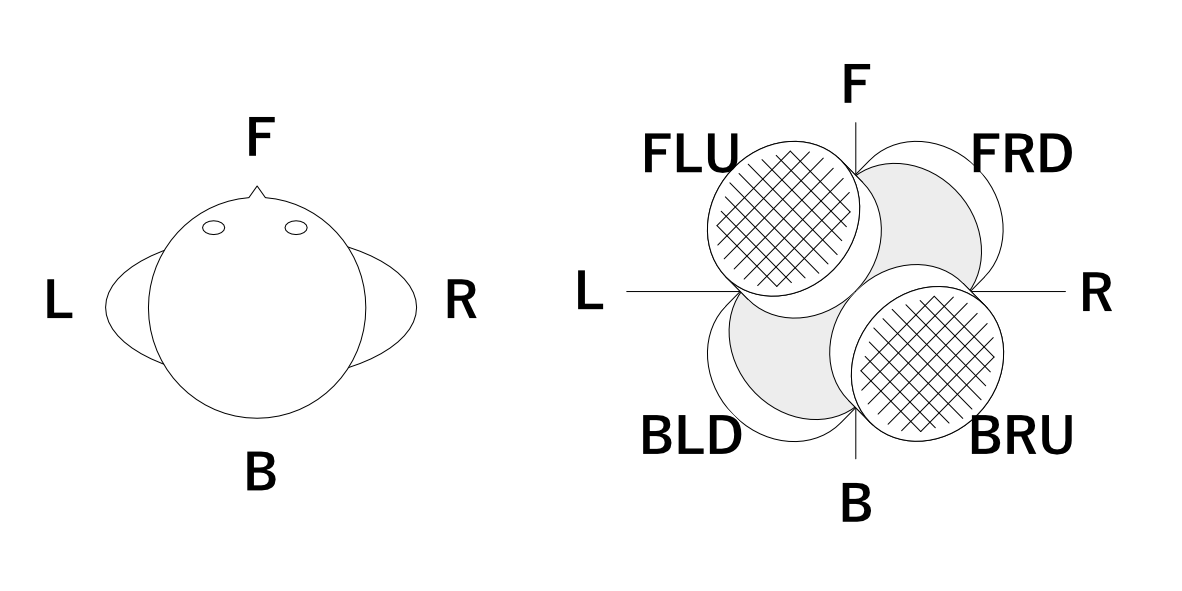
\includegraphics[width=.8\linewidth]{images/ambisonicMicDirectionDef.png}
      \caption{本研究における方向の定義}
      \label{fig:方向の定義}
  \end{minipage}
\end{figure}

方向別インパルス応答を得る手順は次の通りである。まず、Aフォーマットと呼ばれる正四面体の頂点方向の信号から式(\ref{ambisonicAtoB})により全指向性の信号と互いに直交する3つの双指向性の信号からなるBフォーマットと呼ばれる信号を得る。続いて、式(\ref{ambisonicBtoDir})によりBフォーマットの信号から直交6方向の方向別インパルス応答を計算する。

ここで、$p_(t)$は全指向性マイクで測定したインパルス応答と等価な信号、$p_{\mathrm{FB}}(t)$、$p_{\mathrm{LR}}(t)$、$p_{\mathrm{UD}}(t)$は前後、左右、上下の双指向性マイクで収録したインパルス応答と等価な信号を表し、$p_{\mathrm{FLU}}$、$p_{\mathrm{FRD}}$、$p_{\mathrm{BLD}}$、$p_{\mathrm{BRU}}$はアンビソニックマイクのうち前方左上方(Front Left Up)、前方右下方(Front Right Down)、後方左下方(Back Left Down)、後方右上方(Back Right Up)の信号を表す。
\begin{equation}
  \label{ambisonicAtoB}
  \begin{alignedat}{4}
    p_(t) &= \frac{1}{2} (p_{\mathrm{FLU}} + p_{\mathrm{FRD}} + p_{\mathrm{BLD}} + p_{\mathrm{BRU}})
    \\
    p_{\mathrm{FB}}(t) &= \frac{\sqrt{3}}{2} (p_{\mathrm{FLU}} + p_{\mathrm{FRD}} - p_{\mathrm{BLD}} - p_{\mathrm{BRU}})
    \\
    p_{\mathrm{LR}}(t) &= \frac{\sqrt{3}}{2} (p_{\mathrm{FLU}} - p_{\mathrm{FRD}} + p_{\mathrm{BLD}} - p_{\mathrm{BRU}})
    \\
    p_{\mathrm{UD}}(t) &= \frac{\sqrt{3}}{2} (p_{\mathrm{FLU}} - p_{\mathrm{FRD}} - p_{\mathrm{BLD}} + p_{\mathrm{BRU}})
    \\
  \end{alignedat}
\end{equation}
\begin{equation}
  \label{ambisonicBtoDir}
  \begin{alignedat}{6}
    p_{\mathrm{F}}(t) &= \frac{1}{2} (p(t) + p_{\mathrm{FB}}(t))
    \\
    p_{\mathrm{B}}(t) &= \frac{1}{2} (p(t) - p_{\mathrm{FB}}(t))
    \\
    p_{\mathrm{L}}(t) &= \frac{1}{2} (p(t) + p_{\mathrm{LR}}(t))
    \\
    p_{\mathrm{R}}(t) &= \frac{1}{2} (p(t) - p_{\mathrm{LR}}(t))
    \\
    p_{\mathrm{U}}(t) &= \frac{1}{2} (p(t) + p_{\mathrm{UD}}(t))
    \\
    p_{\mathrm{D}}(t) &= \frac{1}{2} (p(t) - p_{\mathrm{UD}}(t)) \\
  \end{alignedat}
\end{equation}

%=======================================================================
\section{方向別STの実測}

\subsection*{測定方法および測定結果}
前節で提案した方向別STについて、室形状・空間規模の異なる複数のホールの多数点で方向別
実測を行い、現実のホールステージにおける反射音到来方向特性を把握する。音源には図\ref{fig:対向スピーカー}に示す無指向性の対向スピーカー、マイクロホンには図\ref{fig:アンビソニックマイク}に示す商用の1次アンビソニックマイク(Ambeo VR Mic, Sennheiser)を使用した。

音響測定を実施した各ホールの諸元を\ref{table:全ホールの諸元}に示す。ホールAからFは舞台を反射板形式とした多目的ホール、ホールGはアリーナ型のコンサートホールである。なお、ホールBは天井反射板が無い舞台となっている。また、測定を実施した各ホールの外観を\ref{fig:全ホールの写真}に示す。測定点は各ホールの舞台の上手側半面に$\SI{2}{\m}$間隔のグリッド上に配置した。\ref{fig:各ホールの測定位置}に各ホールにおける測定点の音源位置を示す。全ての測定点において音源を客席側、マイクを舞台奥側に配置している。

各ホールのすべての測定点における測定結果を図\ref{fig:ホールA 方向別ST}から図\ref{fig:ホールG 方向別ST}に示す。測定位置によって$\SI{10}{\ms}$から$\SI{20}{\ms}$にも反射音のエネルギーが到来し、これも踏まえた考察を行うため、前節で提案した$\mathrm{ST_{Early,dir}}$および$\mathrm{ST_{Late,dir}}$に加え、$\SI{10}{\ms}$から$\SI{100}{\ms}$の時間窓で反射音を評価した結果についても合わせて示した。
\\

\begin{figure}[H]
  \centering
  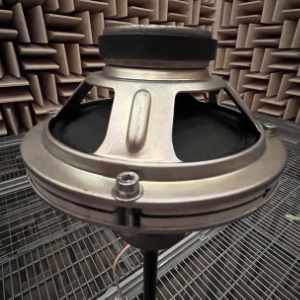
\includegraphics[width=.3\linewidth]{images/measuredHalls/opposedSpeaker.jpg}
  \caption{対向スピーカー}
  \label{fig:対向スピーカー}
\end{figure}

\begin{table}[H]
  \centering
  \caption{測定を実施したホールの諸元}
  \label{table:全ホールの諸元}
  \begin{tabular}{cccccccc} \hline \hline
    ホール &
    \begin{tabular}{c}
      座席数\\
      (席)
    \end{tabular}& 
    \begin{tabular}{c}
      $\mathrm{T_{30}}$(s) 500-\\
      1kHz平均
    \end{tabular}&
    \begin{tabular}{c}
      室容積\\
      ($\mathrm{m^{3}}$)
    \end{tabular}&
    \begin{tabular}{c}
      表面積\\
      ($\mathrm{m^{2}}$) 
    \end{tabular}&
    \begin{tabular}{c}
      舞台間口\\
      (m)
    \end{tabular}&
    \begin{tabular}{c}
      舞台奥行\\
      (m)
    \end{tabular}&
    \begin{tabular}{c}
      舞台高さ\\(m)
    \end{tabular} \\ \hline
    A & 421 & 1.3 & 4420 & 2070 & 16.5 & 10.5 & 8 \\
    B & 500 & 1.4 & 5680 & 2740 & 15.5 & 9 & 7.4 \\
    C & 698 & 2.5 & 11150 & 4600 & 12 & 16.2 & 13 \\
    D & 1033 & 1.9 & 11940 & 4380 & 20 & 10 & 10 \\
    E & 1104 & 1.6 & 10225 & 3435 & 19 & 9 & 8 \\
    F & 1514 & 2.3 & 15580 & 5860 & 18.2 & 18.2 & 15 \\
    G & 1884 & 2.2 & 18610 & 6445 & 20.8 & 11.7 & - \\ \hline \hline
  \end{tabular}
\end{table}

%=======================================================================

\newpage
\begin{figure}[H]
  \centering
  \begin{minipage}[b]{.5\textwidth}
    \centering
    \includegraphics[width=.9\linewidth]{images/measuredHalls/w90h60/picture_a.jpg}
    \caption*{ホールA}
  \end{minipage}%
  \begin{minipage}[b]{.5\textwidth}
    \centering
    \includegraphics[width=.9\linewidth]{images/measuredHalls/w90h60/picture_b.jpg}
    \caption*{ホールB}
  \end{minipage}

  \begin{minipage}[b]{.5\textwidth}
    \centering
    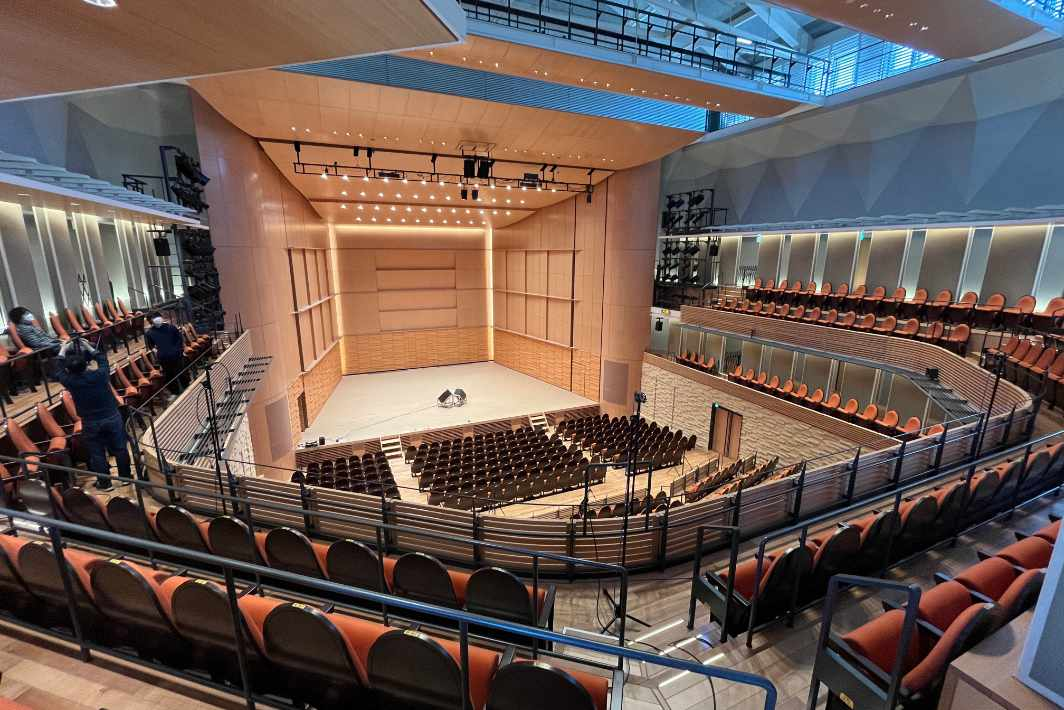
\includegraphics[width=.9\linewidth]{images/measuredHalls/w90h60/picture_c.jpg}
    \caption*{ホールC}
  \end{minipage}%
  \begin{minipage}[b]{.5\textwidth}
    \centering
    \includegraphics[width=.9\linewidth]{images/measuredHalls/w90h60/picture_d.jpg}
    \caption*{ホールD}
  \end{minipage}

  \begin{minipage}[b]{.5\textwidth}
    \centering
    \includegraphics[width=.9\linewidth]{images/measuredHalls/w90h60/picture_e.jpg}
    \caption*{ホールE}
  \end{minipage}%
  \begin{minipage}[b]{.5\textwidth}
    \centering
    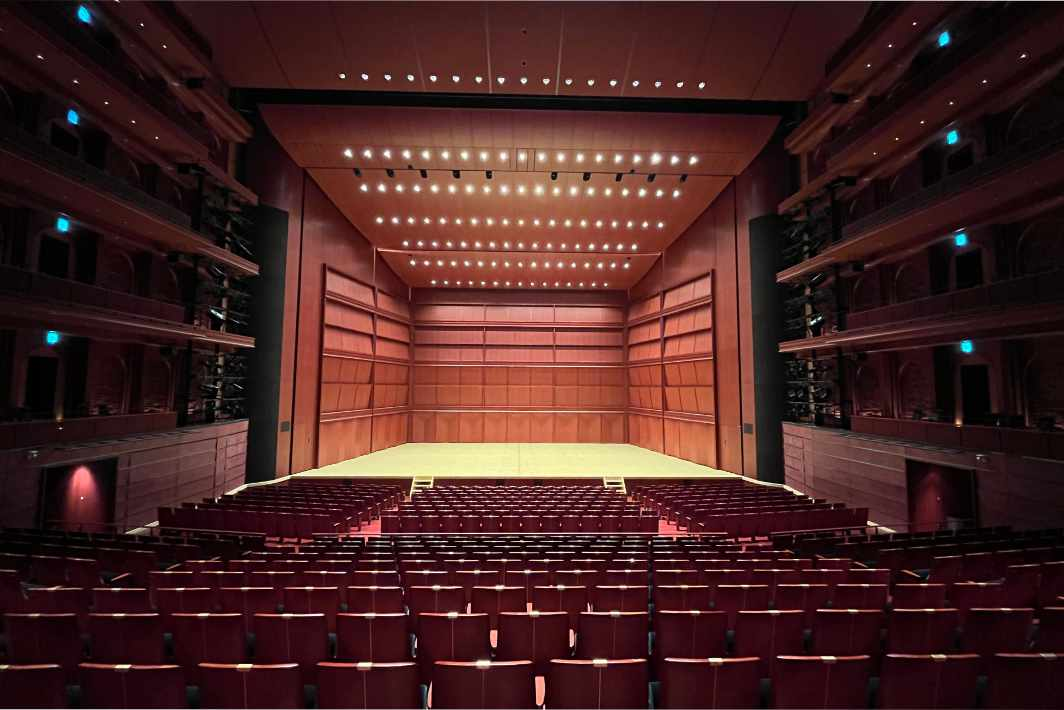
\includegraphics[width=.9\linewidth]{images/measuredHalls/w90h60/picture_f.jpg}
    \caption*{ホールF}
  \end{minipage}

  \begin{minipage}[b]{1\textwidth}
    \centering
    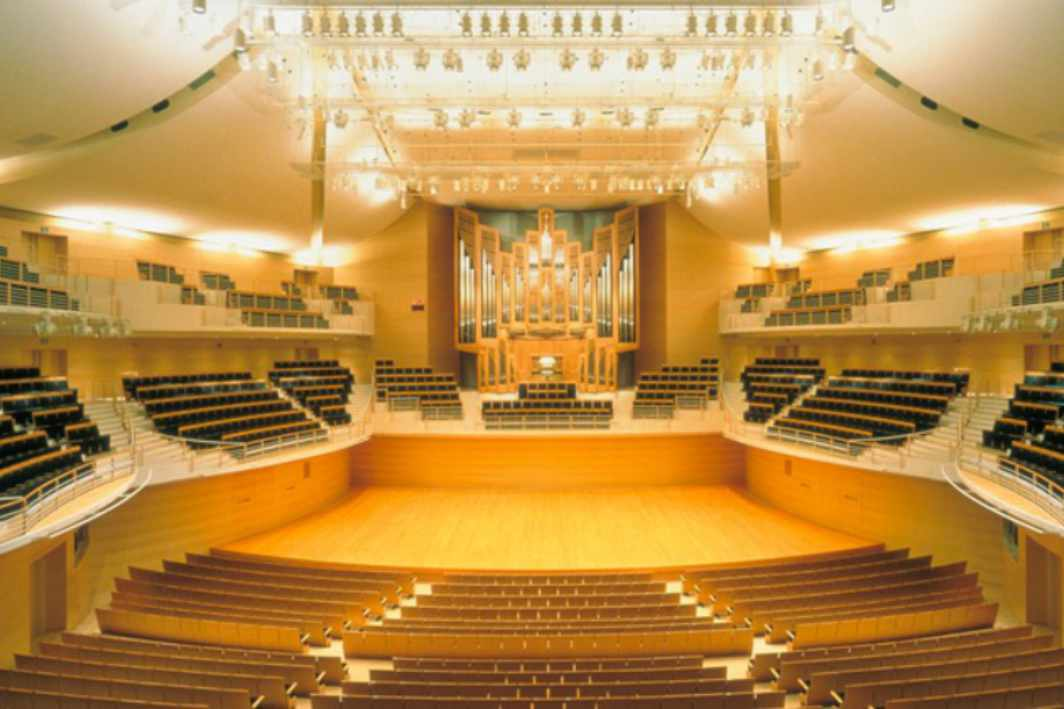
\includegraphics[width=.45\linewidth]{images/measuredHalls/w90h60/picture_g.jpg}
    \caption*{ホールG}
  \end{minipage}

  \caption{測定を実施したホールの外観}
  \label{fig:全ホールの写真}
\end{figure}

%=======================================================================

\newpage
\begin{figure}[H]
  \centering
  \begin{minipage}[b]{.5\textwidth}
    \centering
    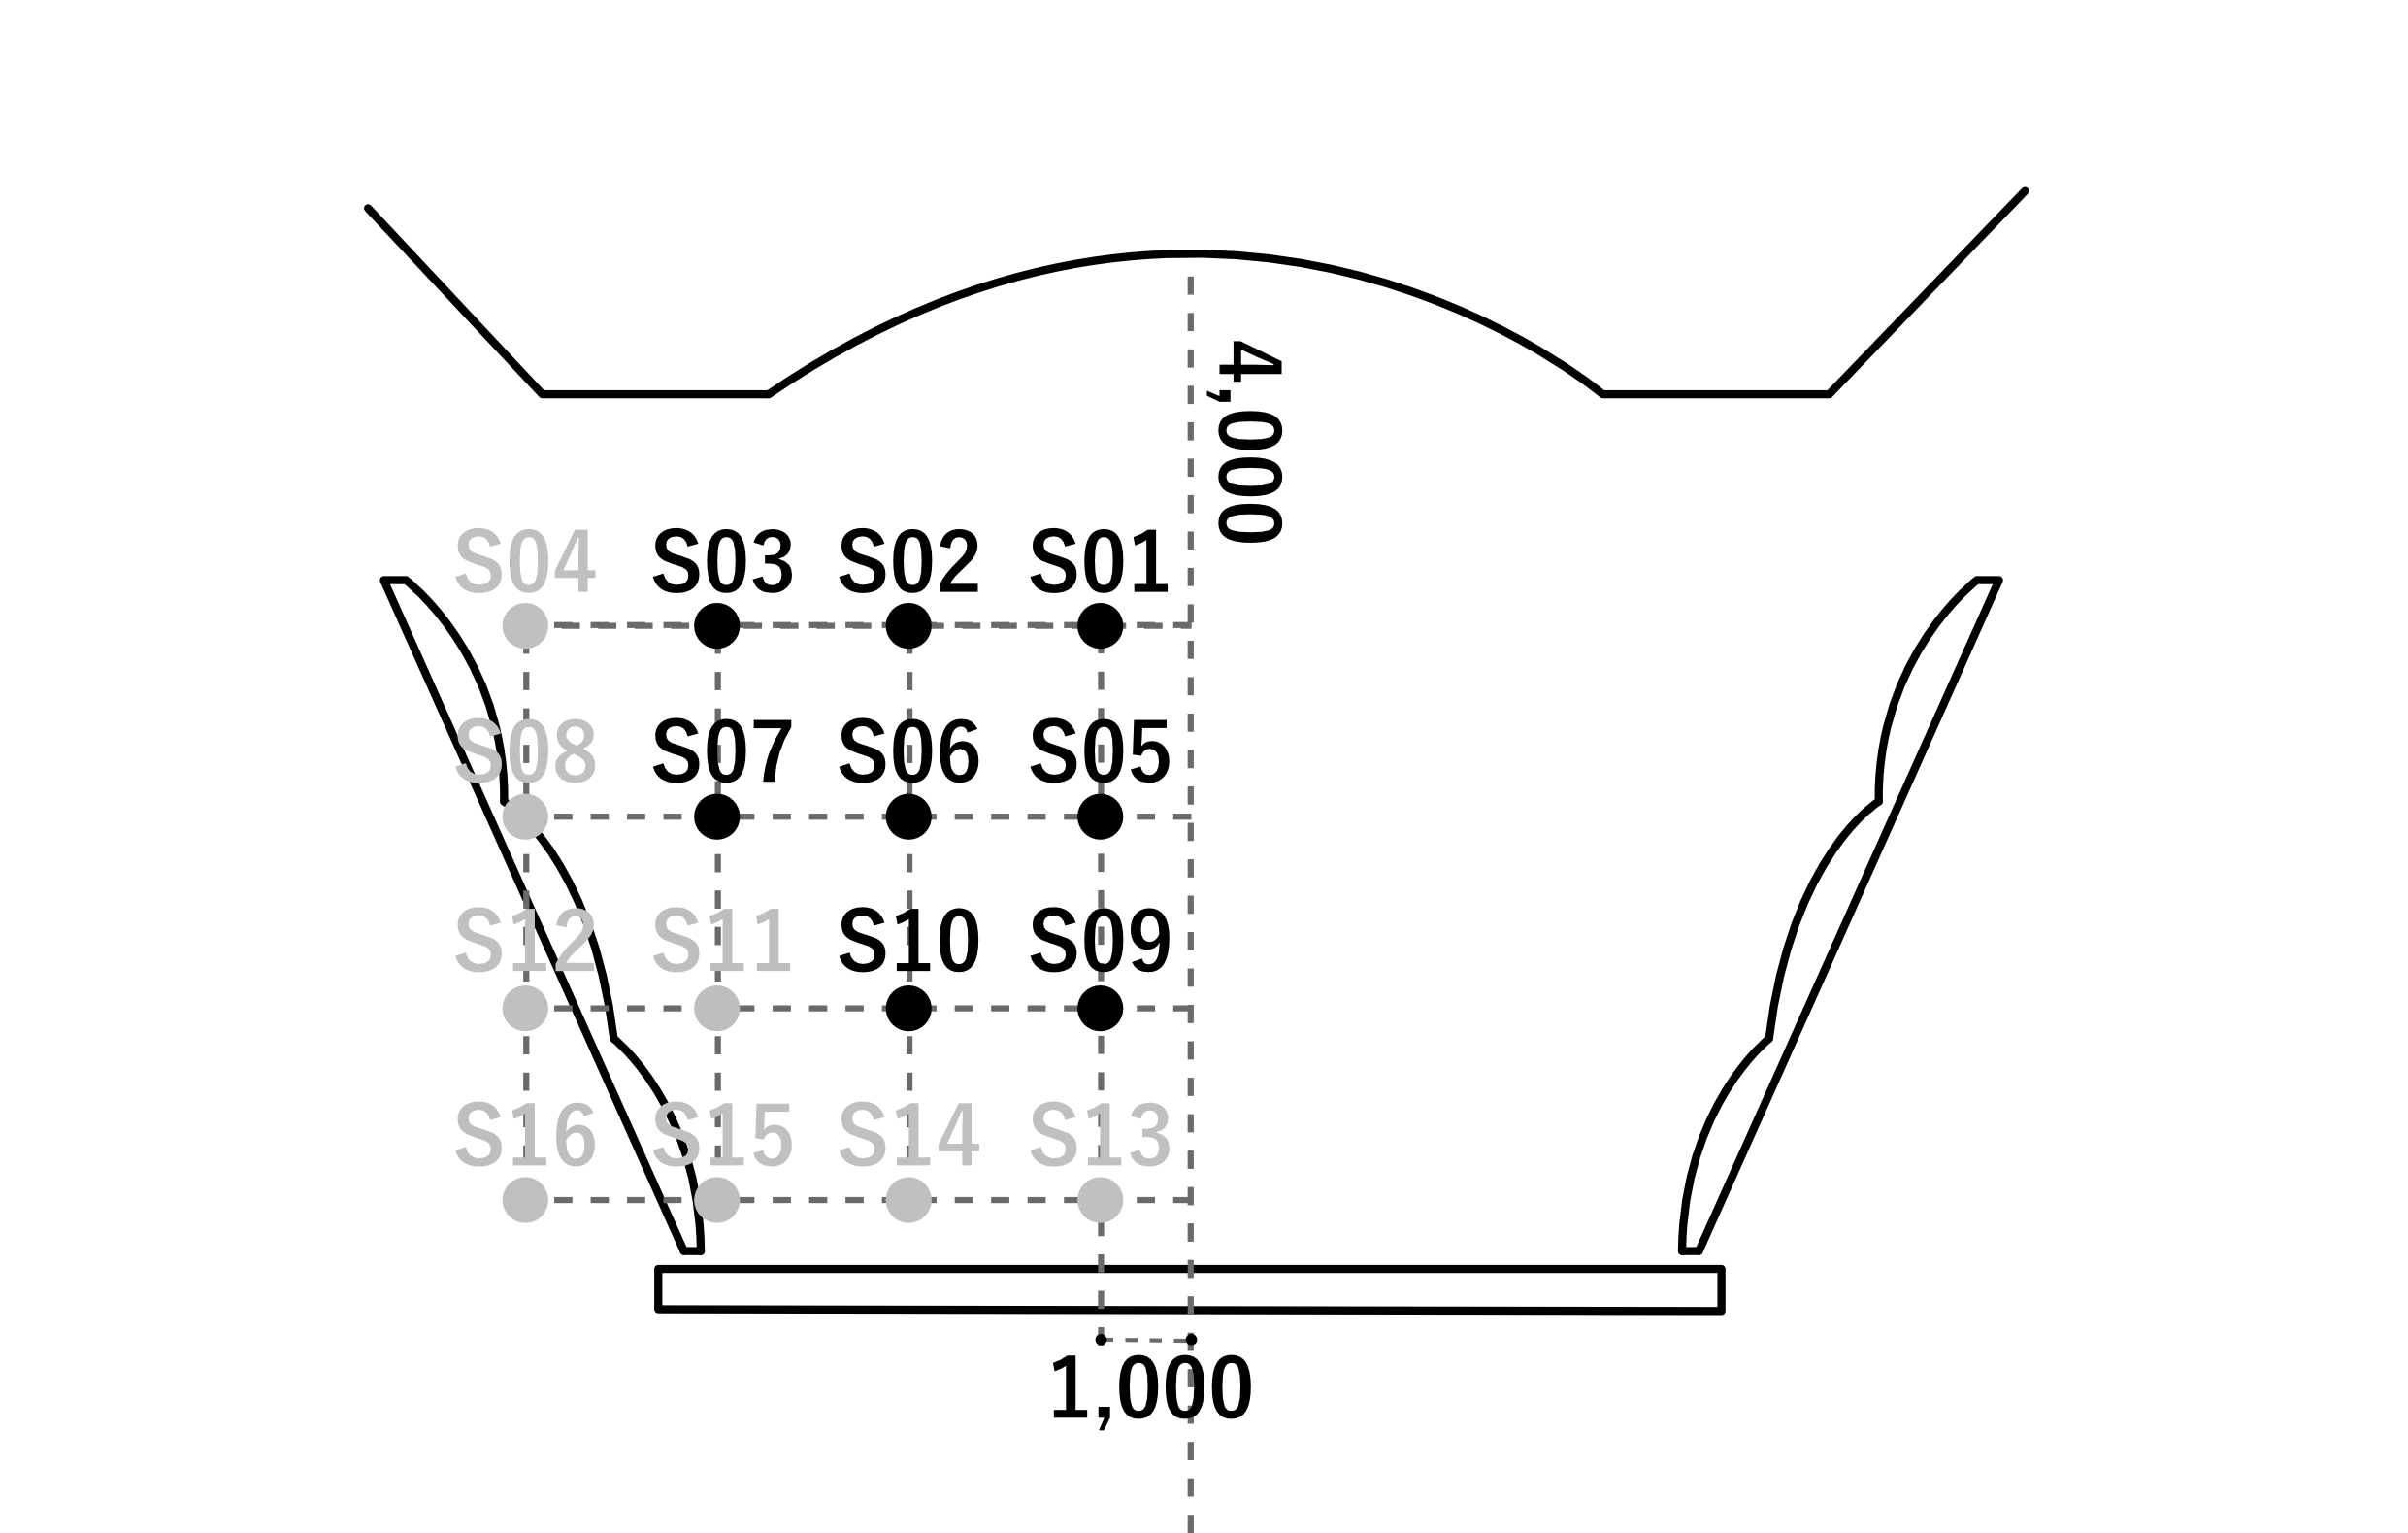
\includegraphics[width=.9\linewidth]{images/measuredHalls/flatud_hall_a.png}
    \caption*{ホールA}
  \end{minipage}%
  \begin{minipage}[b]{.5\textwidth}
    \centering
    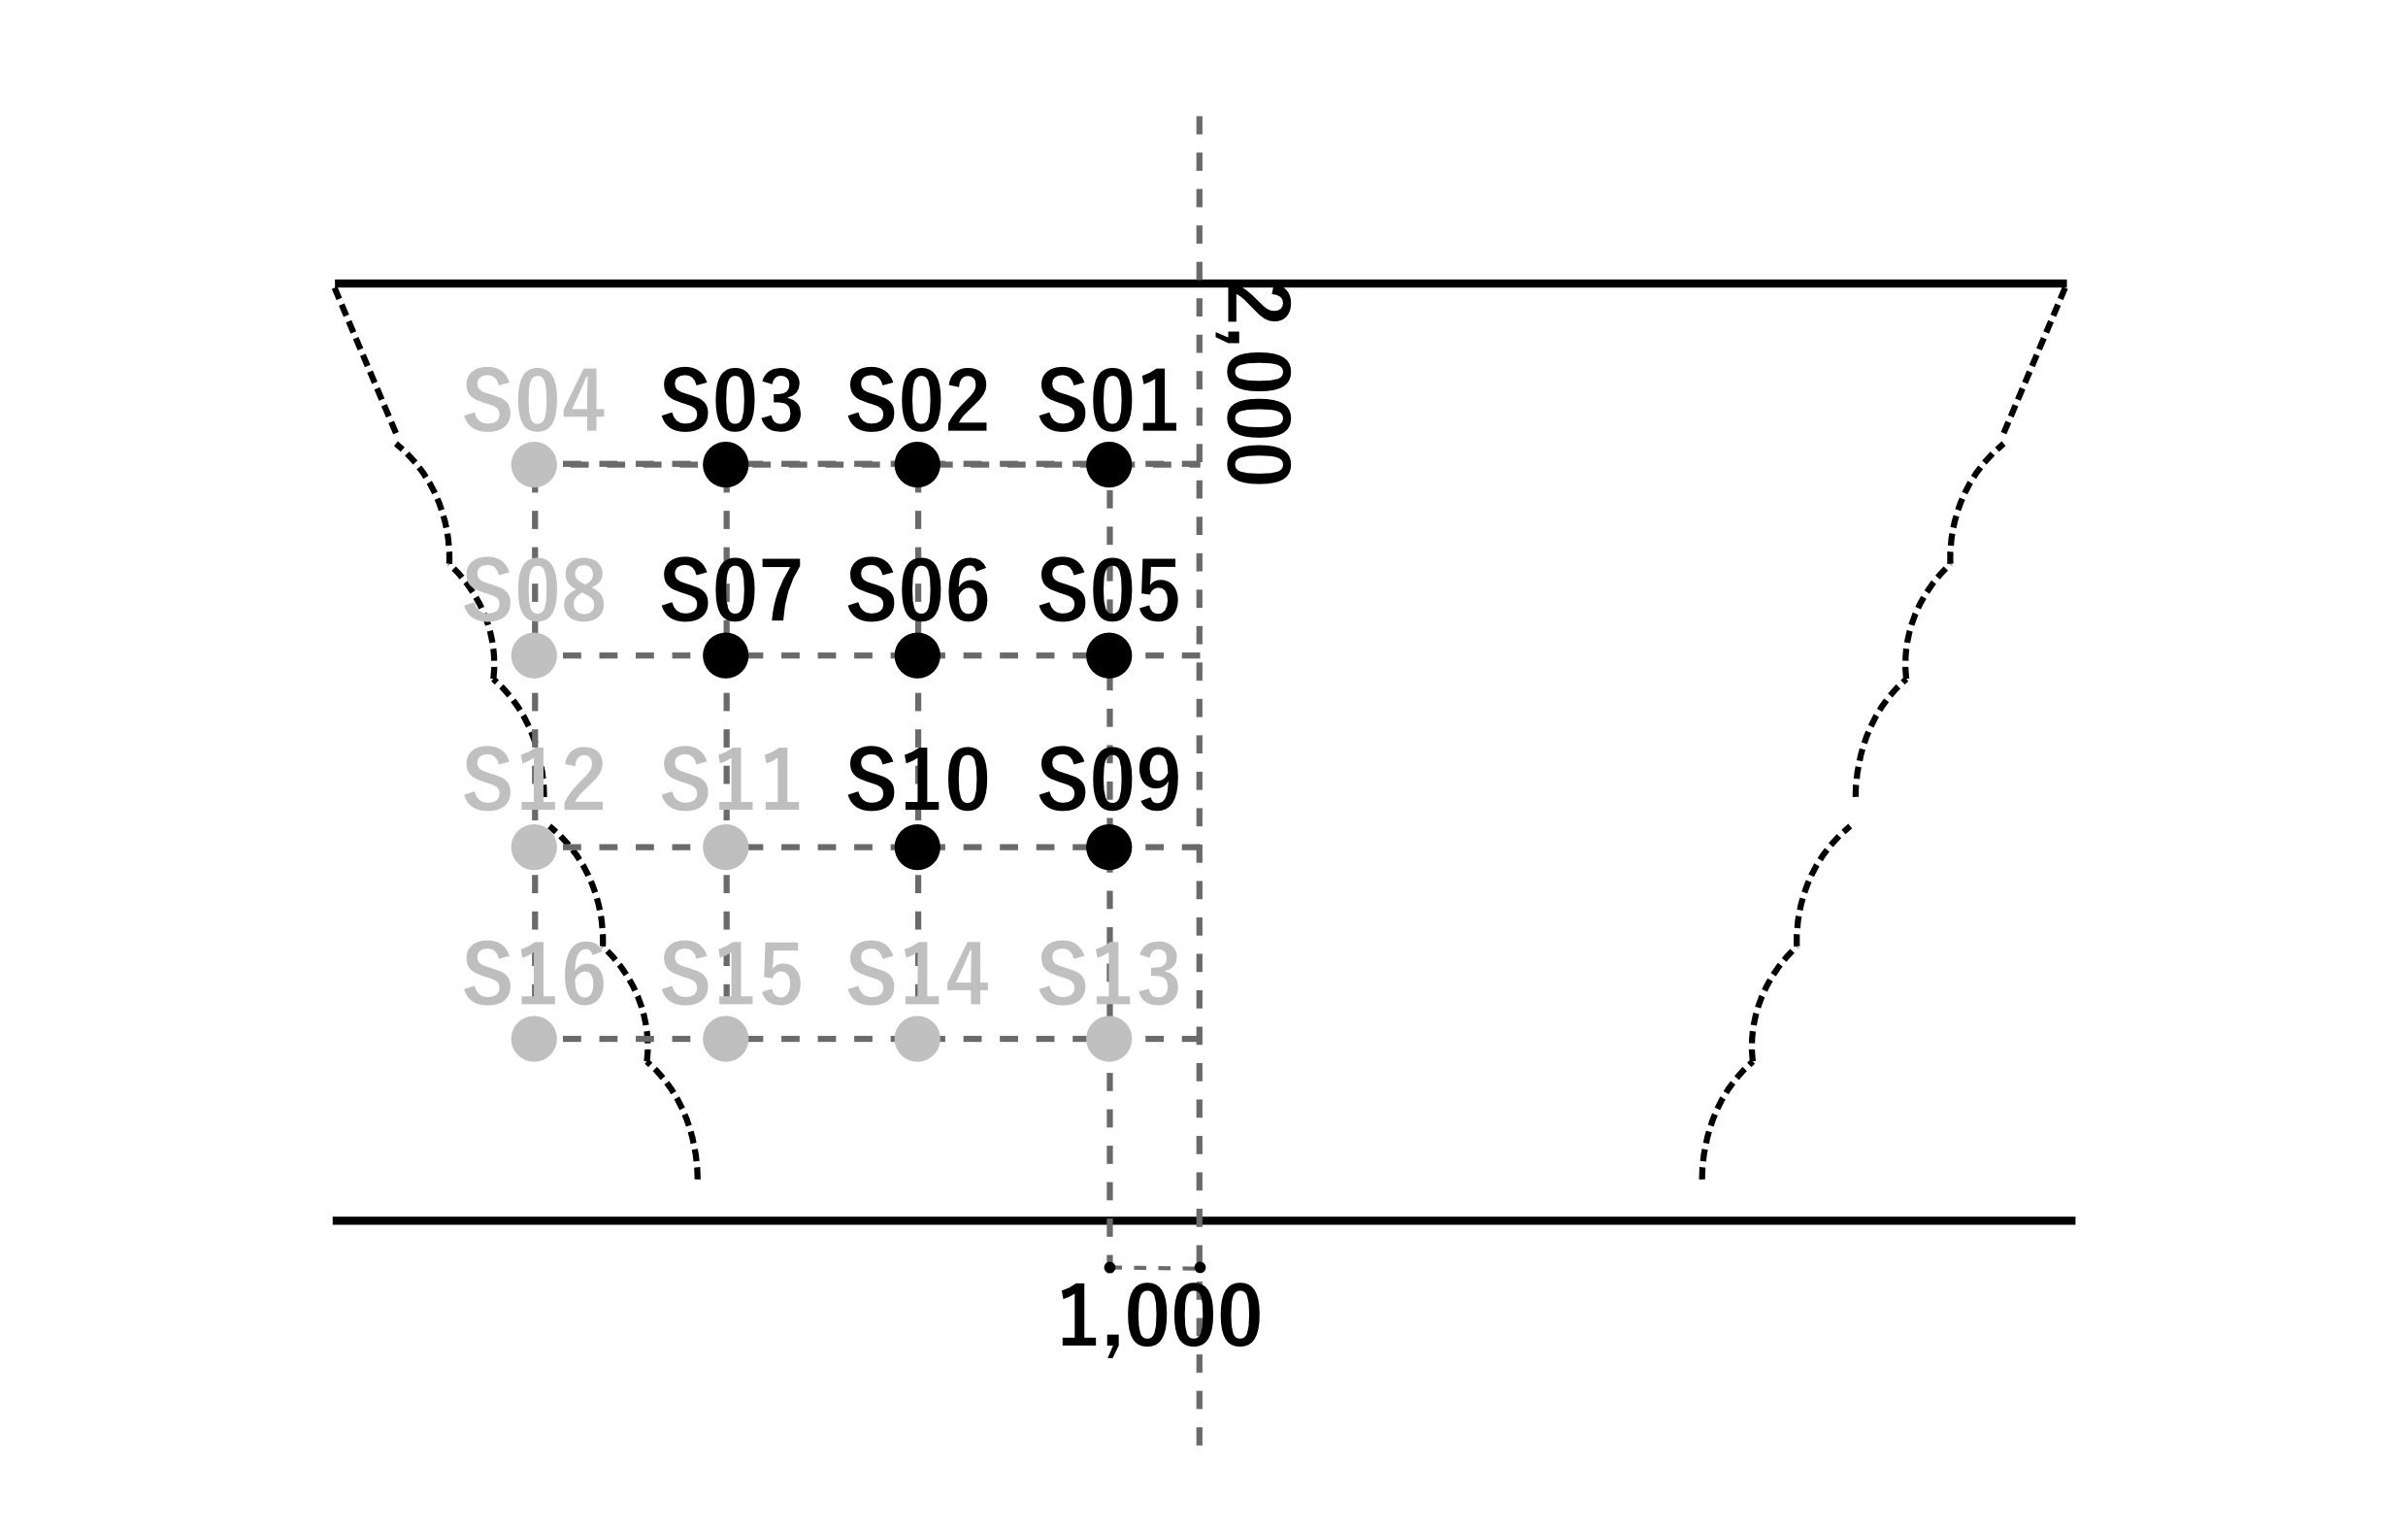
\includegraphics[width=.9\linewidth]{images/measuredHalls/flatud_hall_b.png}
    \caption*{ホールB}
  \end{minipage}

  \begin{minipage}[b]{.5\textwidth}
    \centering
    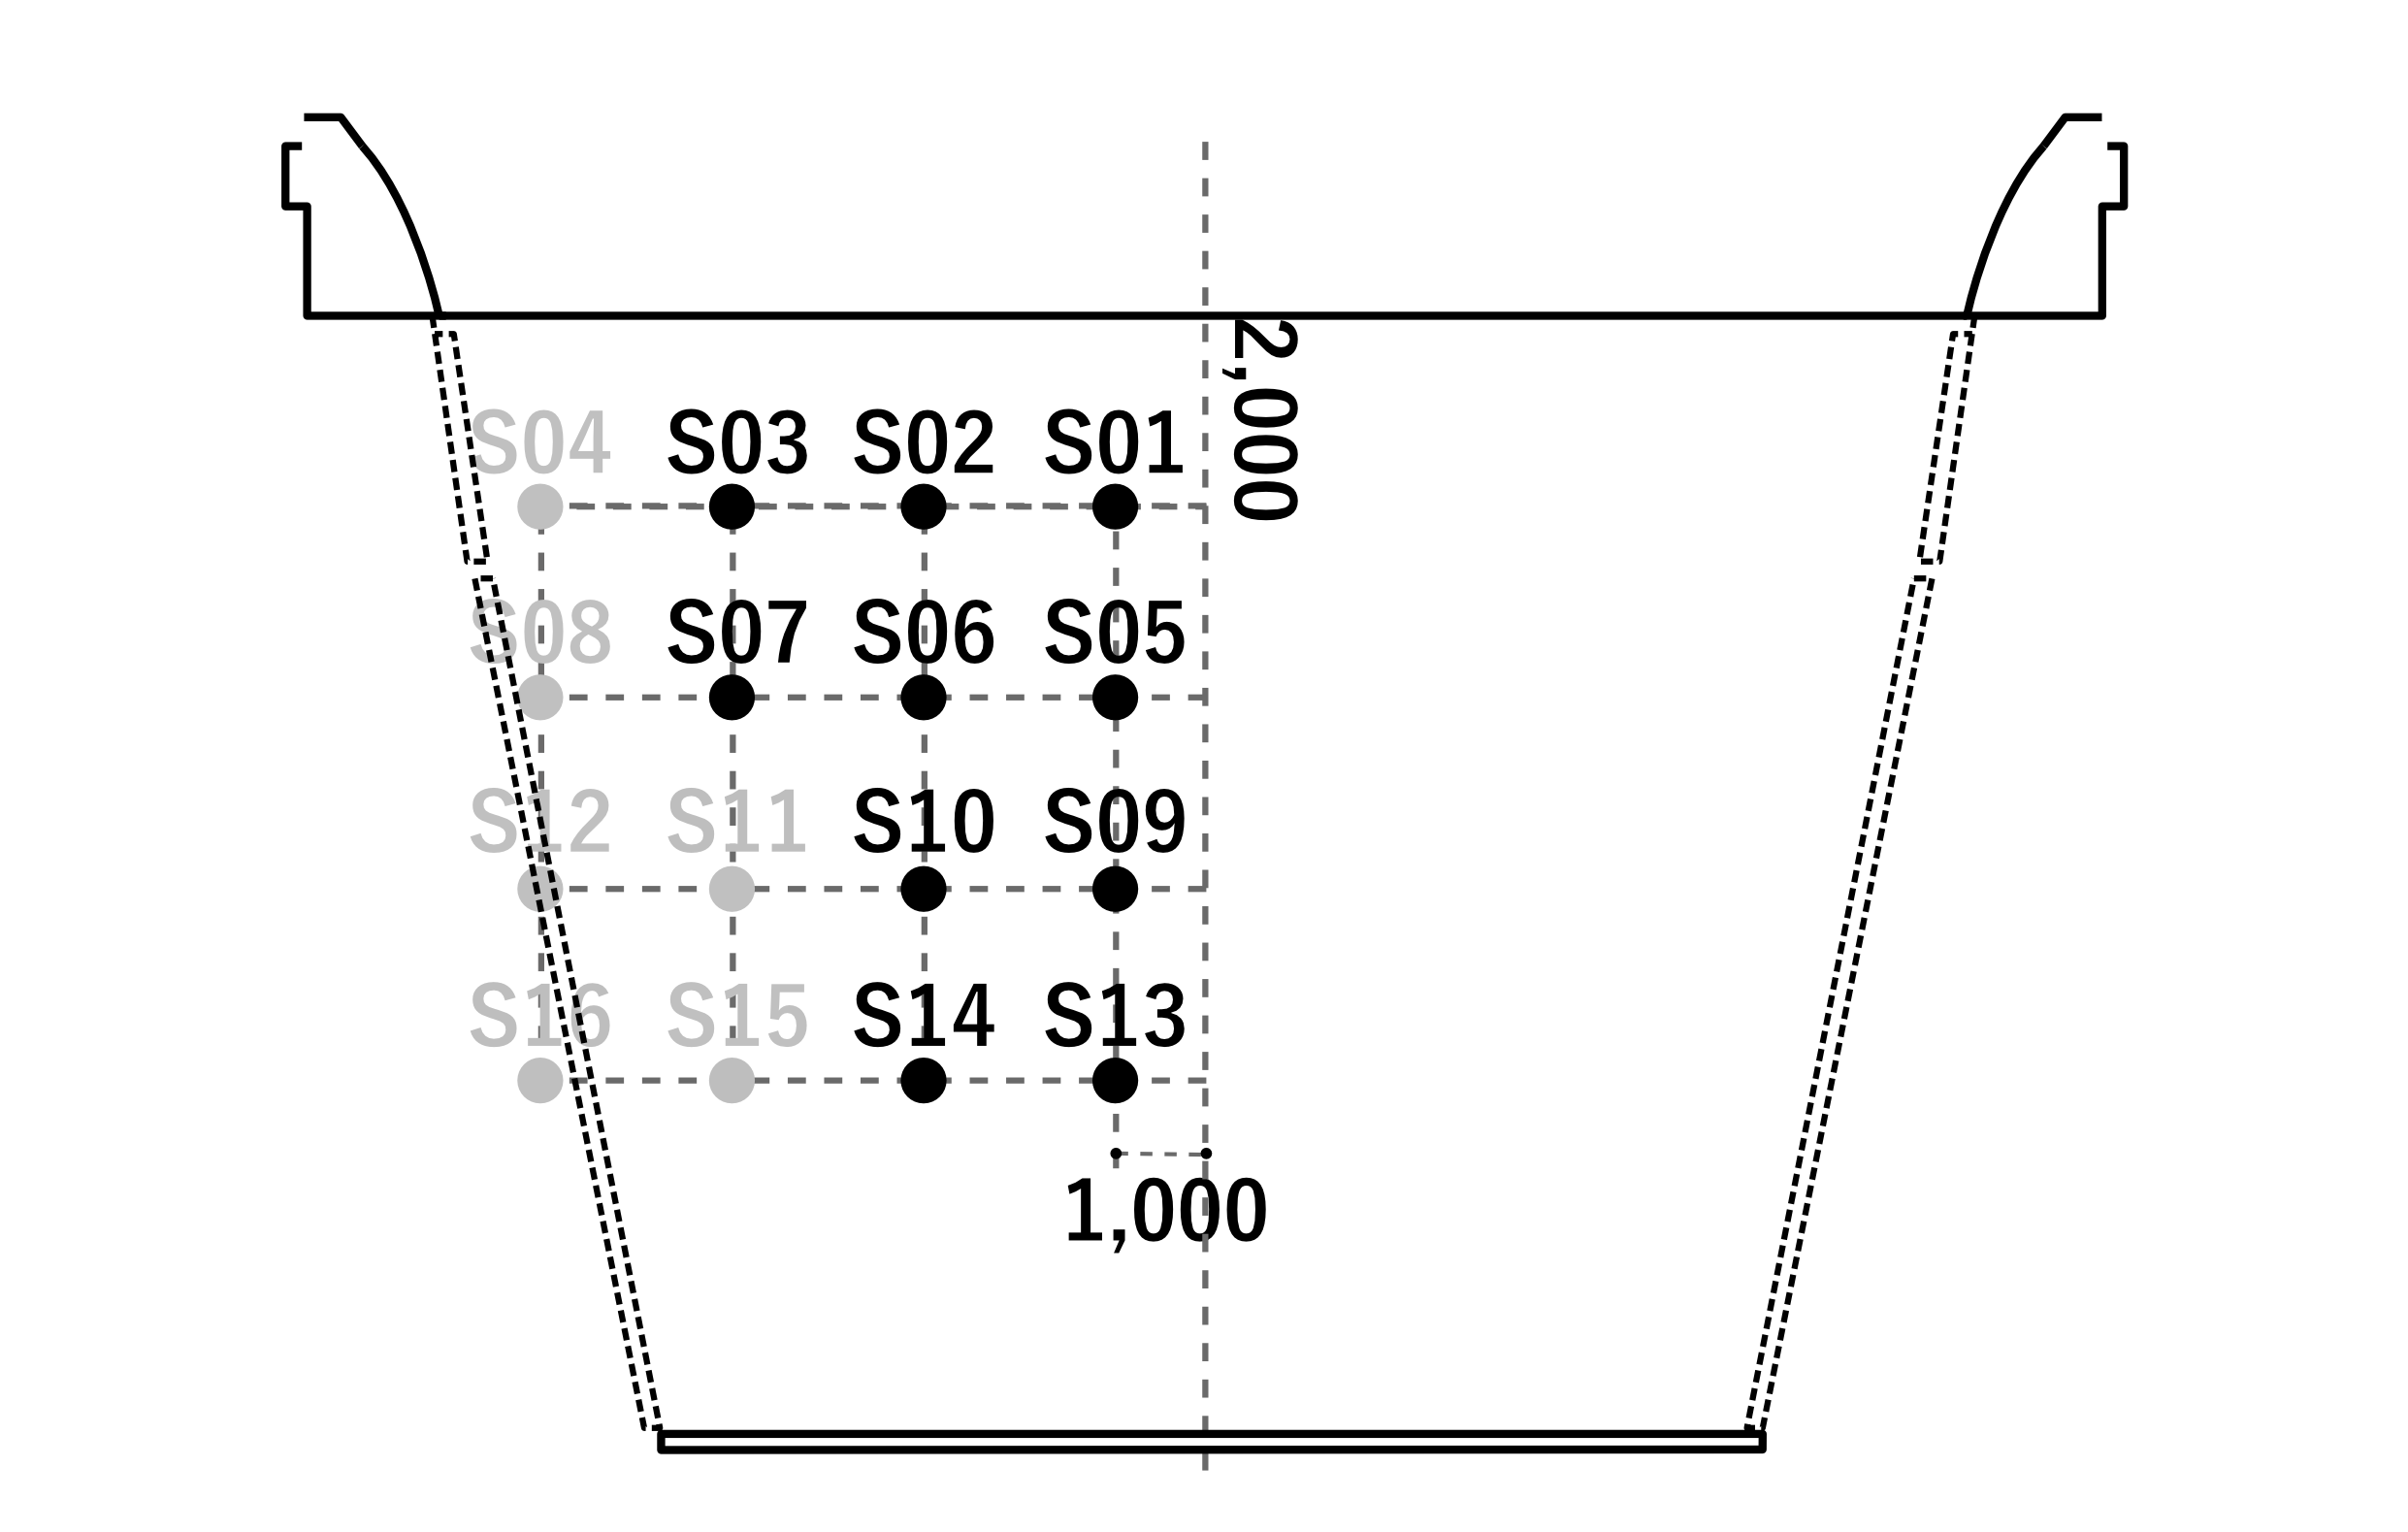
\includegraphics[width=.9\linewidth]{images/measuredHalls/flatud_hall_c.png}
    \caption*{ホールC}
  \end{minipage}%
  \begin{minipage}[b]{.5\textwidth}
    \centering
    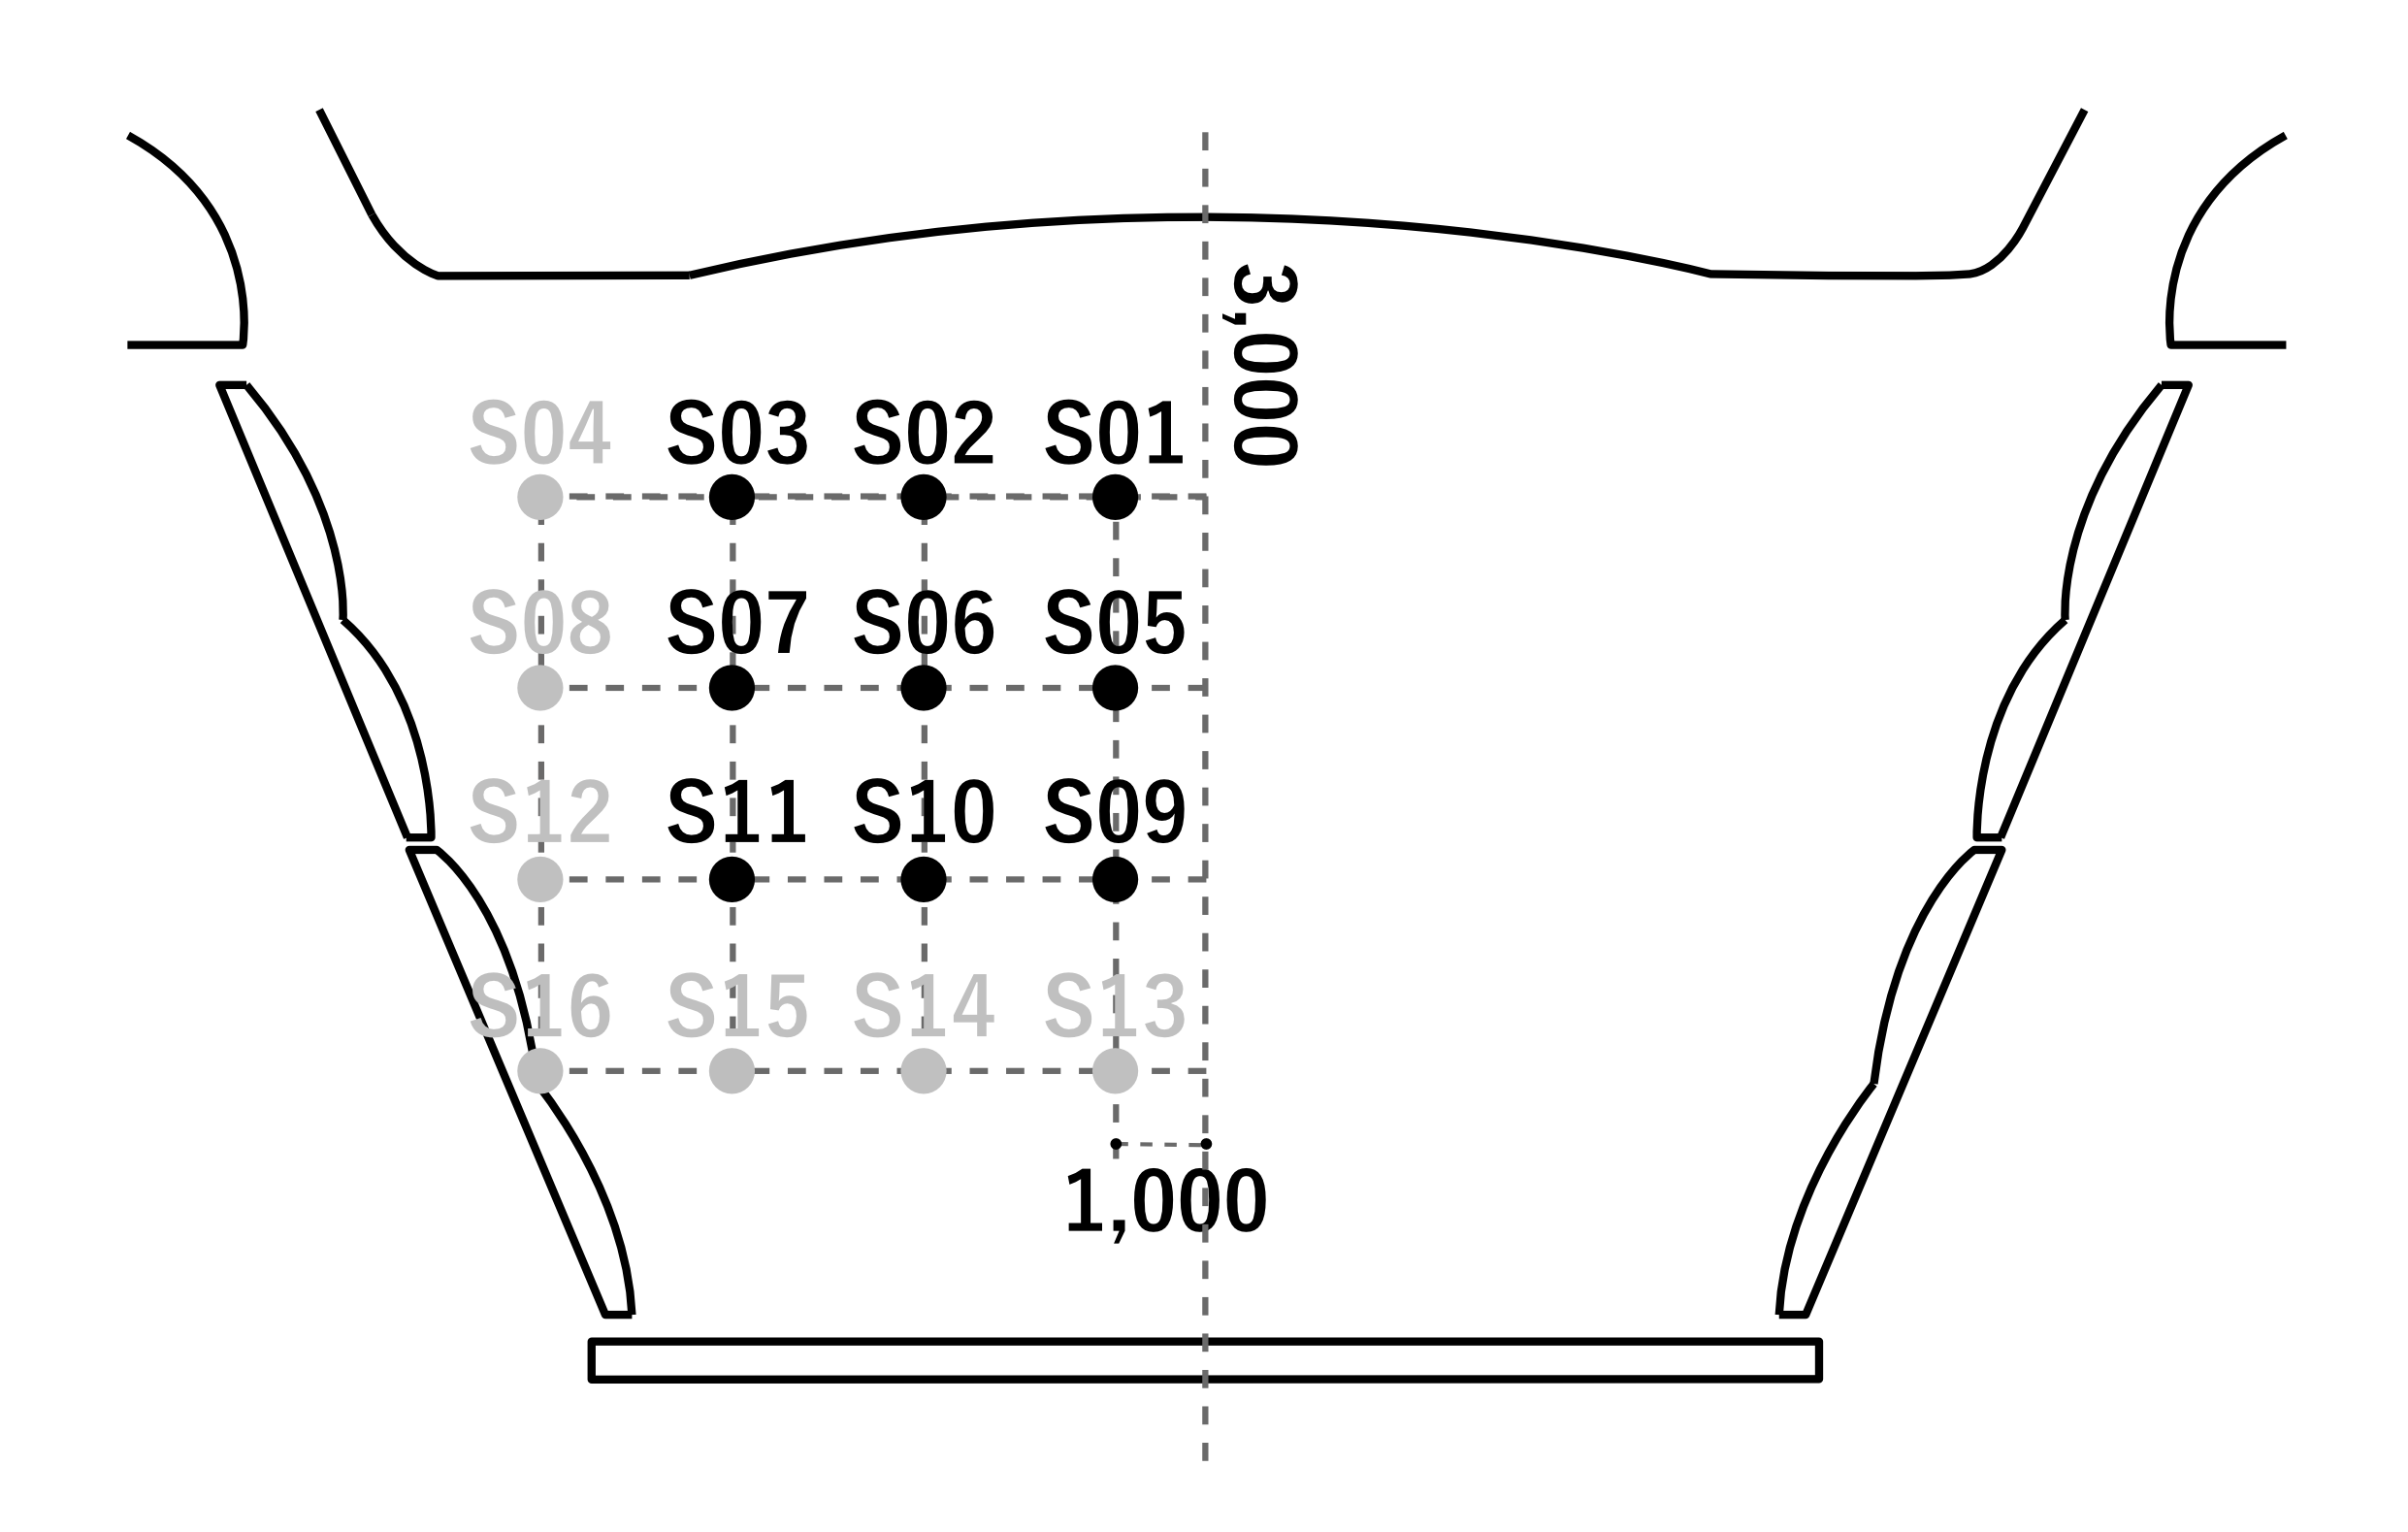
\includegraphics[width=.9\linewidth]{images/measuredHalls/flatud_hall_d.png}
    \caption*{ホールD}
  \end{minipage}

  \begin{minipage}[b]{.5\textwidth}
    \centering
    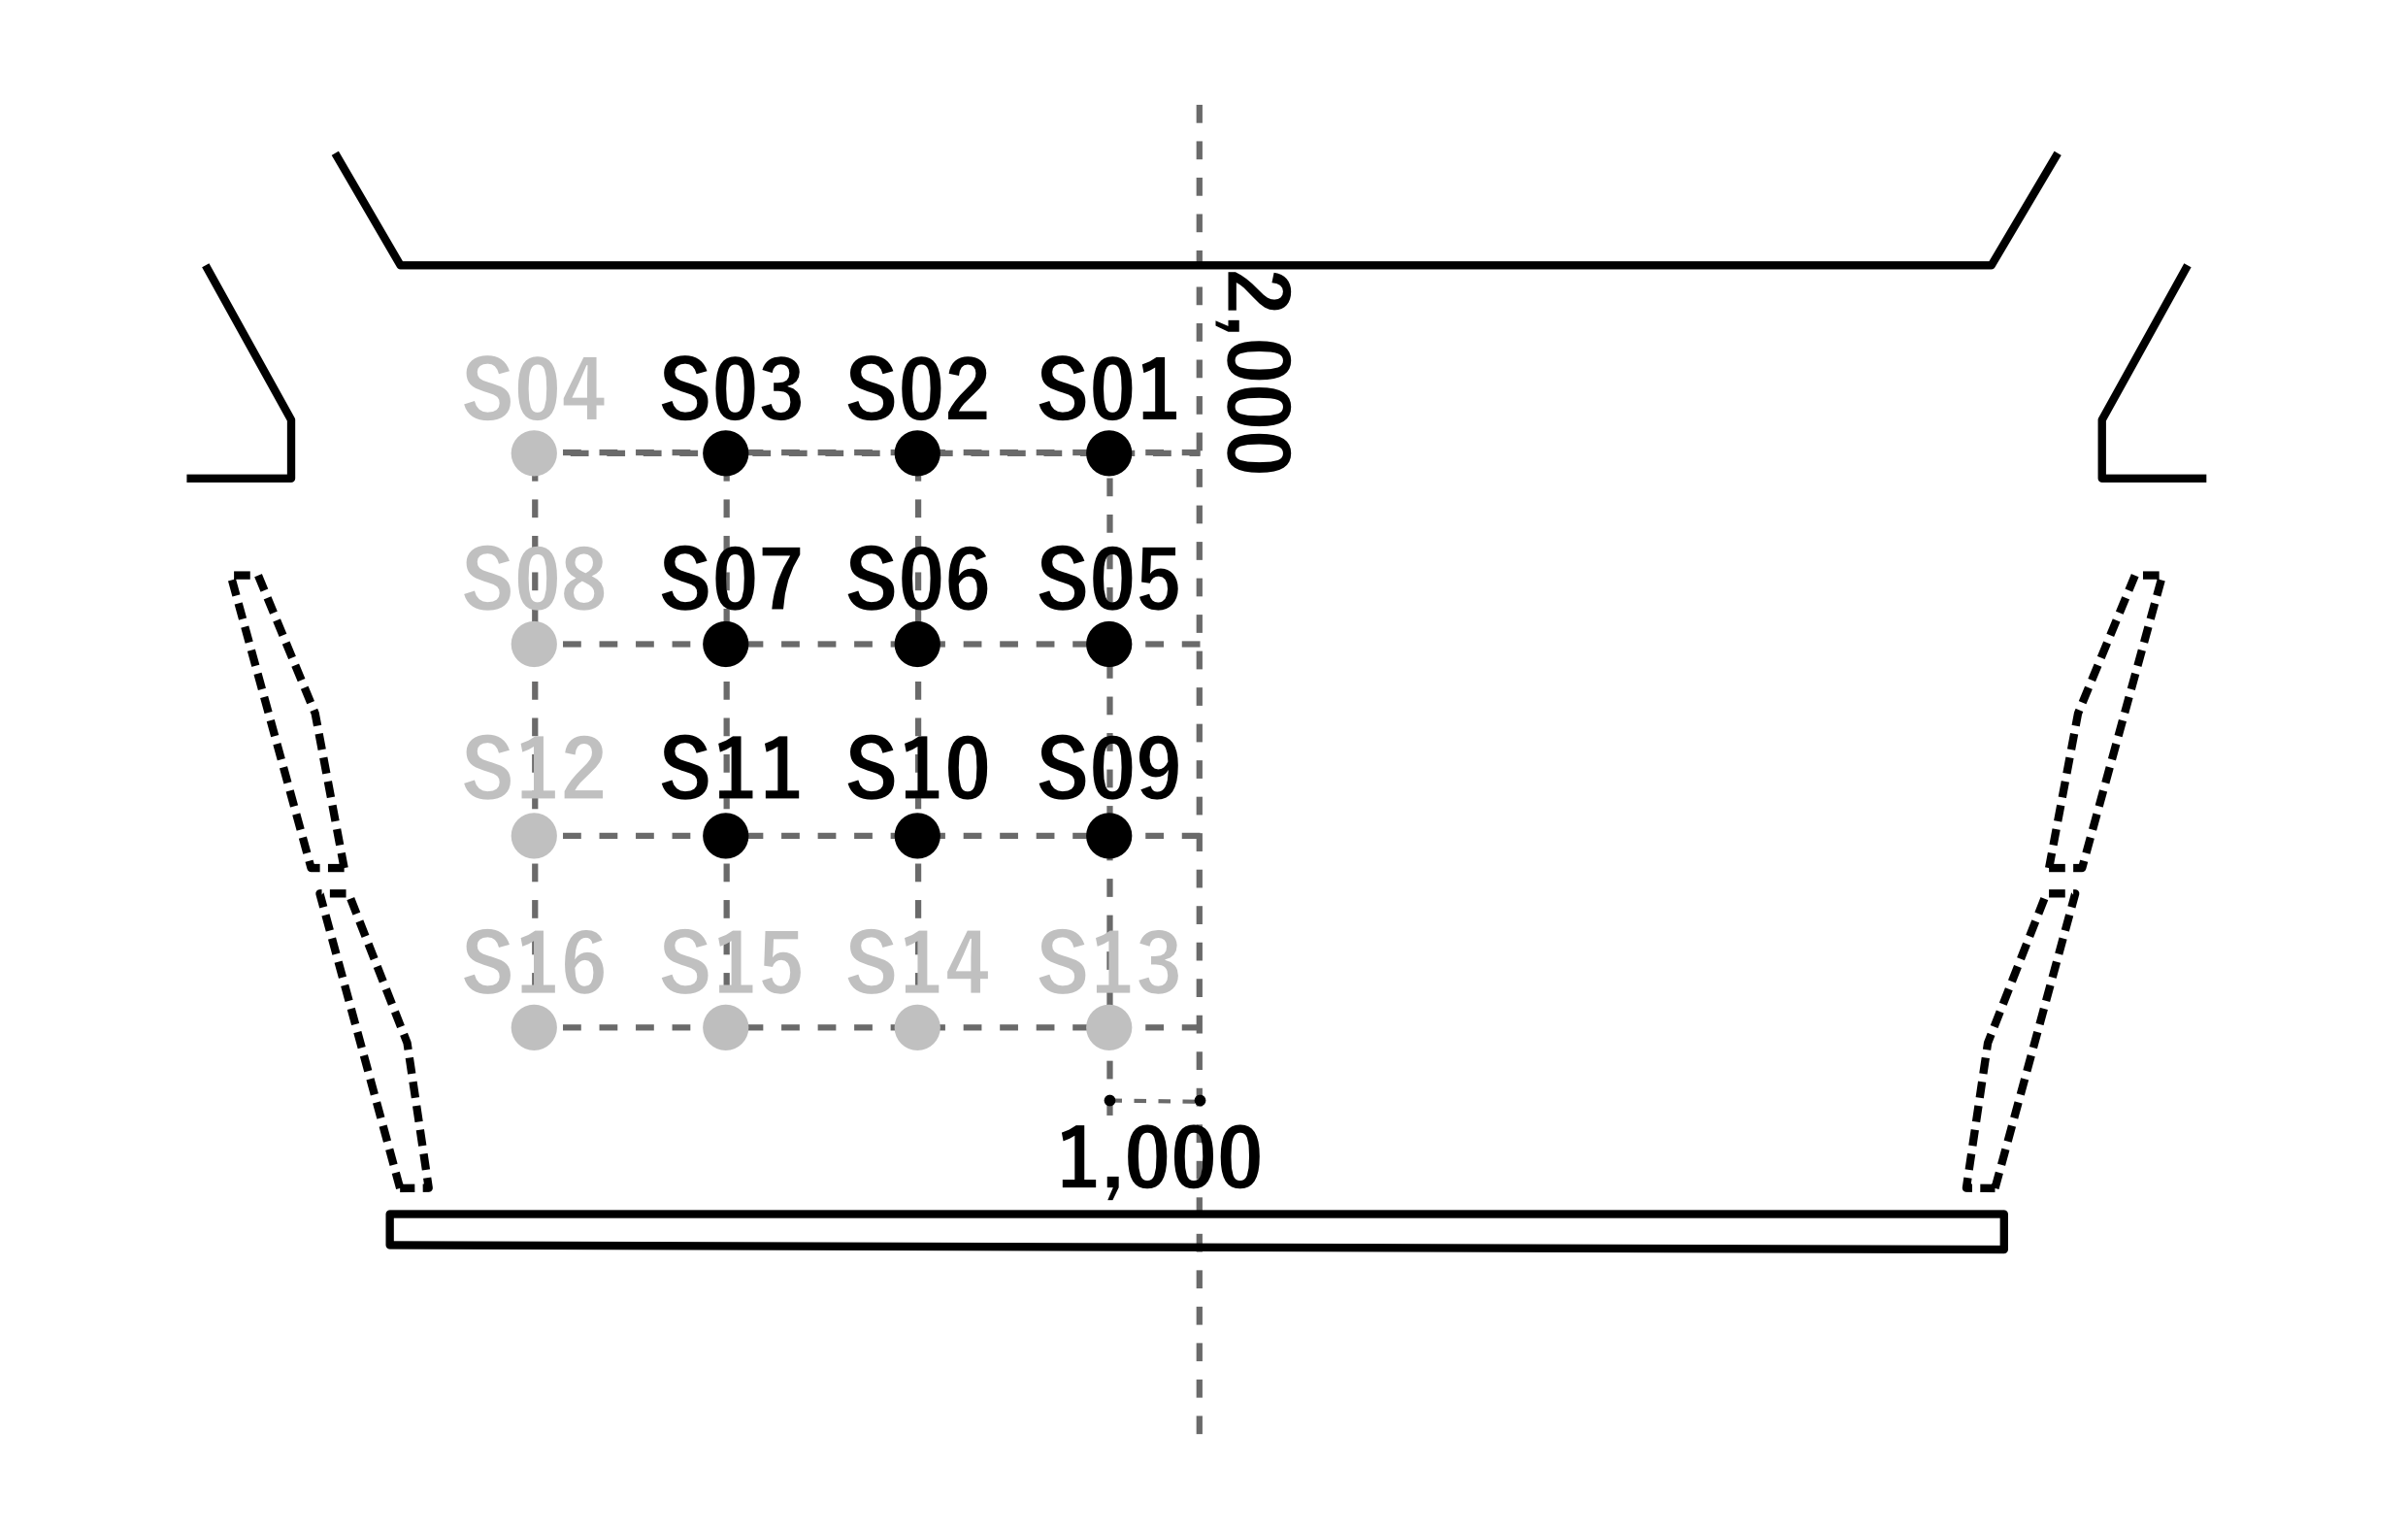
\includegraphics[width=.9\linewidth]{images/measuredHalls/flatud_hall_e.png}
    \caption*{ホールE}
  \end{minipage}%
  \begin{minipage}[b]{.5\textwidth}
    \centering
    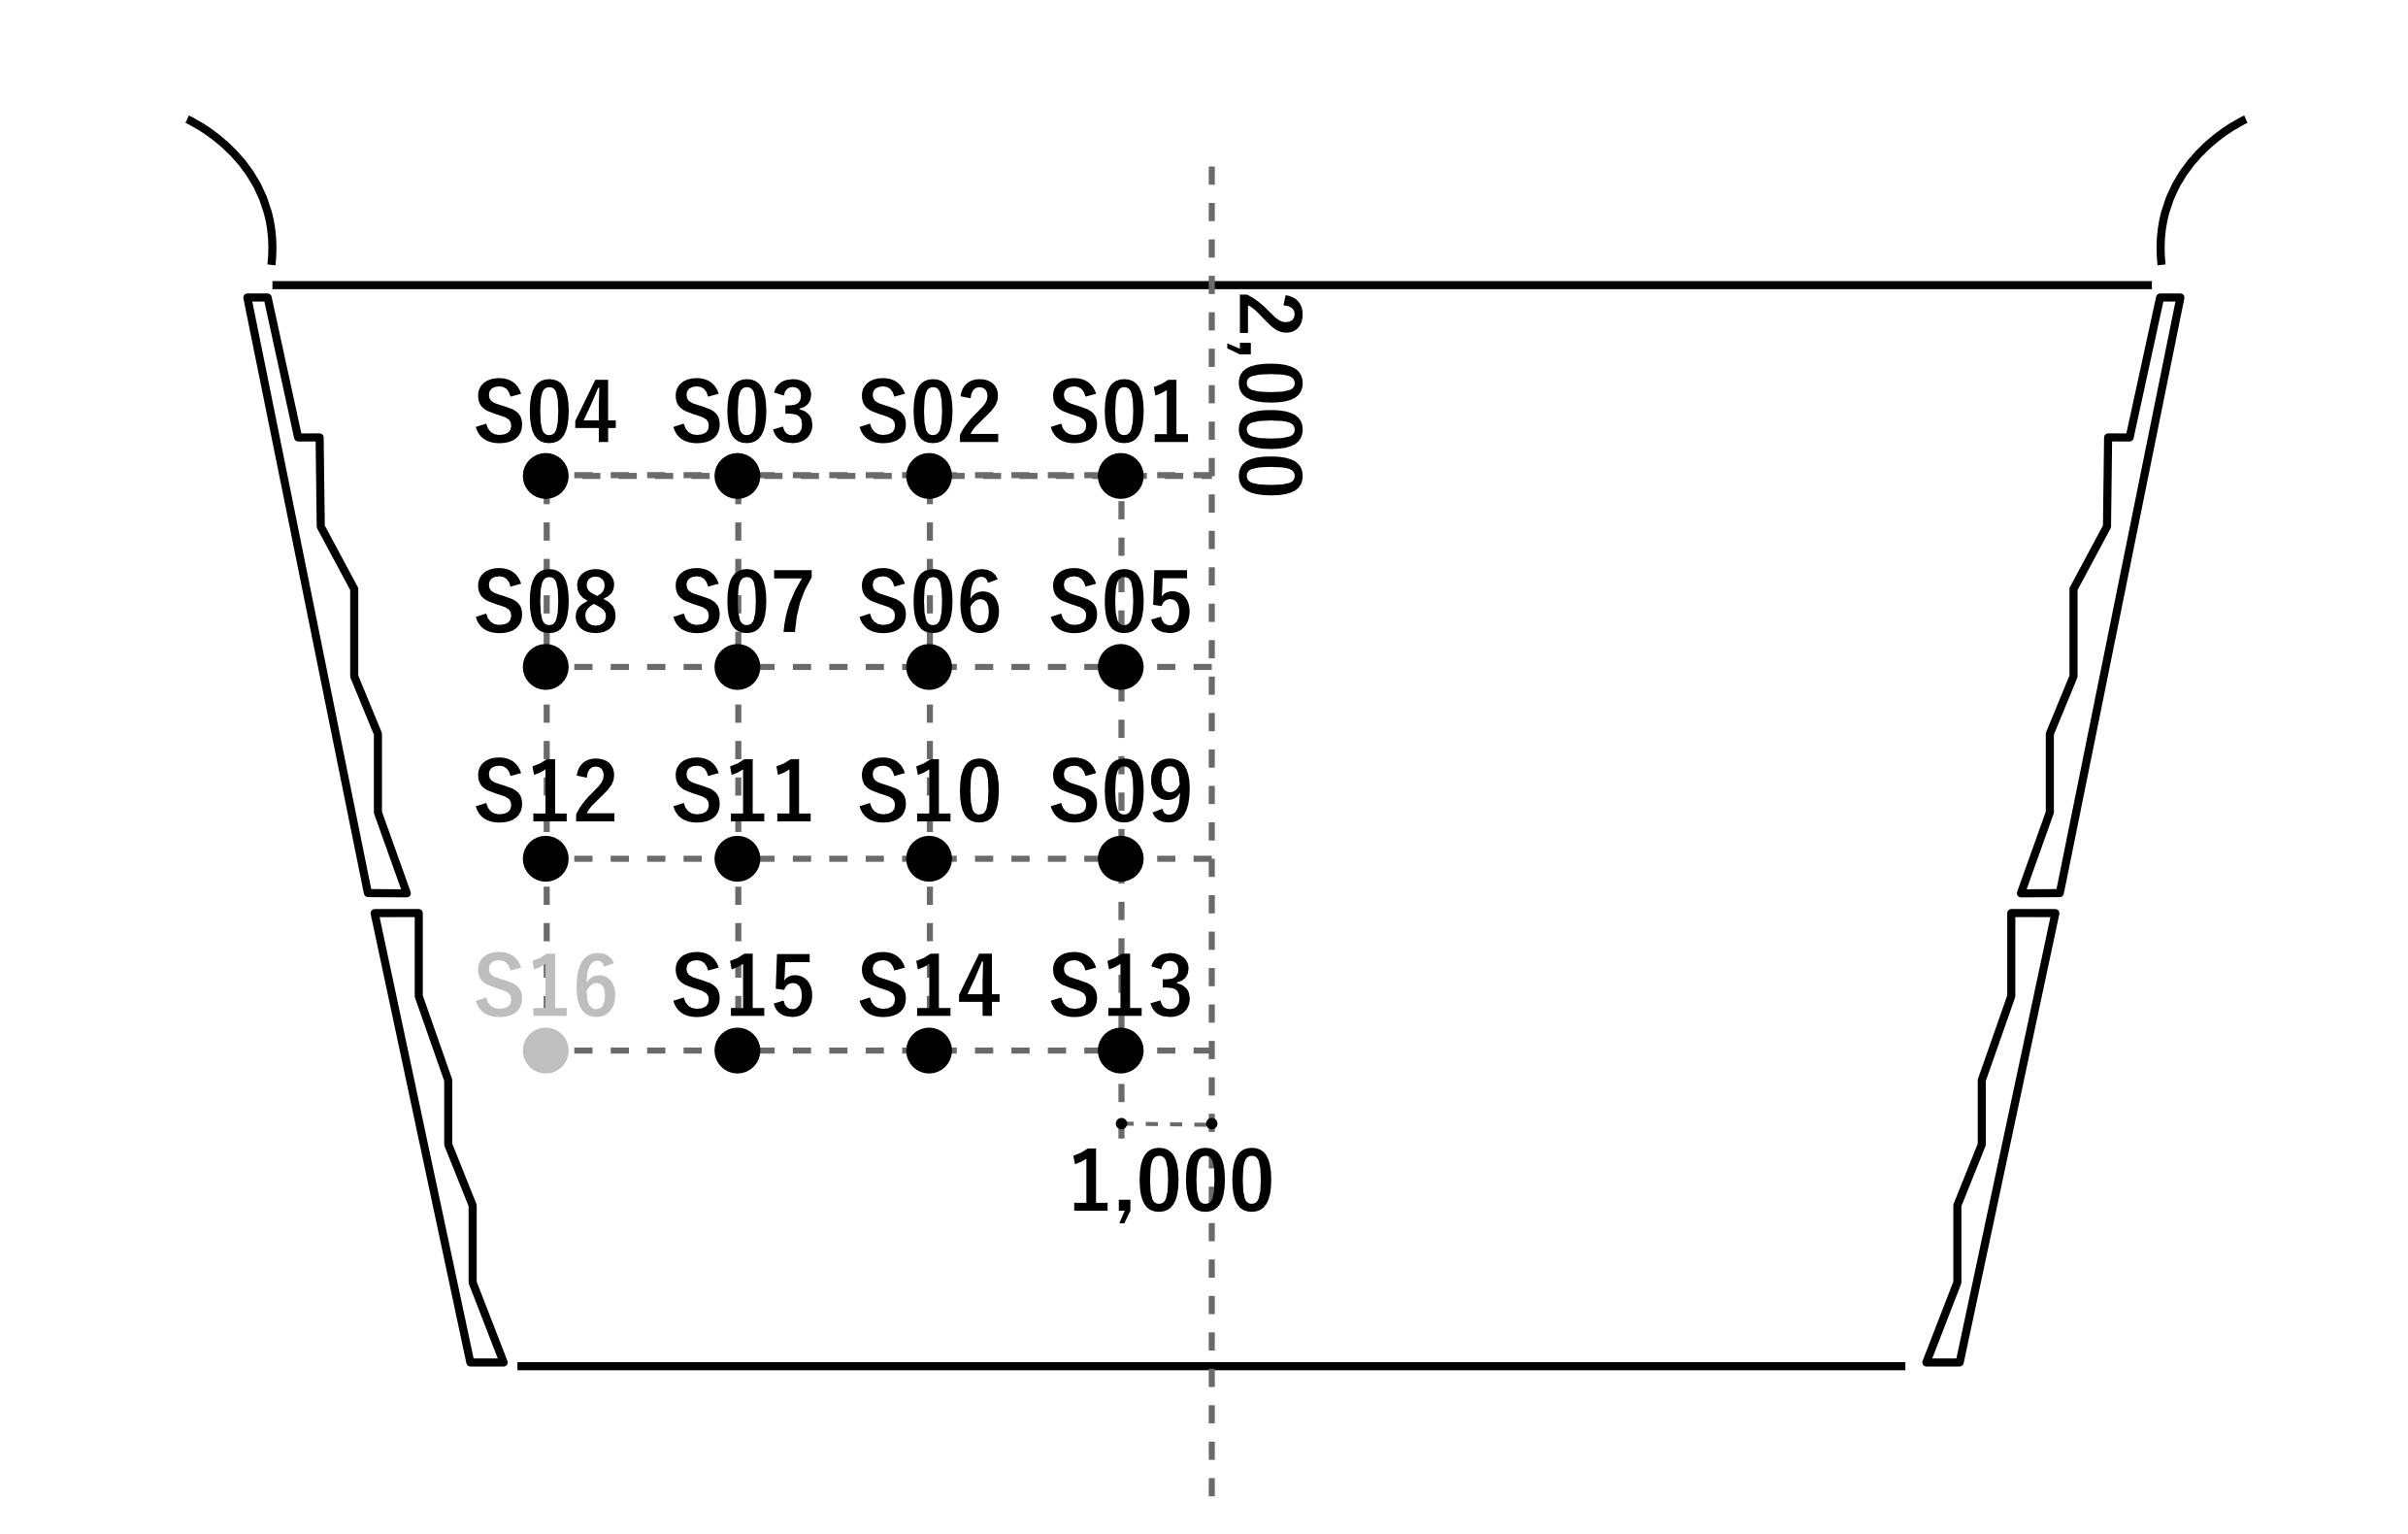
\includegraphics[width=.9\linewidth]{images/measuredHalls/flatud_hall_f.png}
    \caption*{ホールF}
  \end{minipage}

  \begin{minipage}[b]{1\textwidth}
    \centering
    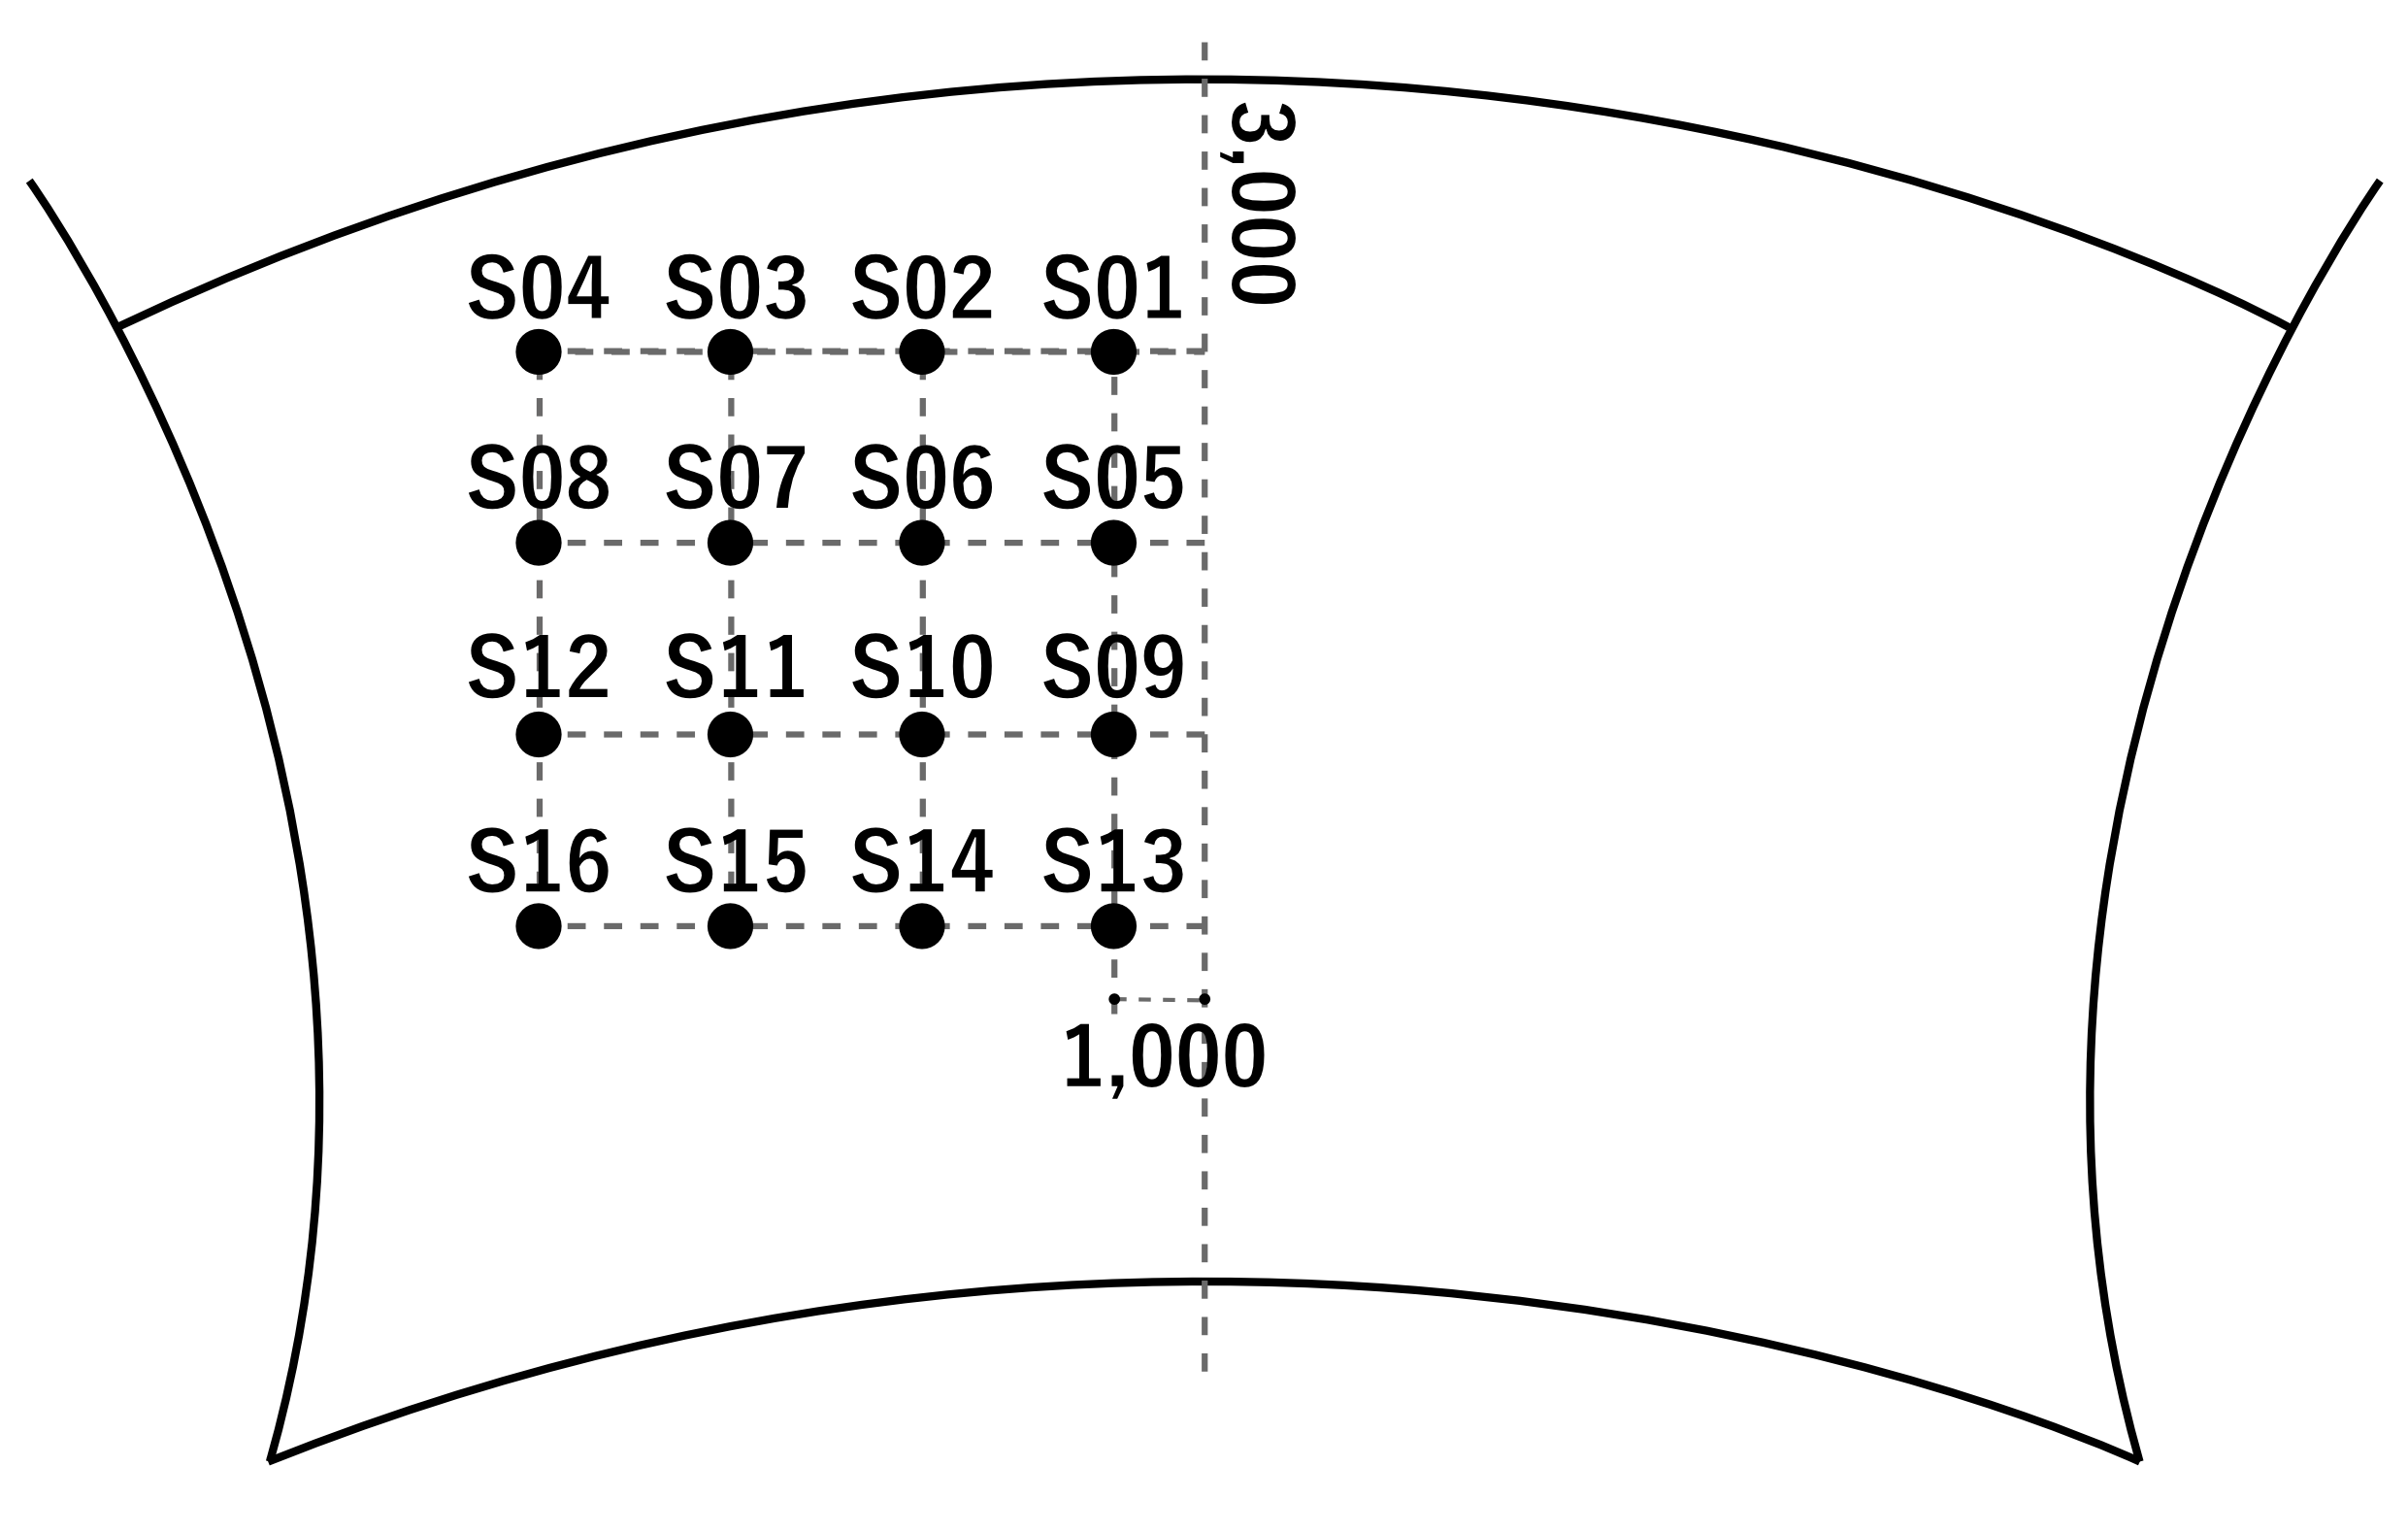
\includegraphics[width=.45\linewidth]{images/measuredHalls/flatud_hall_g.png}
    \caption*{ホールG}
  \end{minipage}

  \caption{各ホールの測定位置}
  \label{fig:各ホールの測定位置}
\end{figure}

%=======================================================================
% ホールA

\newpage
\begin{figure}[H]
  \begin{minipage}{.5\linewidth} % 右側の図
    \centering
    \includegraphics[width=.7\linewidth]{images/measuredHalls/resized/picture_a.jpg}
    \\ホールA 外観
  \end{minipage}%
  \begin{minipage}{.5\linewidth} % 右側の図
    \centering
    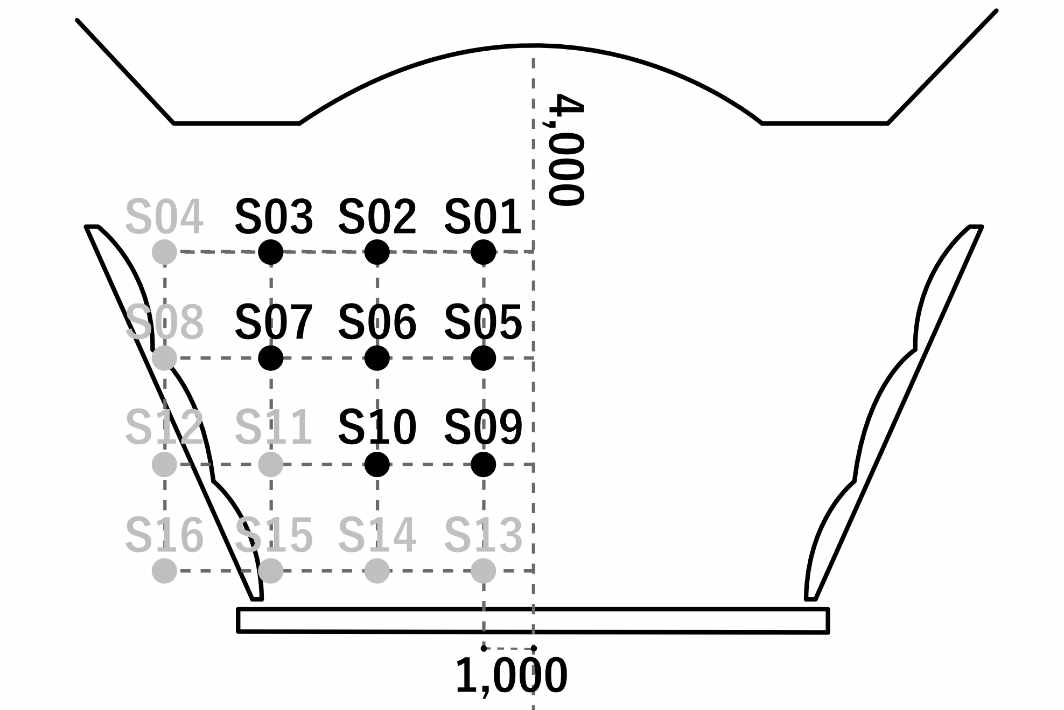
\includegraphics[width=.7\linewidth]{images/measuredHalls/resized/flat_a.jpg}
    \\ホールA 測定位置
  \end{minipage}

  \begin{minipage}{1\linewidth}
    \centering
    ホールA 諸元\\
    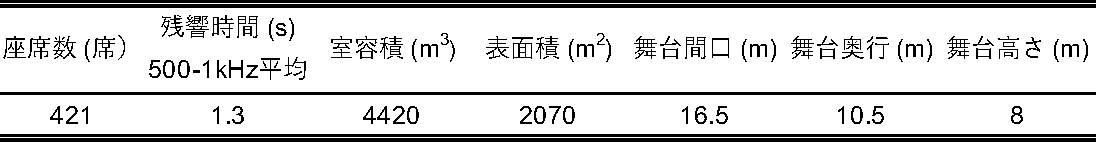
\includegraphics[width=.8\linewidth]{images/measuredHalls/informationTable/a.pdf}
  \end{minipage}
\end{figure}

\begin{figure}[H]
  \centering
  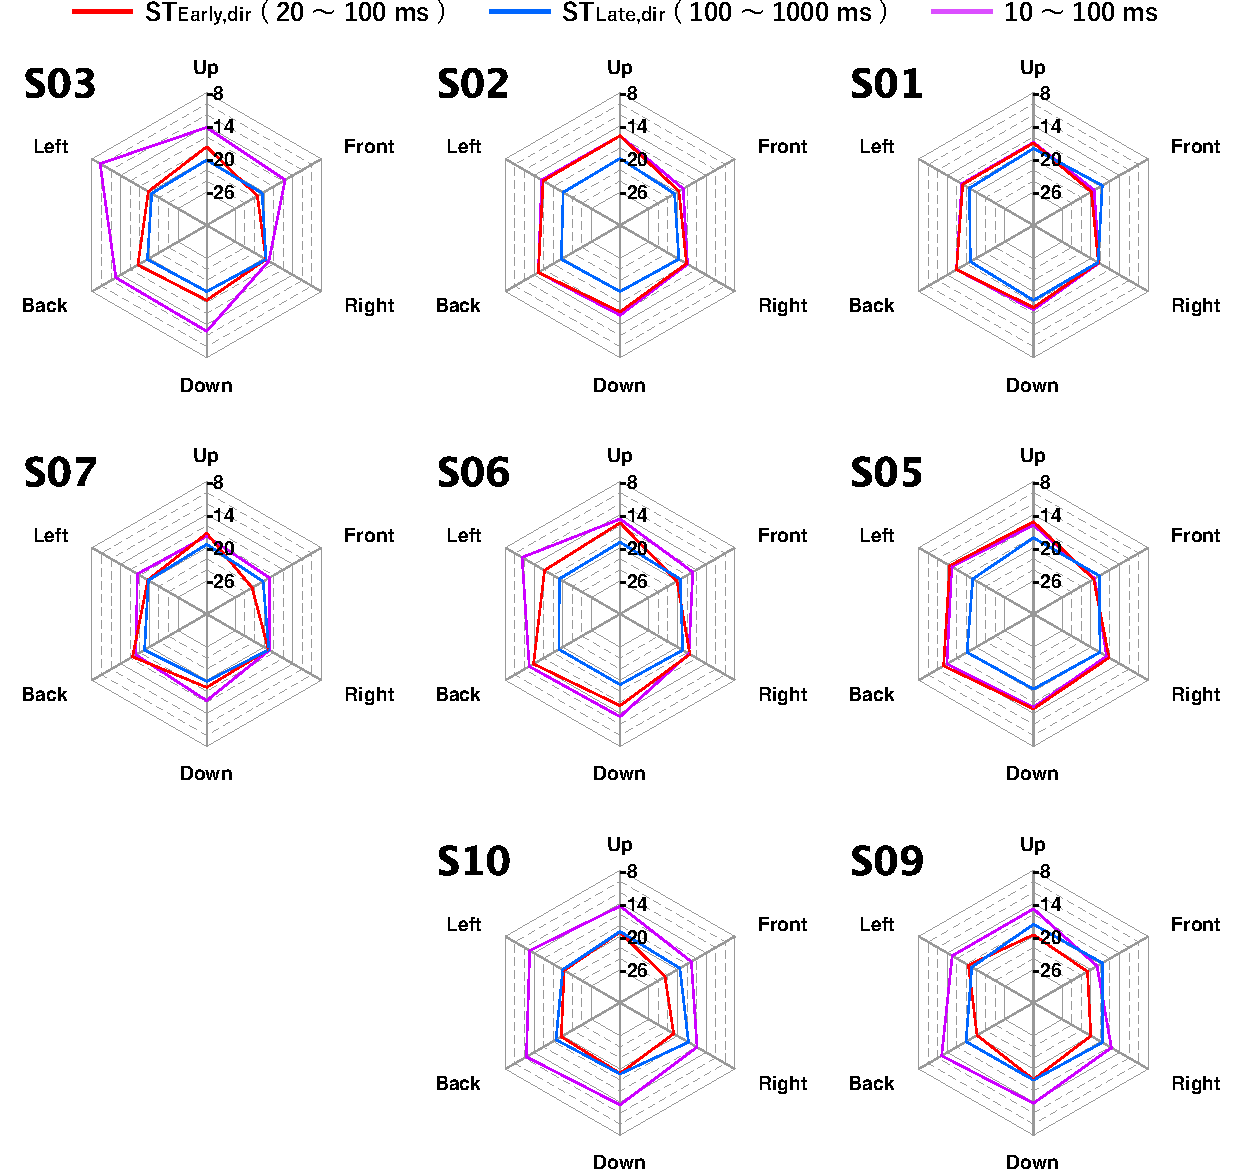
\includegraphics[scale=.75]{images/realHallDirSt/allPoint/reshaped/a.pdf}
  \caption{ホールA 方向別ST}
  \label{fig:ホールA 方向別ST}
\end{figure}

%=====================================================================
% ホールB
\newpage
\begin{figure}[H]
  \begin{minipage}{.5\linewidth} % 右側の図
    \centering
    \includegraphics[width=.7\linewidth]{images/measuredHalls/resized/picture_b.jpg}
    \\ホールB 外観
  \end{minipage}%
  \begin{minipage}{.5\linewidth} % 右側の図
    \centering
    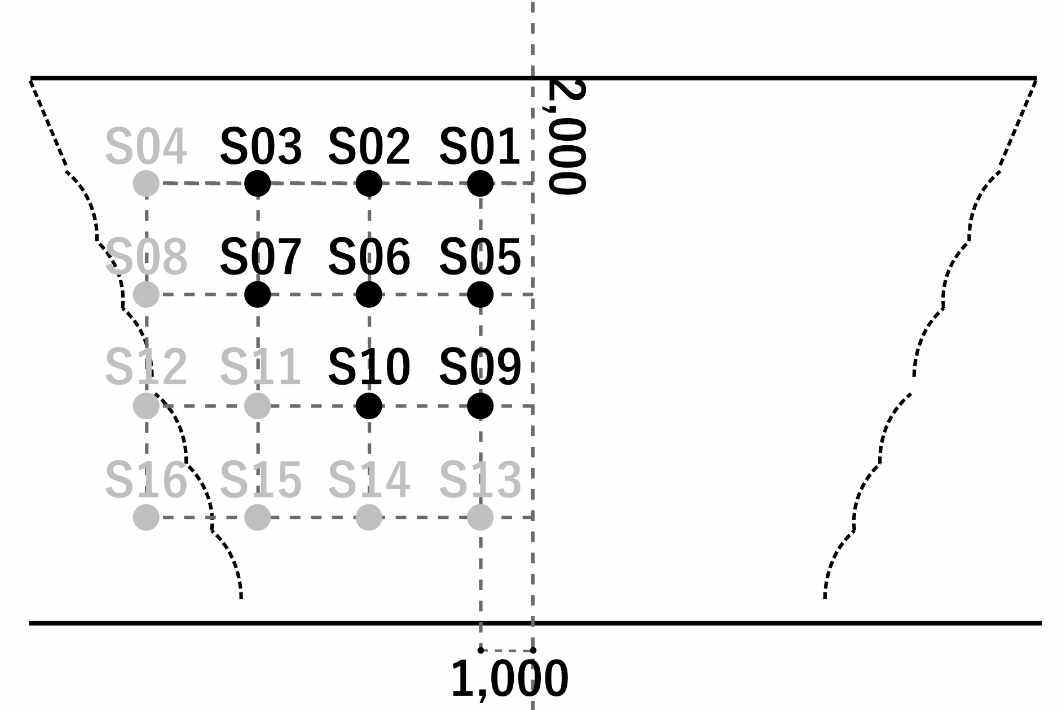
\includegraphics[width=.7\linewidth]{images/measuredHalls/resized/flat_b.jpg}
    \\ホールB 測定位置
  \end{minipage}

  \begin{minipage}{1\linewidth}
    \centering
    ホールB 諸元\\
    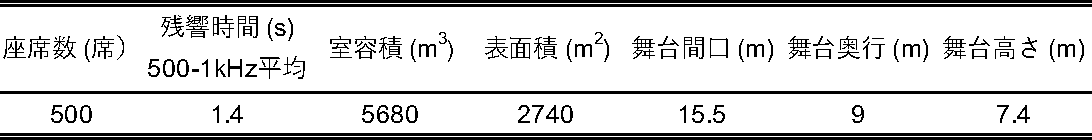
\includegraphics[width=.8\linewidth]{images/measuredHalls/informationTable/b.pdf}
  \end{minipage}
\end{figure}

\begin{figure}[H]
  \centering
  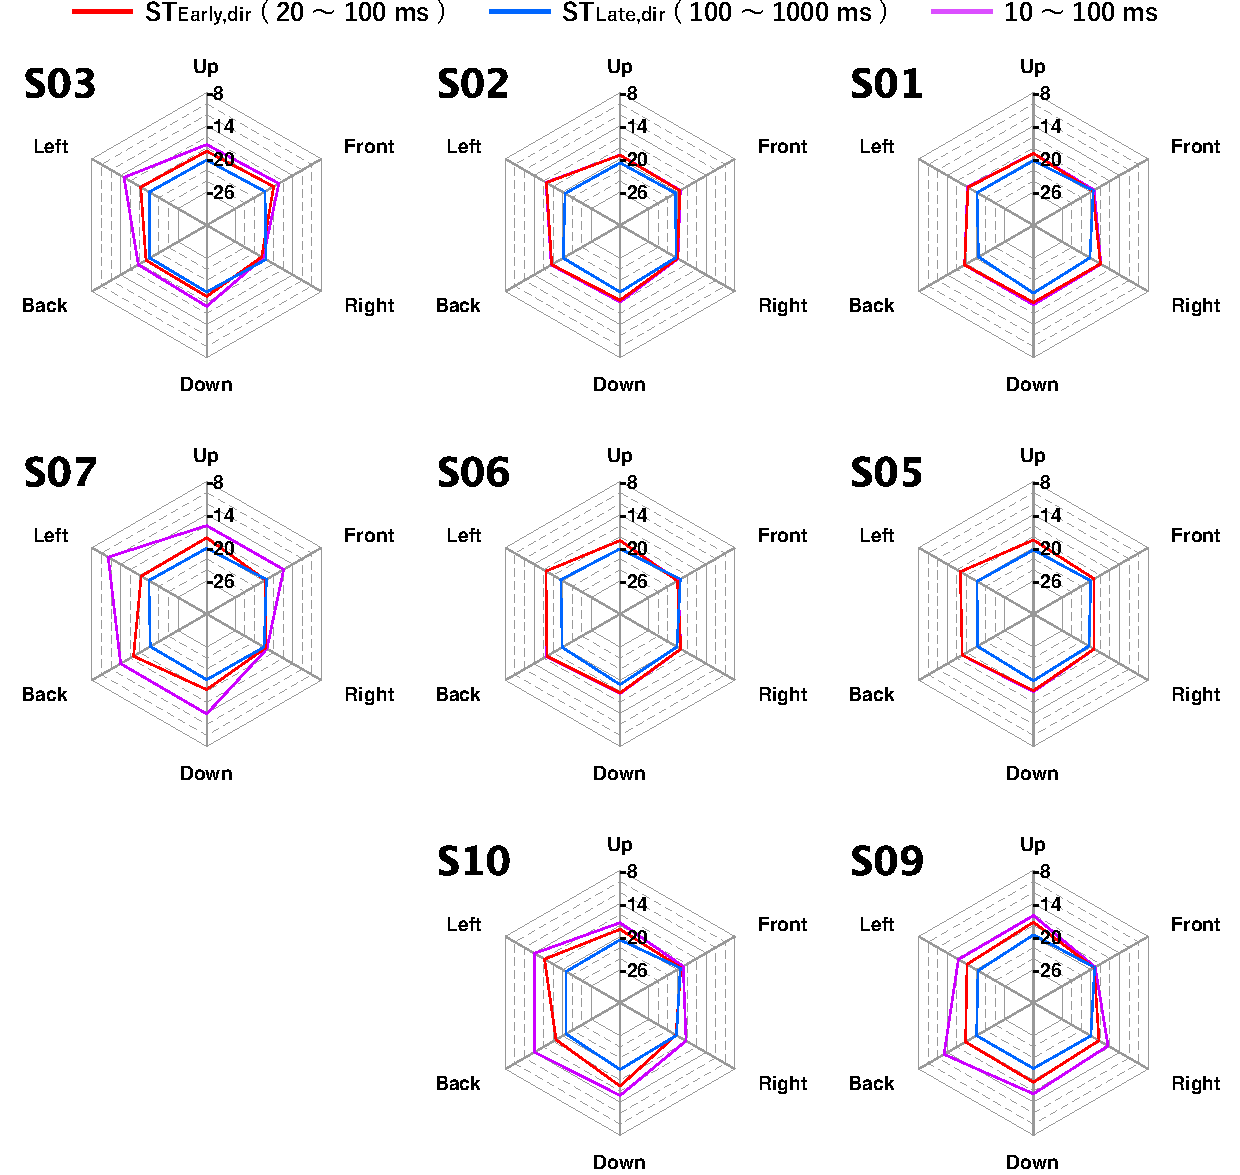
\includegraphics[scale=.75]{images/realHallDirSt/allPoint/reshaped/b.pdf}
  \caption{ホールB 方向別ST}
  \label{fig:ホールB 方向別ST}
\end{figure}

%=====================================================================
% ホールC
\newpage
\vspace*{6\baselineskip}

\begin{figure}[H]
  \begin{minipage}{.5\linewidth}
    \centering
    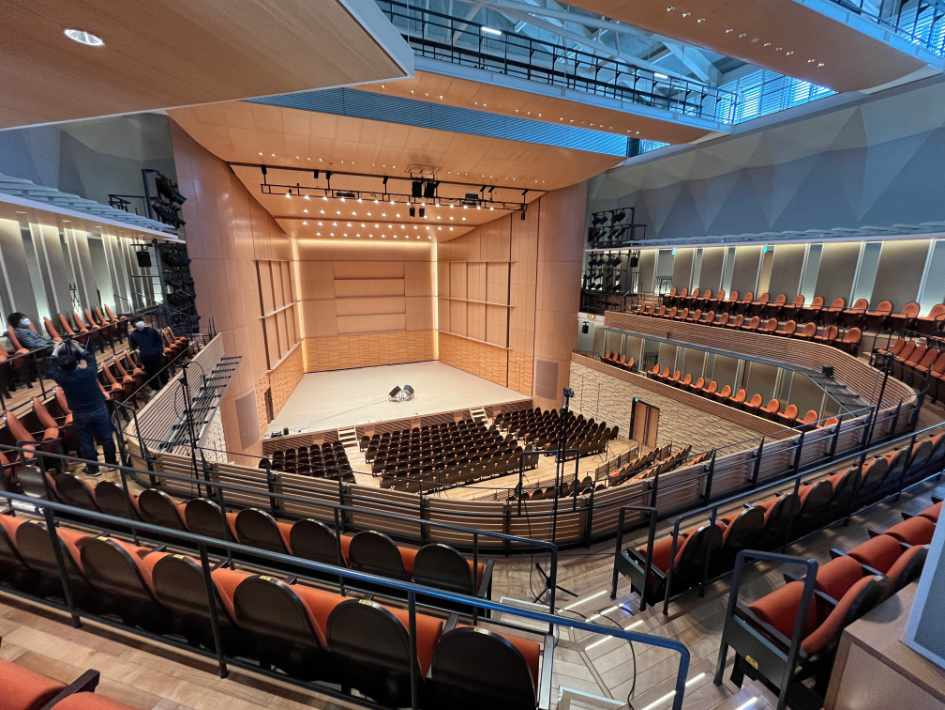
\includegraphics[width=.7\linewidth]{images/measuredHalls/resized/picture_c.jpg}
    \caption*{ホールC 外観}  
  \end{minipage}%
  \begin{minipage}{.5\linewidth}
    \centering
    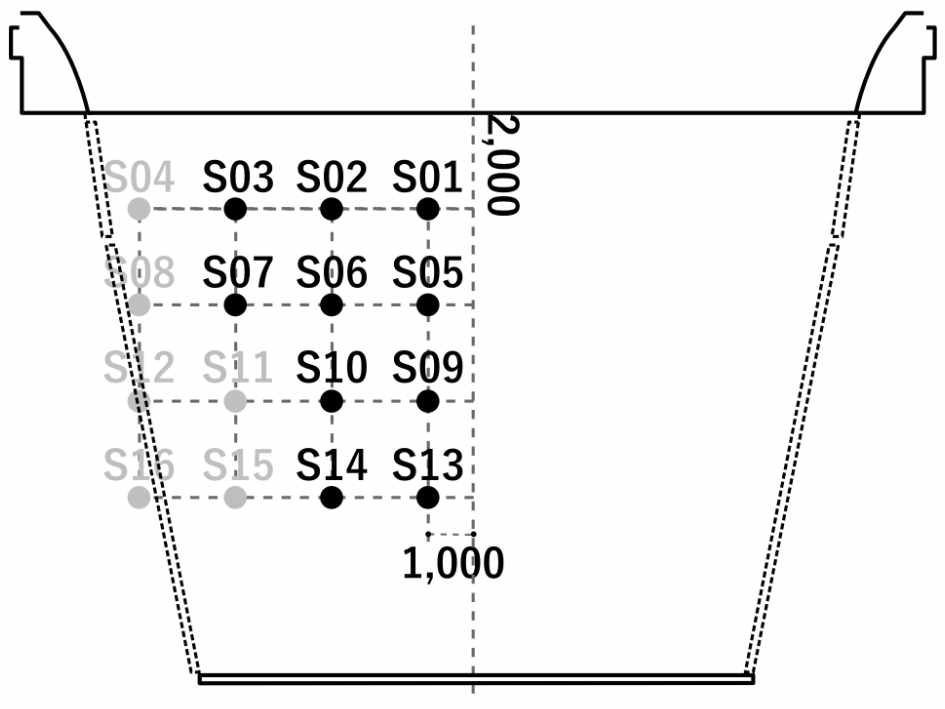
\includegraphics[width=.7\linewidth]{images/measuredHalls/resized/flat_c.jpg}
    \caption*{ホールC 測定位置}
  \end{minipage}
\end{figure}

\vspace{2\baselineskip}

\begin{table}[H]
  \centering
  \caption*{ホールC 諸元}
  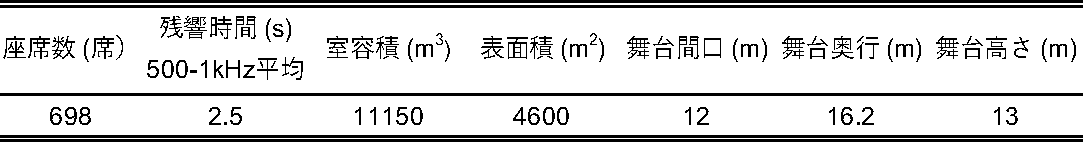
\includegraphics[width=.8\linewidth]{images/measuredHalls/informationTable/c_wide.pdf}
\end{table}

\newpage
\begin{figure}[H]
  \centering
  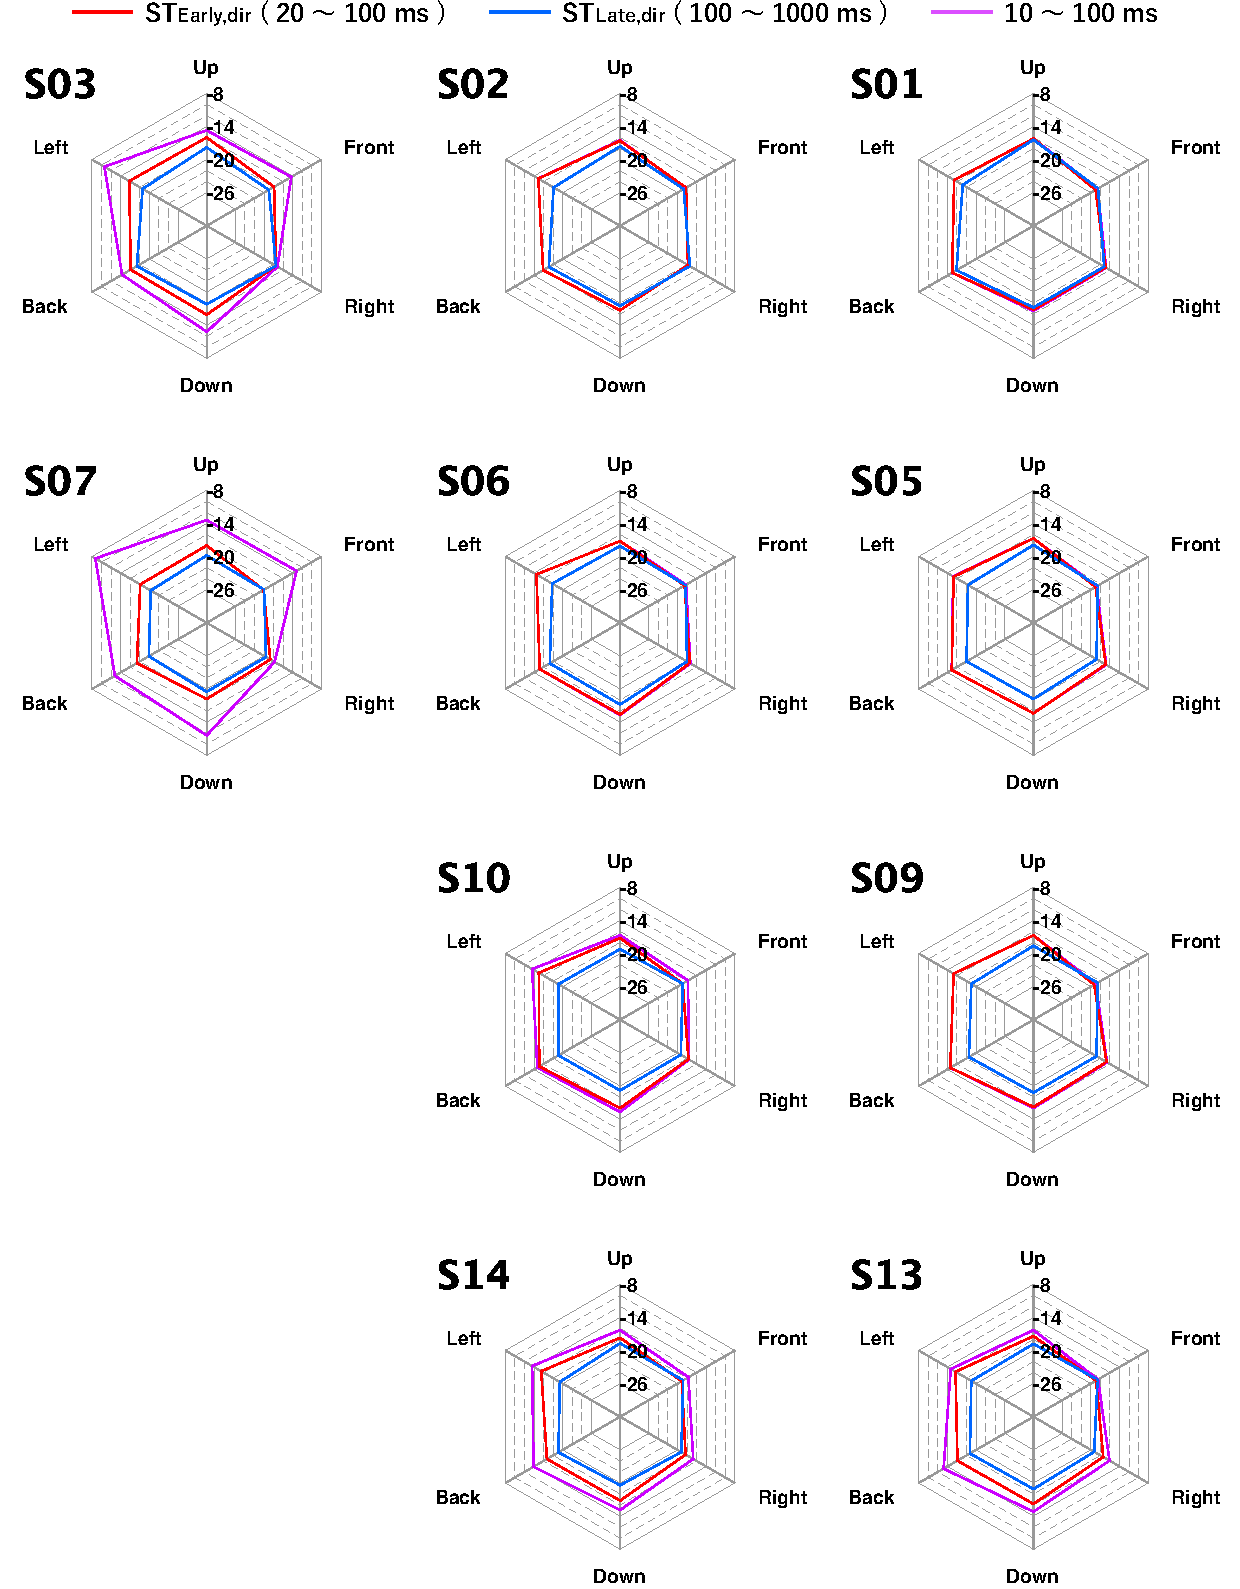
\includegraphics[scale=.75]{images/realHallDirSt/allPoint/reshaped/c.pdf}
  \caption{ホールC 方向別ST}
  \label{fig:ホールC 方向別ST}
\end{figure}

%=====================================================================
% ホールD
\newpage
\begin{figure}[H]
  \begin{minipage}{.5\linewidth} % 右側の図
    \centering
    \includegraphics[width=.7\linewidth]{images/measuredHalls/resized/picture_d.jpg}
    \\ホールD 外観
  \end{minipage}%
  \begin{minipage}{.5\linewidth} % 右側の図
    \centering
    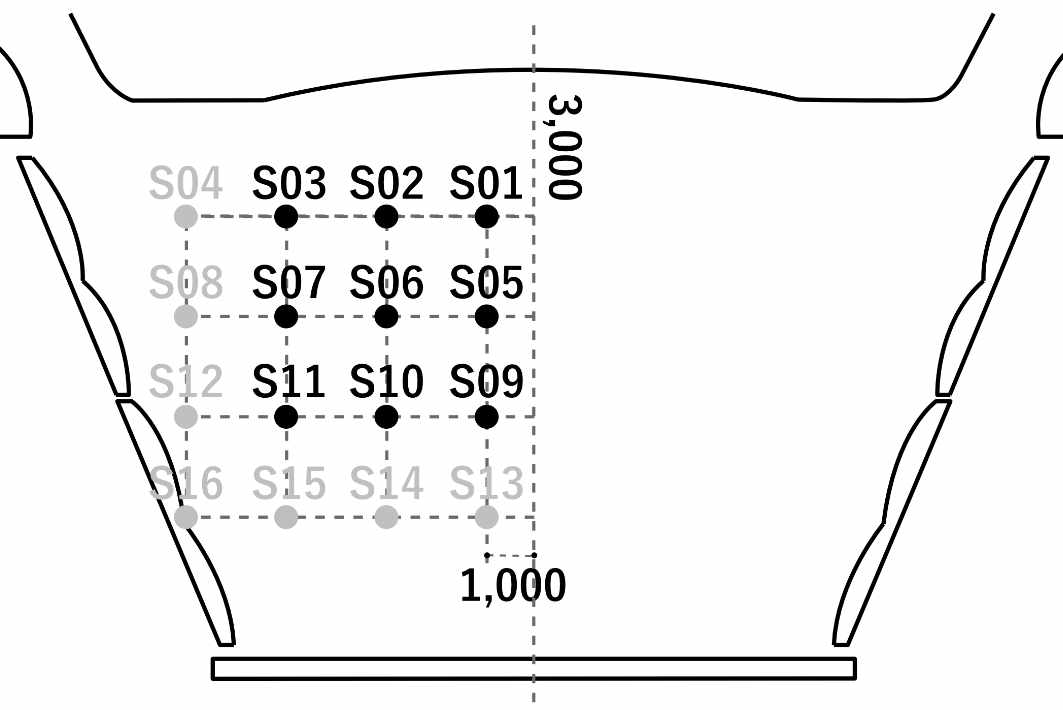
\includegraphics[width=.7\linewidth]{images/measuredHalls/resized/flat_d.jpg}
    \\ホールD 測定位置
  \end{minipage}

  \begin{minipage}{1\linewidth}
    \centering
    ホールD 諸元\\
    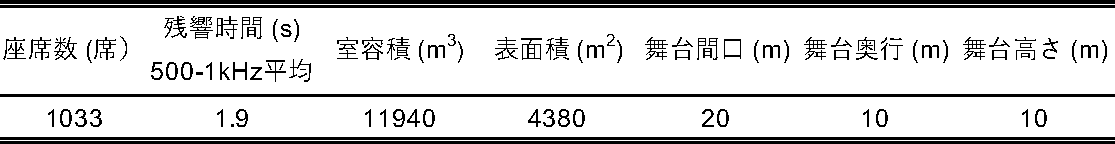
\includegraphics[width=.8\linewidth]{images/measuredHalls/informationTable/d.pdf}
  \end{minipage}
\end{figure}

\begin{figure}[H]
  \centering
  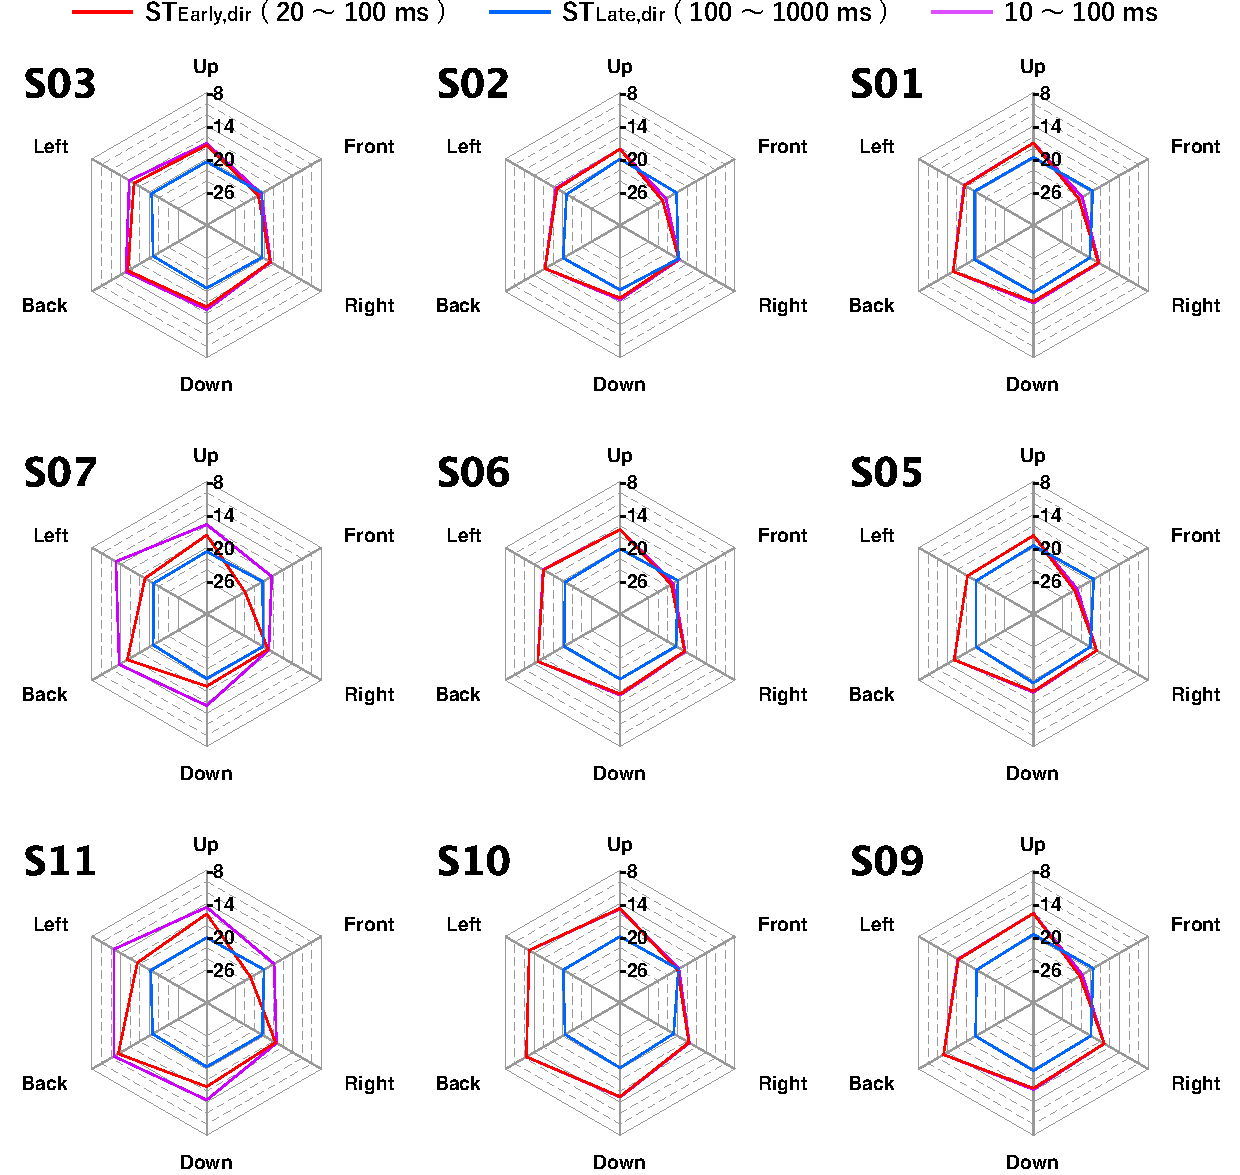
\includegraphics[scale=.77]{images/realHallDirSt/allPoint/reshaped/d.pdf}
  \caption{ホールD 方向別ST}
  \label{fig:ホールD 方向別ST}
\end{figure}

%=====================================================================
% ホールE
\newpage
\begin{figure}[H]
  \begin{minipage}{.5\linewidth} % 右側の図
    \centering
    \includegraphics[width=.7\linewidth]{images/measuredHalls/resized/picture_e.jpg}
    \\ホールE 外観
  \end{minipage}%
  \begin{minipage}{.5\linewidth} % 右側の図
    \centering
    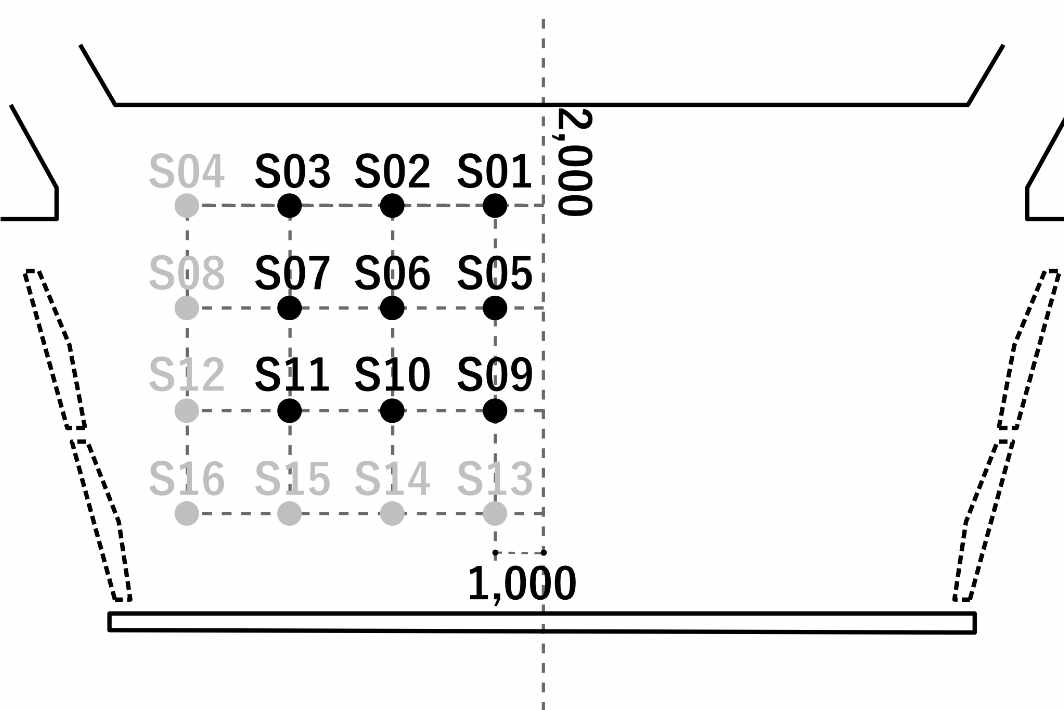
\includegraphics[width=.7\linewidth]{images/measuredHalls/resized/flat_e.jpg}
    \\ホールE 測定位置
  \end{minipage}

  \begin{minipage}{1\linewidth}
    \centering
    ホールE 諸元\\
    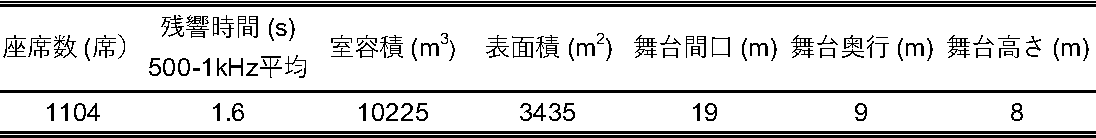
\includegraphics[width=.8\linewidth]{images/measuredHalls/informationTable/e.pdf}
  \end{minipage}
\end{figure}

\begin{figure}[H]
  \centering
  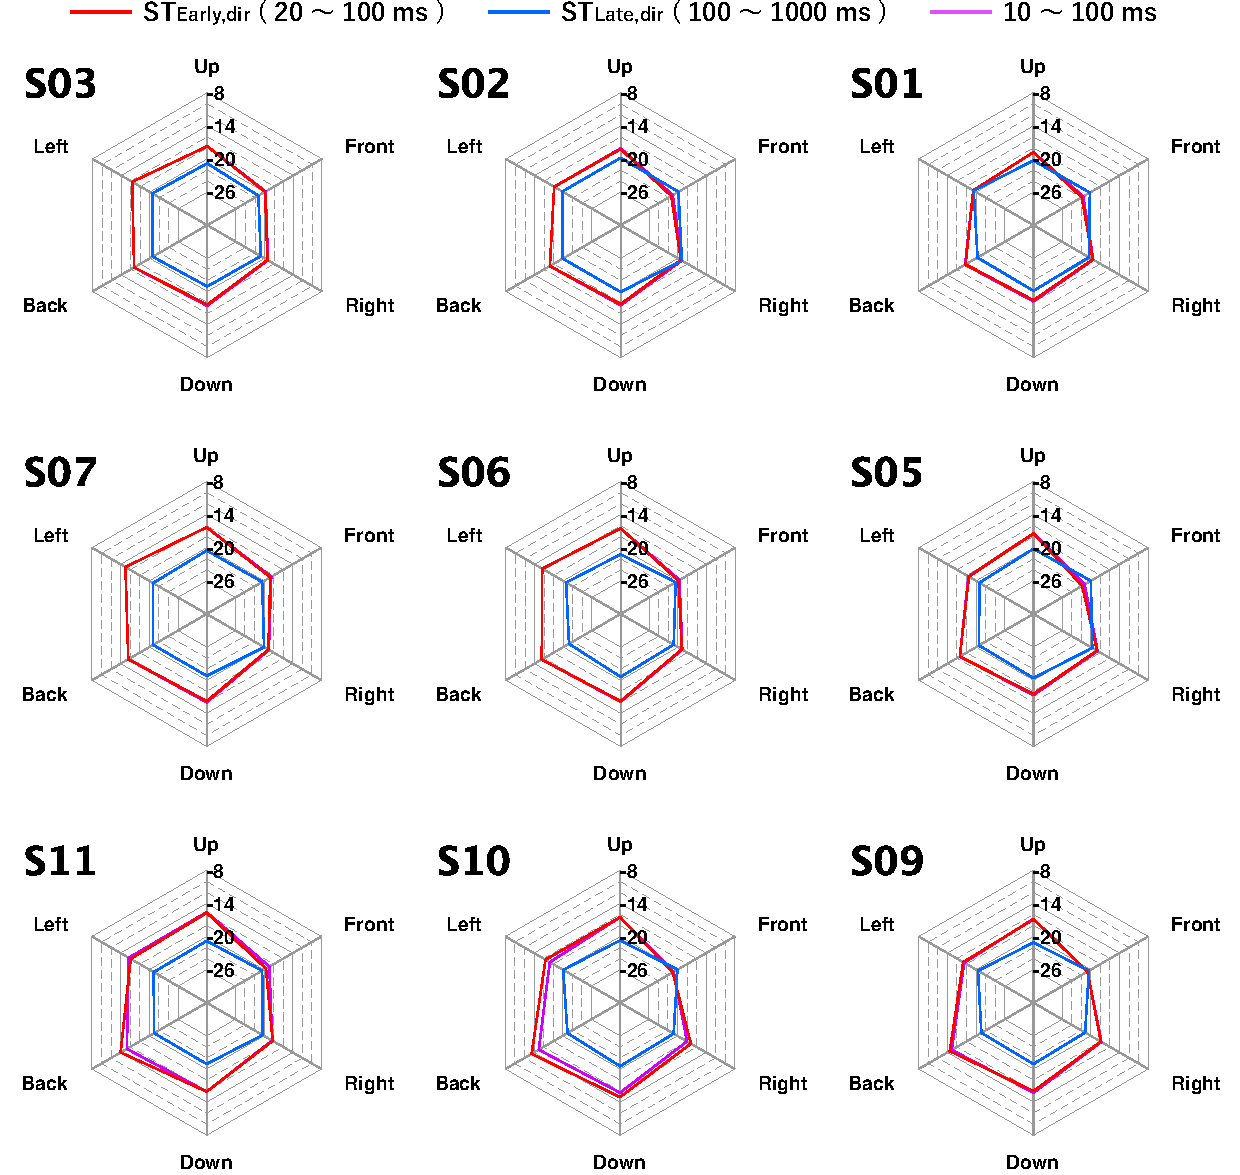
\includegraphics[scale=.77]{images/realHallDirSt/allPoint/reshaped/e.pdf}
  \caption{ホールE 方向別ST}
  \label{fig:ホールE 方向別ST}
\end{figure}

%=====================================================================
\newpage
\vspace{4\baselineskip}

\begin{figure}[H]
  \begin{minipage}{0.5\textwidth} % 左側の図
    \centering
    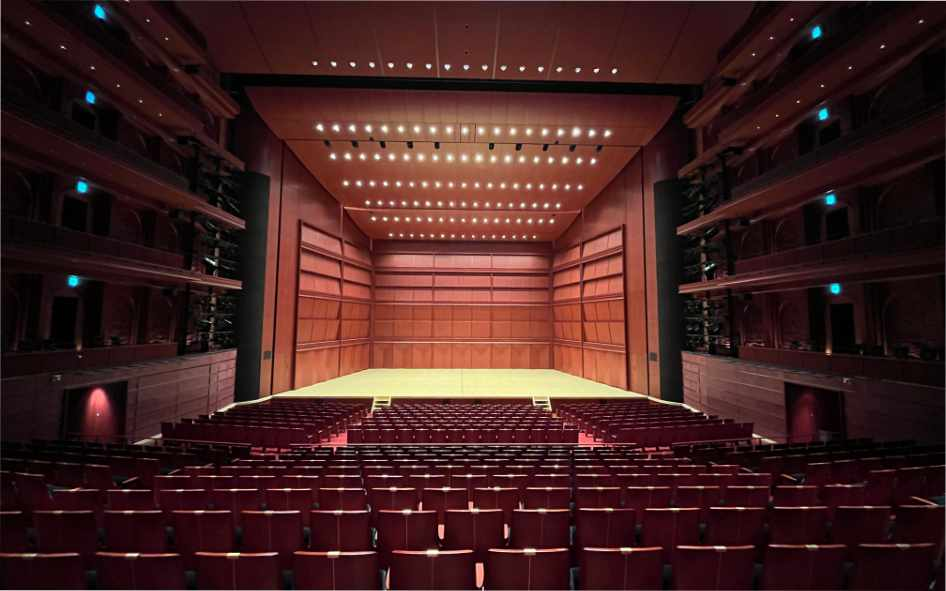
\includegraphics[width=.8\linewidth]{images/measuredHalls/resized/picture_f.jpg}
    \\ホールF 外観
    \vspace{2\baselineskip}

    ホールF 諸元\\
    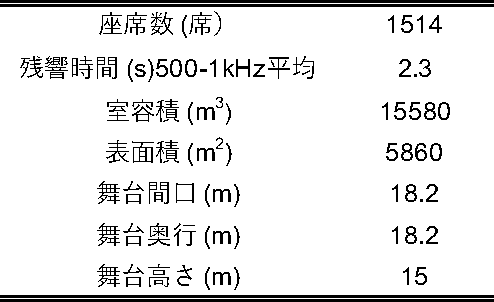
\includegraphics[width=.8\linewidth]{images/measuredHalls/informationTable/f.pdf}
    \vspace{2\baselineskip}

    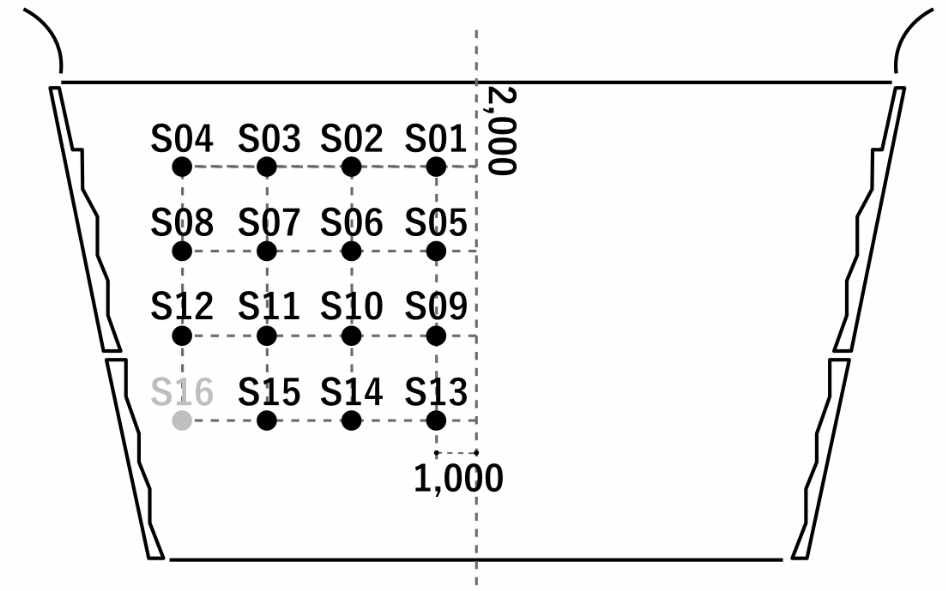
\includegraphics[width=.8\linewidth]{images/measuredHalls/resized/flat_f.jpg}
    \\ホールF 測定位置
  \end{minipage}%
  \begin{minipage}{.5\linewidth} % 右側の図
    \raggedleft
    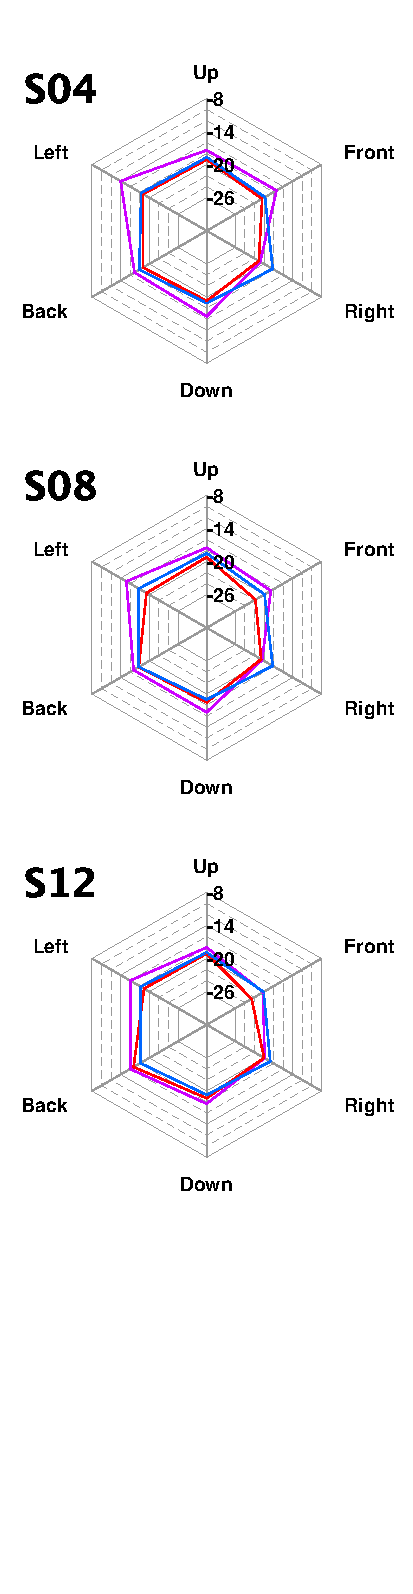
\includegraphics[scale=.77]{images/realHallDirSt/allPoint/reshaped/fLeftPage.pdf}
  \end{minipage}
\end{figure}

\newpage

\begin{figure}[H]
  \centering
  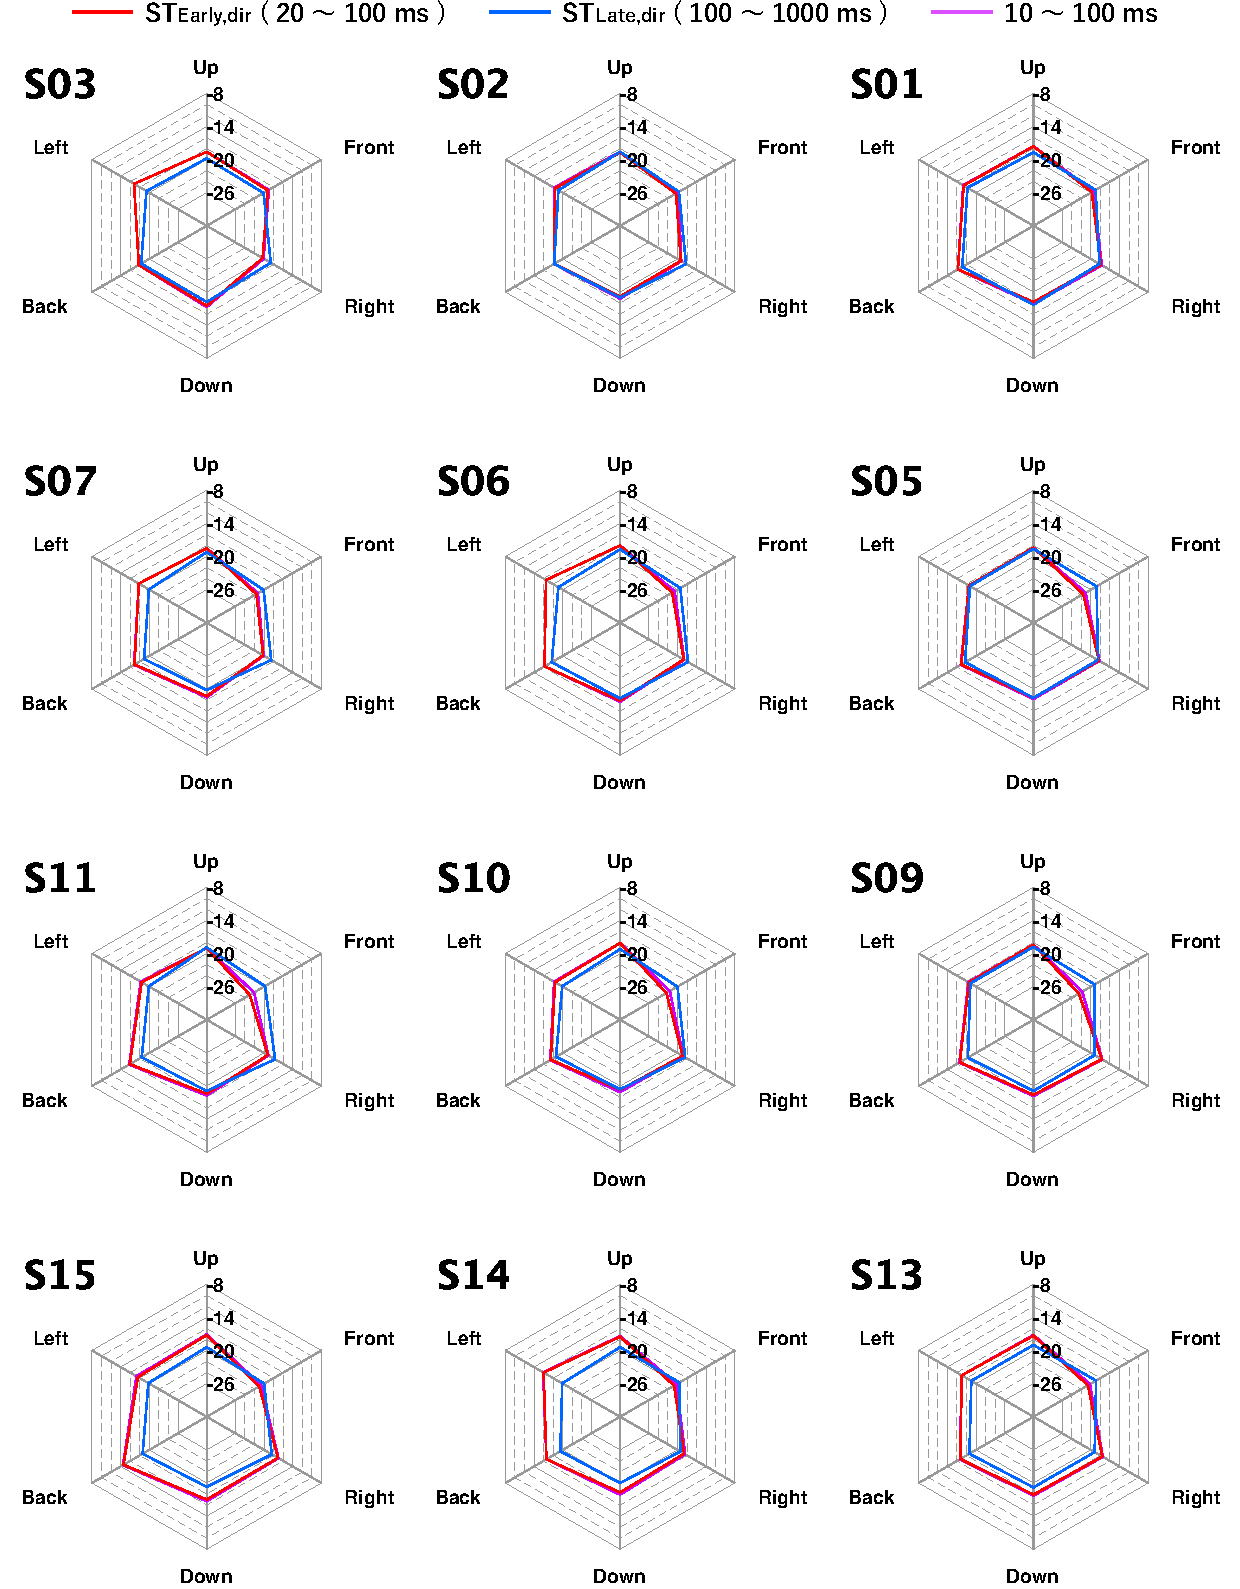
\includegraphics[scale=.77]{images/realHallDirSt/allPoint/reshaped/fRightPage.pdf}
  \caption{ホールF 方向別ST}
  \label{fig:ホールF 方向別ST}
\end{figure}

%=======================================================================
\newpage
  
\vspace{4\baselineskip}

\begin{figure}[H]
  \begin{minipage}{0.5\textwidth} % 左側の図
    \centering

    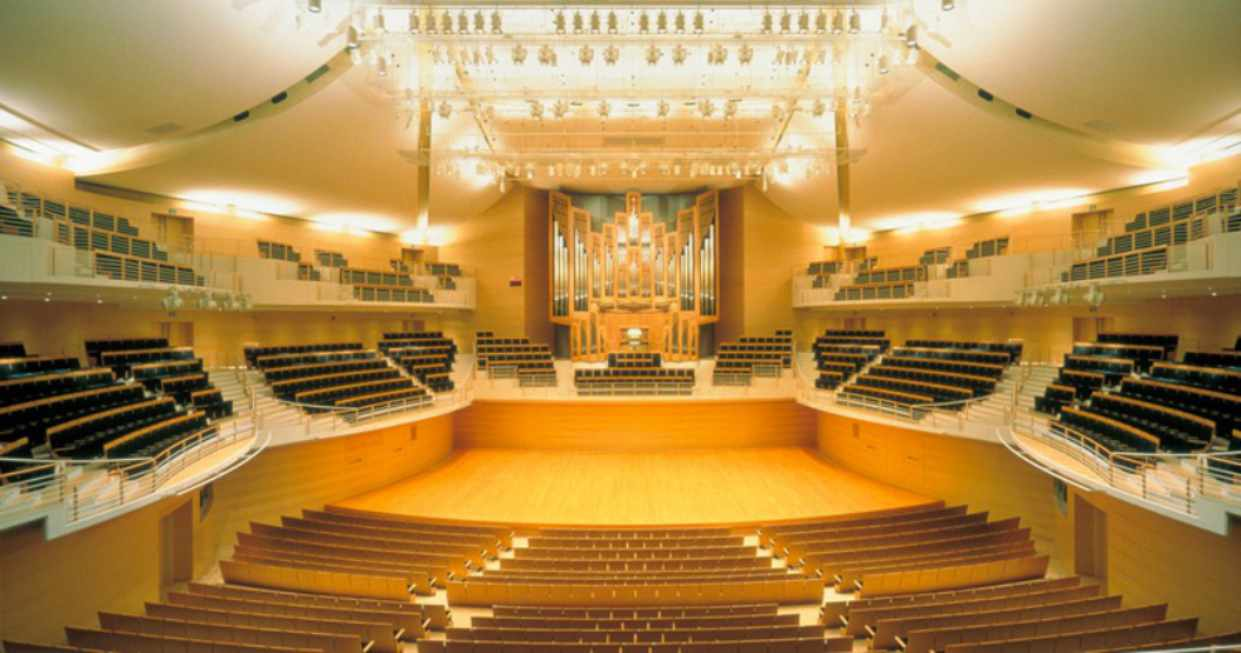
\includegraphics[width=.8\linewidth]{images/measuredHalls/resized/picture_g.jpg}
    \\ホールG 外観
    \vspace{2\baselineskip}

    ホールG 諸元\\
    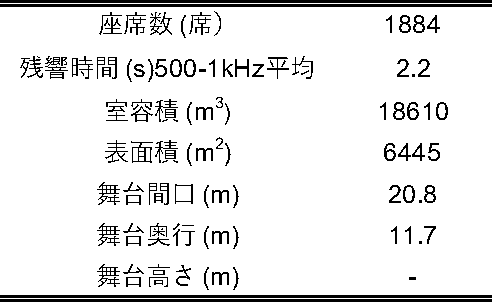
\includegraphics[width=.8\linewidth]{images/measuredHalls/informationTable/g.pdf}
    \vspace{2\baselineskip}

    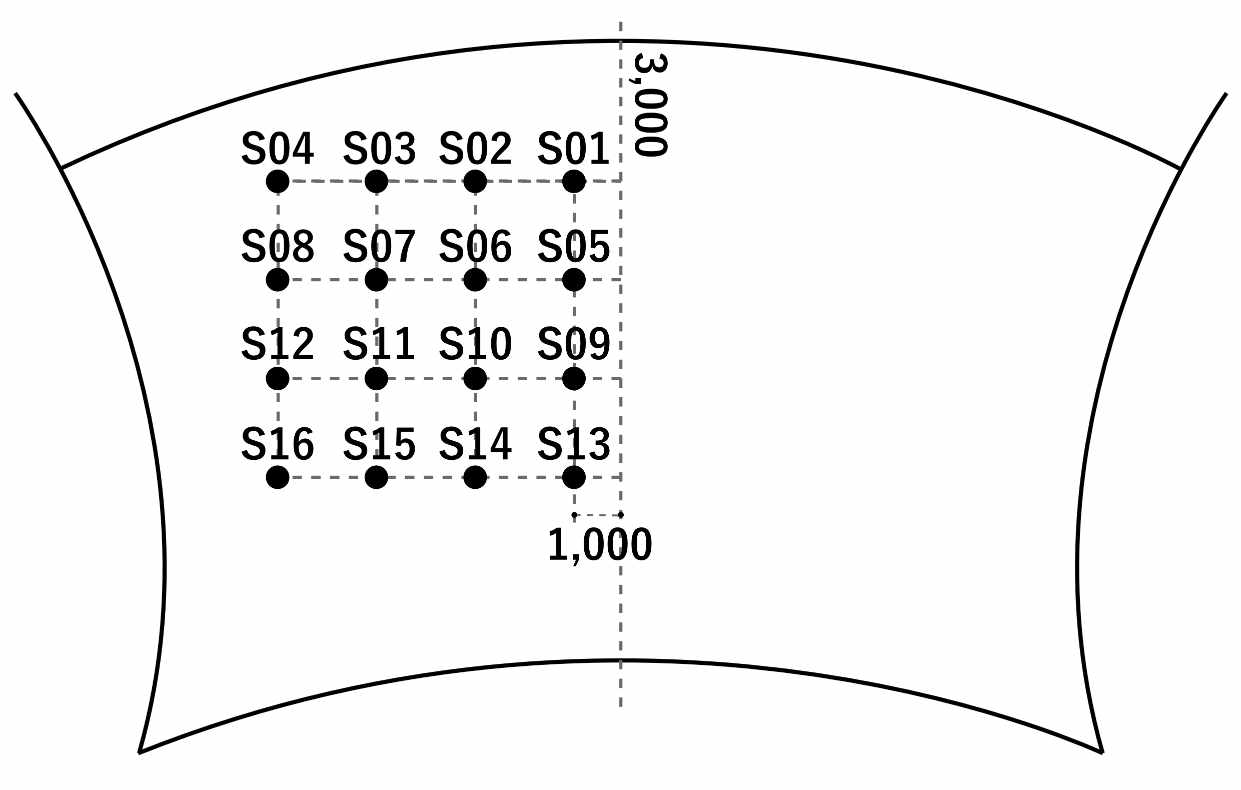
\includegraphics[width=.8\linewidth]{images/measuredHalls/resized/flat_g.jpg}
    \\ホールG 測定位置
  \end{minipage}%
  \begin{minipage}{.5\linewidth} % 右側の図
    \raggedleft
    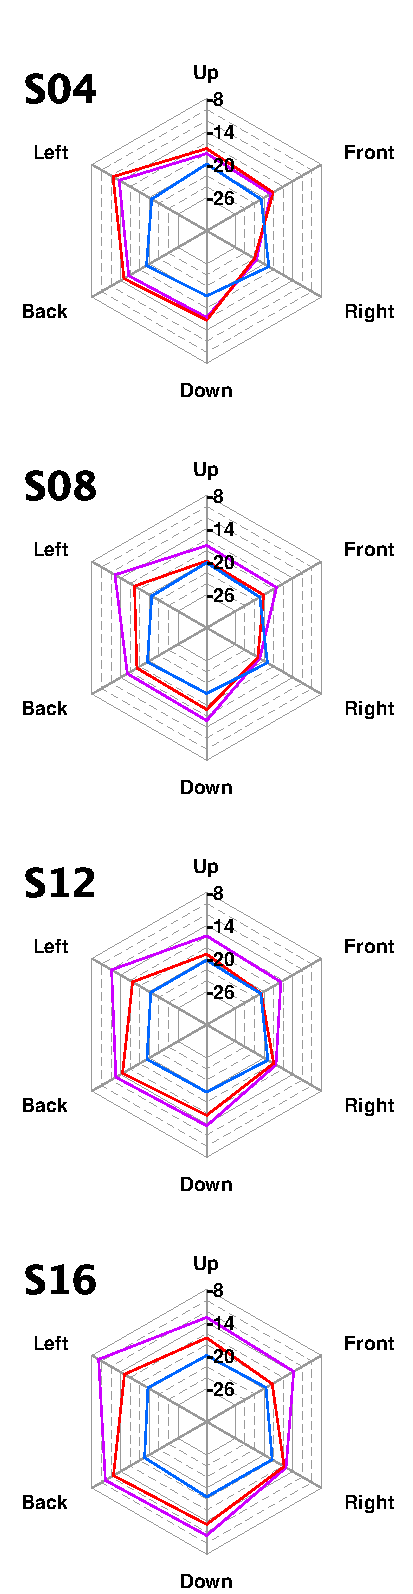
\includegraphics[scale=.77]{images/realHallDirSt/allPoint/reshaped/gLeftPage.pdf}
  \end{minipage}
\end{figure}

\newpage

\begin{figure}[H]
  \centering
  \includegraphics[scale=.77]{images/realHallDirSt/allPoint/reshaped/gRightPage.pdf}
  \caption{ホールG 方向別ST}
  \label{fig:ホールG 方向別ST}
\end{figure}

\clearpage

%=======================================================================
\subsection*{測定結果の考察}

前項にて、各ホールの全測定点における$\mathrm{ST_{Early,dir}}$、$\mathrm{ST_{Early,dir}}$および$10$~$\SI{100}{\ms}$での方向別反射音のエネルギーの評価値について、測定結果を示した。

さらに、$\mathrm{ST_{Early,dir}}$および$\mathrm{ST_{Early,dir}}$のホール間での傾向の違いについて、各ホールにおけるすべての測定点の平均値と最大値・最小値を図\ref{fig:方向別STEarlyのホール間での傾向の違い}および図\ref{fig:方向別STLateのホール間での傾向の違い}に示し、また$\mathrm{ST_{Early,dir}}$および$\mathrm{ST_{Early,dir}}$の測定位置による傾向の違いについて、各測定位置におけるすべてのホールでの平均値と最大値・最小値を図\ref{fig:各ホールの測定位置における方向別STEarlyの違い}および図\ref{fig:各ホールの測定位置における方向別STLateの違い}に示す。ただし、\ref{fig:各ホールの測定位置における方向別STEarlyの違い}および図\ref{fig:各ホールの測定位置における方向別STLateの違い}では、すべてのホールで測定を行った測定点であるS01、S02、S03、S05、S06、S07、S09、S10の結果について計算した。

\subsubsection{初期反射音に関する評価について}

$\mathrm{ST_{Early,dir}}$および$10$~$\SI{100}{\ms}$に到来する反射音については、全ホールに共通して方向別の偏差が見られ、方向ごとに強度が異なっていた。特に、すべての測定位置でFrontの値が相対的に低く、$\SI{100}{\ms}$までに到来する客席側からの反射音レベルが低くなっている傾向が見られた。

舞台中央側および前方側の測定点では$\mathrm{ST_{Early,dir}}$と$10$~$\SI{100}{\ms}$に到来する反射音の評価値はほぼ等しいのに対し、壁面との距離の近い舞台上手側および舞台奥付近の測定点では、特にLeftおよびBackの方向で$10$~$\SI{100}{\ms}$の評価値が$\mathrm{ST_{Early,dir}}$よりも顕著に大きくなる傾向が見られた。$\SI{100}{\ms}$以内に到来する反射に占める一次の反射音のエネルギーが大きく、これが評価区間に含まれるかどうかによって評価値が大きく変化していると考えられる。また、壁面の近傍における測定点ではこの一次の反射音の減衰も小さく、$10$~$\SI{20}{\ms}$に到来している成分のエネルギーが特に大きくなっていると考えられる。ごく短い遅れ時間で到来する反射音はカラレーションを引き起こす恐れがあり、$10$~$\SI{20}{\ms}$の間に到来する反射音もカラレーションを起こして心理印象を変化させる原因になりうるため、これらの点におけるエネルギー量に着目した指標での評価は心理印象とうまく対応しない可能性がある。


\subsubsection{後期反射音に関する評価について}
$\mathrm{ST_{Late,dir}}$については、方向別の差異が小さい傾向にあり、$100$~$\SI{1000}{\ms}$に到来する反射音は一様な強度になっていて、拡散してあらゆる方向から到来していると考えられる。また、同一のホール内での測定点毎の差も小さく、舞台上での位置依存性も小さいと推察される。一方で、ホール間での差異は大きい傾向にあり、ホールCおよびFは他のホールに比べて全体的に値が高くなっている。ホールCおよびFは残響時間も$\SI{2}{秒}$以上とホールA、B、D、Eに比べてかなり長くなっているが、同じく$\SI{2}{秒}$以上の長い残響時間を有すホールGにおける$\mathrm{ST_{Late,dir}}$は他のホールと同程度の水準である。ホールAからFがシューボックス型の形状をしているのに対し、ホールGはアリーナ型の形状であるため、ホールGでは残響時間の長さの割に演奏者に返る後期反射音が少なく、$\mathrm{ST_{Late,dir}}$がホールC、Fよりも小さくなっているのではないかと考えられる。
%=======================================================================

\newpage
\begin{figure}[H]
  \begin{minipage}[b]{.33\textwidth}
      \centering
      \includegraphics[width=1\linewidth]{images/realHallDirSt/early_hall_a_withLegend.png}
      \subcaption*{ホールA}
      \label{fig:ホールAにおけるSTEarly}
  \end{minipage}%
  \begin{minipage}[b]{.33\textwidth}
    \centering
    \includegraphics[width=1\linewidth]{images/realHallDirSt/early_hall_b_allpoints.png}
    \subcaption*{ホールB}
    \label{fig:ホールBにおけるSTEarly}
  \end{minipage}%
  \begin{minipage}[b]{.33\textwidth}
    \centering
    \includegraphics[width=1\linewidth]{images/realHallDirSt/early_hall_c_allpoints.png}
    \subcaption*{ホールC}
    \label{fig:ホールCにおけるSTEarly}
  \end{minipage}

  \begin{minipage}[b]{.33\textwidth}
    \centering
    \includegraphics[width=1\linewidth]{images/realHallDirSt/early_hall_d_allpoints.png}
    \subcaption*{ホールD}
    \label{fig:ホールDにおけるSTEarly}
  \end{minipage}%
  \begin{minipage}[b]{.33\textwidth}
    \centering
    \includegraphics[width=1\linewidth]{images/realHallDirSt/early_hall_e_allpoints.png}
    \subcaption*{ホールE}
    \label{fig:ホールEにおけるSTEarly}
  \end{minipage}%
  \begin{minipage}[b]{.33\textwidth}
    \centering
    \includegraphics[width=1\linewidth]{images/realHallDirSt/early_hall_f_allpoints.png}
    \subcaption*{ホールF}
    \label{fig:ホールFにおけるSTEarly}
  \end{minipage}

  \begin{minipage}[b]{.33\textwidth}
    \centering
    \includegraphics[width=1\linewidth]{images/realHallDirSt/early_hall_g_allpoints.png}
    \subcaption*{ホールG}
    \label{fig:ホールGにおけるSTEarly}
  \end{minipage}

\caption{各ホールにおける$\mathrm{ST_{Early,dir}}$}
\label{fig:各ホールにおけるSTEarly}
\end{figure}

%=======================================================================

\newpage
\begin{figure}[H]
  \begin{minipage}[b]{.33\textwidth}
      \centering
      \includegraphics[width=1\linewidth]{images/realHallDirSt/late_hall_a_withLegend.png}
      \subcaption*{ホールA}
      \label{fig:ホールAにおけるSTlate}
  \end{minipage}%
  \begin{minipage}[b]{.33\textwidth}
    \centering
    \includegraphics[width=1\linewidth]{images/realHallDirSt/late_hall_b_allpoints.png}
    \subcaption*{ホールB}
    \label{fig:ホールBにおけるSTlate}
  \end{minipage}%
  \begin{minipage}[b]{.33\textwidth}
    \centering
    \includegraphics[width=1\linewidth]{images/realHallDirSt/late_hall_c_allpoints.png}
    \subcaption*{ホールC}
    \label{fig:ホールCにおけるSTlate}
  \end{minipage}

  \begin{minipage}[b]{.33\textwidth}
    \centering
    \includegraphics[width=1\linewidth]{images/realHallDirSt/late_hall_d_allpoints.png}
    \subcaption*{ホールD}
    \label{fig:ホールDにおけるSTlate}
  \end{minipage}%
  \begin{minipage}[b]{.33\textwidth}
    \centering
    \includegraphics[width=1\linewidth]{images/realHallDirSt/late_hall_e_allpoints.png}
    \subcaption*{ホールE}
    \label{fig:ホールEにおけるSTlate}
  \end{minipage}%
  \begin{minipage}[b]{.33\textwidth}
    \centering
    \includegraphics[width=1\linewidth]{images/realHallDirSt/late_hall_f_allpoints.png}
    \subcaption*{ホールF}
    \label{fig:ホールFにおけるSTlate}
  \end{minipage}

  \begin{minipage}[b]{.33\textwidth}
    \centering
    \includegraphics[width=1\linewidth]{images/realHallDirSt/late_hall_g_allpoints.png}
    \subcaption*{ホールG}
    \label{fig:ホールGにおけるSTlate}
  \end{minipage}

\caption{各ホールにおける$\mathrm{ST_{Late,dir}}$}
\label{fig:各ホールにおけるSTLate}
\end{figure}

%=======================================================================

\newpage
\begin{figure}[H]
  \begin{minipage}[b]{.33\textwidth}
      \centering
      \includegraphics[width=1\linewidth]{images/realHallDirSt/early_S03_allhall.png}
      \subcaption*{測定点3}
      \label{fig:S03early}
  \end{minipage}%
  \begin{minipage}[b]{.33\textwidth}
    \centering
    \includegraphics[width=1\linewidth]{images/realHallDirSt/early_S02_allhall.png}
    \subcaption*{測定点2}
    \label{fig:S02early}
  \end{minipage}%
  \begin{minipage}[b]{.33\textwidth}
    \centering
    \includegraphics[width=1\linewidth]{images/realHallDirSt/early_S01_withLegend.png}
    \subcaption*{測定点1}
    \label{fig:S01early}
  \end{minipage}

  \begin{minipage}[b]{.33\textwidth}
    \centering
    \includegraphics[width=1\linewidth]{images/realHallDirSt/early_S07_allhall.png}
    \subcaption*{測定点7}
    \label{fig:S07early}
  \end{minipage}%
  \begin{minipage}[b]{.33\textwidth}
    \centering
    \includegraphics[width=1\linewidth]{images/realHallDirSt/early_S06_allhall.png}
    \subcaption*{測定点6}
    \label{fig:S06early}
  \end{minipage}%
  \begin{minipage}[b]{.33\textwidth}
    \centering
    \includegraphics[width=1\linewidth]{images/realHallDirSt/early_S05_allhall.png}
    \subcaption*{測定点5}
    \label{fig:S04early}
  \end{minipage}

  \begin{minipage}[b]{.33\textwidth}
    \hspace{1 \linewidth}
  \end{minipage}%
  \begin{minipage}[b]{.33\textwidth}
    \centering
    \includegraphics[width=1\linewidth]{images/realHallDirSt/early_S10_allhall.png}
    \subcaption*{測定点10}
    \label{fig:S10early}
  \end{minipage}%
  \begin{minipage}[b]{.33\textwidth}
    \centering
    \includegraphics[width=1\linewidth]{images/realHallDirSt/early_S09_allhall.png}
    \subcaption*{測定点9}
    \label{fig:S09early}
  \end{minipage}

\caption{各測定点における$\mathrm{ST_{Early,dir}}$(全ホール)}
\label{fig:各測定点におけるSTEarly}
\end{figure}

%=======================================================================

\newpage
\begin{figure}[H]
  \begin{minipage}[b]{.33\textwidth}
      \centering
      \includegraphics[width=1\linewidth]{images/realHallDirSt/late_S03_allhall.png}
      \subcaption*{測定点3}
      \label{fig:S03late}
  \end{minipage}%
  \begin{minipage}[b]{.33\textwidth}
    \centering
    \includegraphics[width=1\linewidth]{images/realHallDirSt/late_S02_allhall.png}
    \subcaption*{測定点2}
    \label{fig:S02late}
  \end{minipage}%
  \begin{minipage}[b]{.33\textwidth}
    \centering
    \includegraphics[width=1\linewidth]{images/realHallDirSt/late_S01_withLegend.png}
    \subcaption*{測定点1}
    \label{fig:S01late}
  \end{minipage}

  \begin{minipage}[b]{.33\textwidth}
    \centering
    \includegraphics[width=1\linewidth]{images/realHallDirSt/late_S07_allhall.png}
    \subcaption*{測定点7}
    \label{fig:S07late}
  \end{minipage}%
  \begin{minipage}[b]{.33\textwidth}
    \centering
    \includegraphics[width=1\linewidth]{images/realHallDirSt/late_S06_allhall.png}
    \subcaption*{測定点6}
    \label{fig:S06late}
  \end{minipage}%
  \begin{minipage}[b]{.33\textwidth}
    \centering
    \includegraphics[width=1\linewidth]{images/realHallDirSt/late_S05_allhall.png}
    \subcaption*{測定点5}
    \label{fig:S04late}
  \end{minipage}

  \begin{minipage}[b]{.33\textwidth}
    \hspace{1 \linewidth}
  \end{minipage}%
  \begin{minipage}[b]{.33\textwidth}
    \centering
    \includegraphics[width=1\linewidth]{images/realHallDirSt/late_S10_allhall.png}
    \subcaption*{測定点10}
    \label{fig:S10late}
  \end{minipage}%
  \begin{minipage}[b]{.33\textwidth}
    \centering
    \includegraphics[width=1\linewidth]{images/realHallDirSt/late_S09_allhall.png}
    \subcaption*{測定点9}
    \label{fig:S09late}
  \end{minipage}

\caption{各測定点における$\mathrm{ST_{Late,dir}}$(全ホール)}
\label{fig:各測定点におけるSTLate}
\end{figure}


%=======================================================================

\newpage
\section{生成音場の目標値の設定}
方向特性の評価を行う演奏実験を行うために生成する音場について、実際のコンサートホールのステージ上の音場に近づけることを目指すため、前節までに示したコンサートホールのステージにおける実測結果に基づいて設定する。

%=======================================================================

\newpage
\subsection*{実験室における音場の可変幅の確認}
実験室に響きを付加するにあたり、目標とした音場が実験室で実現可能な響きの幅、すなわち最小の響きの条件と最大の響きの範囲に収まることを確認する必要がある。

AFCは響きを増幅するシステムであるため、実験室で実現可能な最小の響きは、AFCをオフにしたときの響きとなる。AFCをオフししたときの$\mathrm{ST_{Early,dir}}$、$\mathrm{ST_{Late,dir}}$を表\ref{table:響き小の方向別ST}に示す。

\begin{table}[H]
  \centering
  \caption{AFCをオフにしたときの$\mathrm{ST_{Early,dir}}$、$\mathrm{ST_{Late,dir}}$}
  \label{table:響き小の方向別ST}
  \begin{tabular}{c|cccccc} \hline \hline
    \begin{tabular}{c}
    
    \end{tabular}&
    \begin{tabular}{c}
      Front
    \end{tabular}&
    \begin{tabular}{c}
      Back
    \end{tabular}&
    \begin{tabular}{c}
      Left
    \end{tabular}&
    \begin{tabular}{c}
      Right
    \end{tabular}&
    \begin{tabular}{c}
      Up
    \end{tabular}&
    \begin{tabular}{c}
      Down
    \end{tabular} \\ \hline
    $\mathrm{ST_{Early,dir}}$ (dB) & -24.2 & -25.5 & -24.2 & -25.9 &-25.9 & -23.3 \\
    $\mathrm{ST_{Late,dir}}$ (dB) & -65.5 & -66.7 & -67.0 &-65.6 & -66.6 & -64.2 \\ \hline \hline
  \end{tabular}
\end{table}

響きを増やすことに関してはある程度自由度を持って調整することができるが、AFCでつける響きを大きくしていく、つまり再生音の音量を上げていくと、ある音量を超えたときに不自然な音色の変化(カラレーション)が発生し始める。カラレーションが起こり始める音量の条件はイコライザの設定等様々な要素によって変化するため最大の響きを厳密に調べることは困難である。
    
実験室での可変幅の大まかな検討のため、イコライザによる周波数特性の手動調整を行わずに仮の設定でAFCをオンにし、カラレーションの生じ始めを聴感的に確認し、その直前の音量の設定における$\mathrm{ST_{Early,dir}}$および$\mathrm{ST_{Late,dir}}$を測定した。その結果を表\ref{table:響き大の方向別ST}に示す。

\begin{table}[H]
  \centering
  \caption{AFC仮調整時の$\mathrm{ST_{Early,dir}}$、$\mathrm{ST_{Late,dir}}$}
  \label{table:響き大の方向別ST}
  \begin{tabular}{c|cccccc} \hline \hline
    \begin{tabular}{c}
    
    \end{tabular}&
    \begin{tabular}{c}
      Front
    \end{tabular}&
    \begin{tabular}{c}
      Back
    \end{tabular}&
    \begin{tabular}{c}
      Left
    \end{tabular}&
    \begin{tabular}{c}
      Right
    \end{tabular}&
    \begin{tabular}{c}
      Up
    \end{tabular}&
    \begin{tabular}{c}
      Down
    \end{tabular} \\ \hline
    $\mathrm{ST_{Early,dir}}$ (dB) & -16.4 & -18.0 & -16.7 & -17.3 & -19.9 & -16.1\\
    $\mathrm{ST_{Late,dir}}$ (dB) & -15.8 & -15.9 & -16.0 & -15.8 & -19.2 & -15.0\\ \hline \hline
  \end{tabular}
\end{table}

    

これらの結果とコンサートホールでの実測値から、実験室における$\mathrm{ST_{Early,dir}}$と$\mathrm{ST_{Late,dir}}$はコンサートホールでの実測値と同程度の値を十分取ることができると考えられ、詳細な設定により所望の音場を実現しうることが期待できる。

%=======================================================================


% 参考文献
% 参考文献の箇所にインプットしてください。

% 分割ファイル内でのみ,bibliographyを読み込みます。

\expandafter\ifx\csname ifdraft\endcsname\relax

  % bibliographyを展開する

  \bibliographystyle{junsrt}
  \bibliography{ref.bib}% 同じディレクトリ内のbibファイルのみを参照可能

\fi

\end{document}

%=======================================================================
\cleardoublepage
\documentclass[11pt,a4j]{jreport}

\usepackage{comment}
\usepackage{float}
\usepackage{color}
\usepackage{multicol}
\usepackage{multirow}
\usepackage[dvipdfmx]{pict2e}
\usepackage{wrapfig}
\usepackage{graphicx}
\usepackage{bm}
\usepackage{url}
\usepackage{underscore}
\usepackage{colortbl}
\usepackage{tabularx}
\usepackage{fancyhdr}
\usepackage{ulem}
\usepackage{cite}
\usepackage{amsmath,amssymb,amsfonts}
\usepackage{algorithmic}
\usepackage{textcomp}
\usepackage{xcolor}
\usepackage[ipaex]{pxchfon}
\usepackage{pdfpages}
\usepackage{subcaption}
\usepackage{array}
\usepackage{adjustbox}
\usepackage{lipsum}

\usepackage[number-unit-product=~]{siunitx}

\usepackage[top=30truemm,bottom=30truemm,left=25truemm,right=25truemm]{geometry}

\renewcommand{\arraystretch}{1.2}

\begin{document}

\chapter{実験音場の生成}

第2章にて、コンサートホールのステージ上における反射音の到来方向を定量化する指標として$\mathrm{ST_{Early,dir}}$および$\mathrm{ST_{Late,dir}}$を定義し、その実測値をもとに演奏実験に用いるために生成する音場の目標値を設定した。

本章では、音場生成システムAFCを用いた実験音場の生成に関して述べる。まず、本研究で音場生成に用いるシステムである音場支援システムAFCとそれを導入した実験室(半無響室)について紹介する。続いて、生成する音場での方向別STおよび周波数特性の調整を含む残響時間とSTの調整方法について、音場の生成における考え方とそれに基づく具体的な調整値について説明する。最後に、コンサートホールを模して生成した音場を基準音場として、基準音場の音響特性と、基準音場から方向特性を変化させた音場の音響特性を測定した結果結果を示す。


\section{音場支援システムAFCについて}

\subsection*{音場支援システムの概要}
第1章4節でも触れたように、音場支援システム(Active Field Control Enhance、AFC)は、一つの空間において多様な演目を最適な響きの中で行いたいというモチベーションから開発されたシステムであり、最新の電気音響・信号処理技術を用いて、室内の響きや空間の拡がり・音量感などの聴感印象を自然に変化させることができる\cite{AFCの概要}。音源自体に人工的なリバーブを付加して異なる音の印象を作り出す手法とは異なり、楽器や歌声の自然な聴こえ方を保ちながら、その空間に拡がる音の残響感や音量感をコントロールし、用途に適した音響空間を提供できる点にその特徴がある。

マイクロフォンとスピーカーを配置して音場を生成するシステムにおける信号処理の方式は、マイクで収音した音をスピーカーから再生し、スピーカーからの再生音に空間固有の響きが加わった音を再びマイクで収音する音響的フィードバックを利用する室内音場制御方式と、収音した音に様々な実測インパルス応答のデータを畳み込むことで任意の音場を再現する音場合成方式の二つの方式に大別され、AFCではこれら二つの方式を兼ね備えたハイブリッドなシステムとして構成されている\cite{AFCEnhance}。

%=======================================================================
\newpage
\subsection*{音場支援システムの仕組み}
響きの聴覚印象には初期反射音と残響音(後期反射音)がそれぞれ異なる影響を与えていると考えられ、AFCにおける音響信号の処理系統も、初期反射音制御部と後期反射音制御部に大きく分かれてそれぞれの反射音成分をある程度独立に制御している。この概略図を図\ref{fig:AFCにおける初期反射音と後期反射音の制御の概略図}に示す。

どちらの制御部においても、マイクロホンで収音した音に対してインパルス応答の畳み込みによる響きの付加を行ってからスピーカーでその信号を再生し、響きを増幅させる点は共通している。初期反射音制御部では演奏者の付近に設置した指向性マイクによって主に直接音と舞台上からの初期反射音を収音して初期反射音成分に相当する響きをスピーカーから再生させるのに対し、後期反射音制御部では演奏者から遠方に付置した全指向性マイクによって主に空間の残響音とスピーカーから再生される音響フィードバック成分を収音して後期反射音に相当する響きをスピーカーから再生させている。

初期・後期どちらの制御部でも室内音場制御方式と音場合成方式を組み合わせた制御方式となっており、AFC内部での信号処理の流れは次の通りである。まず、室内に配置された各マイクに収音された信号がbusと呼ばれる信号処理系に割り振られる。続いて、busに割り振られた音響信号に対して「FIRフィルタの重畳」「遅れ時間の付与」「音量の増減」「イコライザによる周波数特性の変化」が組み合わせて適用される。そして、busによって処理された音響信号は室内に配置されたスピーカーに割り振られて出力される。このbusごとの信号処理の概要を図\ref{fig:busごとの信号処理の概要}に示す。

AFCではスピーカーから再生された音がマイクへ戻る音響的フィードバックを利用するため、生成する響きを大きくしようとするとループゲインが増大してハウリングが発生しやすくなる恐れがあることが重要な技術的課題となっている。そこでAFCでは、マイクからbusへのルーティングを時変的に切り替えることによってハウリングの発生を抑制する処理であるヤマハ独自の特許技術EMR(Electronic Microphone Rotator)\cite{清水1996EMR}が使用されている。AFCにおける信号処理系は4つのbusを1組の「System」として管理され、EMRは主に後期反射音の制御用に割り当てられたSystemにおいて適用される。このSystemごとの信号処理の概要を図\ref{fig:Systemによる信号処理の概要}に示す。

\vspace{\stretch{1}}

\begin{figure}[H]
  \centering
  \includegraphics[width=0.8\linewidth]{images/AFCsystemOverView.png}
  \caption{AFCにおける初期反射音と後期反射音の制御の概略図}
  \label{fig:AFCにおける初期反射音と後期反射音の制御の概略図}
\end{figure}

\vspace{\stretch{1}}
%=======================================================================
\newpage

\vspace*{\stretch{1}}
\begin{figure}[H]
  \centering
  \includegraphics[width=0.9\linewidth]{images/AFCbusProcessing.png}
  \caption{busごとの信号処理の概要}
  \label{fig:busごとの信号処理の概要}
\end{figure}

\vspace*{\stretch{1}}

\begin{figure}[H]
  \centering
  \includegraphics[width=0.9\linewidth]{images/AFCsystemProcessing.png}
  \caption{Systemによる信号処理の概要}
  \label{fig:Systemによる信号処理の概要}
\end{figure}

\vspace*{\stretch{1}}
%=======================================================================

\newpage
\subsection*{実験室におけるAFCのシステム機器配置}
もともとの響きの小さい室でAFCを用いることにより、大きな制御幅を得て自由度の高い音場の生成を行えることが期待できるため、本実験では半無響室にAFCを導入して用いることとした。導入したAFCシステムを構成する音響機材は4つのカージオイドマイク、4つの無指向性マイク、および20個のスピーカーであり、実験室の内部の様子を図\ref{fig:実験室の内部の様子}に、音響機材の配置を図\ref{fig:AFCのシステム機器配置}に示す。

また、生成する音場の評価を行うための音響測定は実験室の中央で行うものとし、音響測定時の測定機器の配置を図\ref{fig:音響測定機器の配置}に、そのときの様子を図\ref{fig:音響測定時の様子}示す。なお、紙面の上方を実験室の前方として実験室内における方向を定義した。

\vspace{\stretch{1}}
\begin{figure}[H]
  \centering
  \includegraphics[width=0.6\linewidth]{images/twoPiRoom/twoPiRoomPhoto.png}
  \caption{実験室の内部の様子}
  \label{fig:実験室の内部の様子}
\end{figure}

\begin{figure}[H]
  \begin{minipage}[b]{0.5\linewidth}
    \centering
    \includegraphics[width=.9\linewidth]{images/twoPiRoom/measureSetting.png}
    \caption{音響測定機器の配置}
    \label{fig:音響測定機器の配置}
  \end{minipage}%
  \begin{minipage}[b]{0.5\linewidth}
    \centering
    \includegraphics[width=.9\linewidth]{images/twoPiRoom/measureSettingPhotoResized.jpg}
    \caption{音響測定時の様子}
    \label{fig:音響測定時の様子}
  \end{minipage}
\end{figure}

\vspace{\stretch{1}}
%=======================================================================

\newpage
\vspace*{\stretch{1}}
\begin{figure}[H]
  \begin{minipage}[b]{1\linewidth}
    \centering
    \includegraphics[width=.6\linewidth]{images/twoPiRoom/afcEquipArrayVertical.png}
    \subcaption{断面図}
    \label{fig:AFC機器配置断面図}
  \end{minipage}

  \begin{minipage}[b]{0.5\linewidth}
    \centering
    \includegraphics[width=.9\linewidth]{images/twoPiRoom/afcEquipArrayMic.png}
    \subcaption{マイクロホン配置}
    \label{fig:マイクロホン配置}
  \end{minipage}%
  \begin{minipage}[b]{0.5\linewidth}
    \centering
    \includegraphics[width=.9\linewidth]{images/twoPiRoom/afcEquipArraySp3.png}
    \subcaption{スピーカー配置 三層目}
    \label{fig:スピーカー配置 三層目}
    \vfill
  \end{minipage}

  \begin{minipage}[b]{0.5\linewidth}
    \centering
    \includegraphics[width=.9\linewidth]{images/twoPiRoom/afcEquipArraySp2.png}
    \subcaption{スピーカー配置 二層目}
    \label{fig:スピーカー配置 二層目}
  \end{minipage}%
  \begin{minipage}[b]{0.5\linewidth}
    \centering
    \includegraphics[width=.9\linewidth]{images/twoPiRoom/afcEquipArraySp1.png}
    \subcaption{スピーカー配置 一層目}
    \label{fig:スピーカー配置 一層目}
    \vfill
  \end{minipage}

  \caption{AFCのシステム機器配置}
  \label{fig:AFCのシステム機器配置}
\end{figure}
\vspace{\stretch{1}}

%=======================================================================
%\newpage
\section{音場生成の準備}
前節にてAFCシステムの仕組みと本研究で用いる実験室およびシステム機器構成について紹介した。本節ではAFCで音場生成を行う前の準備事項に関して、まず実験室に配置したマイクとスピーカーのルーティングについて、続いて調整で用いるFIRフィルタについて、最後に実験室における響きの制御幅について述べる。

\subsection*{マイクとスピーカーのルーティング}
2章4節にて設定した目標値を踏まえて、まず音場生成時のマイクとスピーカーのルーティングを決定する。前節で示したように、AFCのマイク入力はbusと呼ばれる信号処理系に割り当てられ、さらに4つのbusを一つのSystemとして取り扱う。本研究では、5つのSystemを作成して音場の生成を行った。

System1は、大まかな初期反射音成分の付加のため、入力系としてカージオイドマイクであるMic.1〜4の信号を用い、出力系として後方側からの再生音がやや多くなるように全方向のスピーカーを割り当てた。

System2は、水平面内からの全体的な後期反射音を満遍なく付加するため、マイクの入力とbusのルーティングを切り替える処理であるEMRをオンにした上で、入力系として全指向性マイクであるMic.5〜8の信号を用い、出力系として実験室の対角線上に配置した8つのスピーカーを割り当てた。

System3は、System2のみでは不足する上方からの後期反射音を増強して供給するため、入力系として全指向性マイクであるMic.5〜8の信号を用い、出力系として実験室の天井に設置した4つのスピーカーを割り当てた。

System4は、System1ではエネルギーの量が不足する後方からの初期反射音を増強しつつ、System1で小さくなるように調整する前方から初期反射音の供給量を細かく調整できるよう、出力系として実験室の後方に設置した3つのスピーカーと、前方に設置した1つのスピーカーを割り当てた。入力系としては、カージオイドマイクであるMic.1〜4を用いた場合にカラレーションが発生したため、全指向性マイクであるMic.5〜8の信号を用いた。

System5は、後期反射音の制御系だが、EMRの利用による後期反射音の方向特性の時変的な変化を是正して安定させるため、EMRの利用によるルーティングの切り替えは行わずに、全指向性マイクであるMic.5〜8の信号を用い、出力系として実験室の前後左右方向に設置した4つのスピーカーを割り当てた。

初期反射音および後期反射音ともに、床からの反射音供給によって、上方よりも下方からの寄与が大きくなる傾向が見られたため、System4およびSystem5では、前後左右方向の反射音供給を行うスピーカーとして、床面に近い1層目ではなく、床面から離れた2層目のスピーカーを用いた。

これらのルーティングを表\ref{tab:マイクとスピーカーのルーティング}に示す。

\newpage
\vspace*{\stretch{1}}
\begin{table}[H]
  \centering
  \caption{マイクとスピーカーのルーティング}
  \label{tab:マイクとスピーカーのルーティング}
  \includegraphics[width=1\linewidth]{images/experimentField/micSpRooting.pdf}
\end{table}
\vspace*{\stretch{1}}

%=======================================================================
\newpage
\subsection*{重畳に用いるFIRフィルタ}
響きの可変幅を十分に確保できるよう、重畳するFIRフィルタには図\ref{fig:FIRフィルタを測定したコンサートホール}に示す2000席程度の豊かな響きを持つコンサートホールにて実測したインパルス応答を用いた。初期反射音制御部には舞台付近で測定したインパルス応答を、後期反射音制御部には舞台から遠方にて測定したインパルス応答を用いた。それぞれについて、ともに異なる4点で測定したインパルス応答を用いており、これは完全に同じインパルス応答を用いることによってAFCシステム内のループごとの周波数特性が近くなることでカラレーションに対する安定性が低下するのを防ぐことを目的としている。重畳に用いたインパルス応答の時間波形を図\ref{fig:初期反射音の重畳に用いたFIRフィルタ}および図\ref{fig:後期反射音の重畳に用いたフィルタ}に示す。

\lipsum[1-2]

\vspace{\stretch{1}}
\begin{figure}[H]
  \centering
  \includegraphics[width=.5\linewidth]{images/convolutedIrHall.jpg}
  \caption{FIRフィルタを測定したコンサートホール}
  \label{fig:FIRフィルタを測定したコンサートホール}
\end{figure}
\vspace{\stretch{1}}

%=======================================================================
\newpage

\vspace*{\stretch{1}}
\begin{figure}[H]
  \begin{minipage}[b]{.5\linewidth}
    \centering
    \includegraphics[width=.8\linewidth]{images/convolutedIr/ER1.png}
    \subcaption*{FIRフィルタ 1}
  \end{minipage}%
  \begin{minipage}[b]{.5\linewidth}
    \centering
    \includegraphics[width=.8\linewidth]{images/convolutedIr/ER2.png}
    \subcaption*{FIRフィルタ 2}
  \end{minipage}

  \begin{minipage}[b]{.5\linewidth}
    \centering
    \includegraphics[width=.8\linewidth]{images/convolutedIr/ER3.png}
    \subcaption*{FIRフィルタ 3}
  \end{minipage}%
  \begin{minipage}[b]{.5\linewidth}
    \centering
    \includegraphics[width=.8\linewidth]{images/convolutedIr/ER4.png}
    \subcaption*{FIRフィルタ 4}
  \end{minipage}

  \centering
  \caption{初期反射音の重畳に用いたFIRフィルタ}
  \label{fig:初期反射音の重畳に用いたFIRフィルタ}
\end{figure}

\begin{figure}[H]
  \begin{minipage}[b]{.5\linewidth}
    \centering
    \includegraphics[width=.8\linewidth]{images/convolutedIr/REV1.png}
    \subcaption*{FIRフィルタ 1}
  \end{minipage}%
  \begin{minipage}[b]{.5\linewidth}
    \centering
    \includegraphics[width=.8\linewidth]{images/convolutedIr/REV2.png}
    \subcaption*{FIRフィルタ 2}
  \end{minipage}

  \begin{minipage}[b]{.5\linewidth}
    \centering
    \includegraphics[width=.8\linewidth]{images/convolutedIr/REV3.png}
    \subcaption*{FIRフィルタ 3}
  \end{minipage}%
  \begin{minipage}[b]{.5\linewidth}
    \centering
    \includegraphics[width=.8\linewidth]{images/convolutedIr/REV4.png}
    \subcaption*{FIRフィルタ 4}
  \end{minipage}

  \centering
  \caption{後期反射音の重畳に用いたFIRフィルタ}
  \label{fig:後期反射音の重畳に用いたフィルタ}
\end{figure}
\vspace{\stretch{1}}
%=======================================================================

\newpage
\subsection*{AFCの音場生成における制御幅}
実験室に響きを付加するにあたり、目標とした音場が実験室で実現可能な響きの幅、すなわち最小の響きの条件と最大の響きの範囲に収まることを確認する必要がある。

AFCは響きを増幅するシステムであるため、実験室で実現可能な最小の響きは、AFCをオフにしたときの響きとなる。AFCをオフししたときの$\mathrm{ST_{Early,dir}}$、$\mathrm{ST_{Late,dir}}$を表\ref{table:響き小の方向別ST}に示す。

この結果、AFCをオフにしたときの$\mathrm{ST_{Late,dir}}$は非常に小さく、この評価区間では音がほぼ完全に吸音されており、後期反射音についてはシステムで付加する成分によってほぼ完全に決定されると考えられる。一方で、$\mathrm{ST_{Early,dir}}$は$\SI{-25}{\dB}$前後と、$\mathrm{ST_{Late,dir}}$に比べて大きな値となっていた。これは半無響室に配置した吸音材に吸音され切らなかった低次の反射音がわずかに$100$〜$\SI{100}{\ms}$の間に残っているためと考えられる。特にFront方向では図\ref{fig:生成音場の目標値}に示した基準音場の生成目標値との差が約$\SI{3}{\dB}$に迫っており、慎重な調整が必要となる。

響きを増やすことに関してはある程度自由度を持って調整することができるが、AFCでつける響きを大きくしていく、つまり再生音の音量を上げていくと、ある音量を超えたときに不自然な音色の変化(カラレーション)が発生し始める。カラレーションが起こり始める音量の条件はイコライザの設定による周波数特性の変化をはじめとする様々な要素によって変化し、最大の響きの条件を厳密に調べることはできないが、イコライザによる周波数特性の補正を行わずに、その分のゲインの稼得を残す安全側にて響きの可変幅を大まかに検討する。周波数特性の手動調整を行わずに仮の設定でAFCをオンにして、カラレーションの生じ始めを聴感的に確認し、その直前の音量の設定における$\mathrm{ST_{Early,dir}}$および$\mathrm{ST_{Late,dir}}$を測定した。その結果を表\ref{table:響き大の方向別ST}に示す。

これらの結果から、実験室における$\mathrm{ST_{Early,dir}}$と$\mathrm{ST_{Late,dir}}$はコンサートホールでの実測値と同程度の値を十分取ることができると考えられ、詳細な設定により所望の音場を実現しうることが期待できる。

\vspace{\stretch{1}}
\begin{table}[H]
  \centering
  \caption{AFCをオフにしたときの$\mathrm{ST_{Early,dir}}$、$\mathrm{ST_{Late,dir}}$}
  \label{table:響き小の方向別ST}
  \begin{tabular}{c|cccccc} \hline \hline
    \begin{tabular}{c}
    
    \end{tabular}&
    \begin{tabular}{c}
      Front
    \end{tabular}&
    \begin{tabular}{c}
      Back
    \end{tabular}&
    \begin{tabular}{c}
      Left
    \end{tabular}&
    \begin{tabular}{c}
      Right
    \end{tabular}&
    \begin{tabular}{c}
      Up
    \end{tabular}&
    \begin{tabular}{c}
      Down
    \end{tabular} \\ \hline
    $\mathrm{ST_{Early,dir}}$ (dB) & -24.2 & -25.5 & -24.2 & -25.9 &-25.9 & -23.3 \\
    $\mathrm{ST_{Late,dir}}$ (dB) & -65.5 & -66.7 & -67.0 &-65.6 & -66.6 & -64.2 \\ \hline \hline
  \end{tabular}
\end{table}

\begin{table}[H]
  \centering
  \caption{AFC仮調整時の$\mathrm{ST_{Early,dir}}$、$\mathrm{ST_{Late,dir}}$}
  \label{table:響き大の方向別ST}
  \begin{tabular}{c|cccccc} \hline \hline
    \begin{tabular}{c}
    
    \end{tabular}&
    \begin{tabular}{c}
      Front
    \end{tabular}&
    \begin{tabular}{c}
      Back
    \end{tabular}&
    \begin{tabular}{c}
      Left
    \end{tabular}&
    \begin{tabular}{c}
      Right
    \end{tabular}&
    \begin{tabular}{c}
      Up
    \end{tabular}&
    \begin{tabular}{c}
      Down
    \end{tabular} \\ \hline
    $\mathrm{ST_{Early,dir}}$ (dB) & -16.4 & -18.0 & -16.7 & -17.3 & -19.9 & -16.1\\
    $\mathrm{ST_{Late,dir}}$ (dB) & -15.8 & -15.9 & -16.0 & -15.8 & -19.2 & -15.0\\ \hline \hline
  \end{tabular}
\end{table}

\vspace{\stretch{1}}
%=======================================================================
\newpage
    

%=======================================================================

  \section{生成音場の調整方法}
    
    \subsection{方向別STの調整方法}
 
    $\mathrm{ST_{Early,dir}}$および$\mathrm{ST_{Late,dir}}$を目標値に近づけて制御するためには、初期反射音と
    後期反射音の成分をある程度独立に制御することが必要となる。初期反射音制御部のために付加したエネルギーが後期反射音の
    評価区間に漏れ出す量を少なくするため、初期反射音制御部では重畳するFIRフィルタにフェードアウトを設定することにより
    信号長を$\SI{120}{ms}$に限定した。
    
    また、後期反射音制御部では、反射音の付加に長い遅れ時間を加えることで$\mathrm{ST_{Early,dir}}$の評価区間に入るエネルギーを
    減らすことができるが、遅れ時間が大きすぎるとエコー障害が生じる恐れがある。本研究では、$\SI{45}{ms}$の遅れ時間を
    付け加えることにより、聴感的な自然さを保ちつつ$\mathrm{ST_{Early,dir}}$への影響を低減した。

    \subsection{その他の音響特性の調整方法}
      \subsubsection{残響時間の調整}
      本実験で用いた実験室における音響測定では、部屋の広さによる制約により、直接音の減衰が大きいため残響時間の評価として
      よく用いられる $\mathrm{T_{20}}$ または $\mathrm{T_{30}}$ を適切に測定することができない。
      そこで本研究では、$\mathrm{ST}$の測定条件によるインパルス応答の測定結果からエネルギーの減衰曲線を描き、
      $\SI{-15}{dB}$から$\SI{-45}{dB}$までの減衰曲線の傾きを読むことにより残響時間を求めた。
      生成した音場の残響時間は通常よくあるコンサートホールでの残響時間よりもかなり長くなる傾向があったため、
      後期反射音制御部で重畳するFIRフィルタにフェードアウトを設定することで残響時間を短くし、$\SI{1.8}{秒}$程度
      の自然な長さになるよう調整した。
      
      \subsubsection{周波数特性の調整}
      オクターブバンドごとのSTおよび残響時間の値が極端にばらつくことを防ぐため、測定とAFCシステム内部の
      イコライザの調整を繰り返して周波数特性を調整した。

%=====================================================================================

\section{生成した音場の特性}

  \subsection{基準音場}
  コンサートホールのステージを模して生成した基準音場の方向別STを図\ref{fig:基準音場の方向別ST}に示す。
  各方向での目標値からの差はすべて$\SI{1}{dB}$未満であり、およそ目標値の通りの方向別STを実現することが
  できた。
  
  残響時間およびSTを図\ref{fig:基準音場の残響時間とST}に示す。残響時間および$\mathrm{ST_{Late,dir}}$は
  すべてのオクターブバンドでほぼフラットな周波数特性となった。$\mathrm{ST_{Early,dir}}$は室自体の持つ特性
  が影響していると考えられ、完全な制御はできていないが、平均値からの偏差はすべてのオクターブバンドで$\SI{1}{dB}$
  程度に収めることができた。
  
  減衰曲線を図\ref{fig:基準音場の減衰曲線}に示す。AFCで生成した音場では、エネルギーの付加によって特に響きの
  後期反射音側で減衰曲線が盛り上がる場合があるが、今回生成した音場ではこのような現象は見られず、実際の空間と
  同様の直線的な減衰が確認できた。

  \begin{figure}[H]
    \begin{minipage}
      [b]{.5\linewidth}
      \centering
      \includegraphics[width=1\linewidth]{images/experimentField/withLegend/baseEarlyOnTarget4.png}
      \subcaption*{$\mathrm{ST_{Early,dir}}$}
    \end{minipage}%
    \begin{minipage}
      [b]{.5\linewidth}
      \centering
      \includegraphics[width=1\linewidth]{images/experimentField/withLegend/baseLateOnTarget4.png}
      \subcaption*{$\mathrm{ST_{Late,dir}}$}
      \end{minipage}
    \caption{基準音場の方向別ST}
    \label{fig:基準音場の方向別ST}
  \end{figure}

  \begin{figure}[H]
    \centering
    \includegraphics[width=.8\linewidth]{images/fieldO_stRt.png}
    \caption{基準音場の残響時間とST}
    \label{fig:基準音場の残響時間とST}
  \end{figure}

  \begin{figure}[H]
    \centering
    \includegraphics[width=.8\linewidth]{images/fieldO_EnergyDecayCurve.png}
    \caption{基準音場の減衰曲線}
    \label{fig:基準音場の減衰曲線}
  \end{figure}

  %=====================================================================================

  \subsection{方向の偏りをつけた音場}
  基準音場に対して、初期反射音・後期反射音のそれぞれについて、前方からの反射を強めた音場と後方からの反射を
  強めた音場を生成した。初期反射音の前方を強めた音場を音場A、初期反射音の後方を強めた音場を音場B、後期反射音の
  前方を強めた音場を音場C、後期反射音の後方を強めた音場を音場Dとする。生成した音場の方向別STを
  図\ref{fig:音場Aの方向別ST}から図\ref{fig:音場Dの方向別ST}に示す。

  \begin{figure}[H]
    \begin{minipage}[b]{.5\linewidth}
        \centering
        \includegraphics[width=1\linewidth]{images/experimentField/withLegend/expAEarly.png}
        \subcaption*{$\mathrm{ST_{Early,dir}}$\\前方強め}
    \end{minipage}%
    \begin{minipage}[b]{.5\linewidth}
        \centering
        \includegraphics[width=1\linewidth]{images/experimentField/withLegend/expALate.png}
        \subcaption*{$\mathrm{ST_{Late,dir}}$\\基準音場と同じ}
    \end{minipage}
    \caption{音場Aの方向別ST}
    \label{fig:音場Aの方向別ST}
  \end{figure}

  \begin{figure}[H]
    \begin{minipage}[b]{.5\linewidth}
      \centering
      \includegraphics[width=1\linewidth]{images/experimentField/withLegend/expBEarly.png}
      \subcaption*{$\mathrm{ST_{Early,dir}}$\\後方強め}
    \end{minipage}%
    \begin{minipage}[b]{.5\linewidth}
        \centering
        \includegraphics[width=1\linewidth]{images/experimentField/withLegend/expBLate.png}
        \subcaption*{$\mathrm{ST_{Late,dir}}$\\基準音場と同じ}
    \end{minipage}
    \caption{音場Bの方向別ST}
    \label{fig:音場Bの方向別ST}
  \end{figure}

  \newpage

  \begin{figure}[H]
    \begin{minipage}[b]{.5\linewidth}
      \centering
      \includegraphics[width=1\linewidth]{images/experimentField/withLegend/expCEarly.png}
      \subcaption*{$\mathrm{ST_{Early,dir}}$\\基準音場と同じ}
    \end{minipage}%
    \begin{minipage}[b]{.5\linewidth}
        \centering
        \includegraphics[width=1\linewidth]{images/experimentField/withLegend/expCLate.png}
        \subcaption*{$\mathrm{ST_{Late,dir}}$\\前方強め}
    \end{minipage}
    \caption{音場Cの方向別ST}
    \label{fig:音場Cの方向別ST}
  \end{figure}

  \begin{figure}[H]
    \begin{minipage}[b]{.5\linewidth}
        \centering
        \includegraphics[width=1\linewidth]{images/experimentField/withLegend/expDEarly.png}
        \subcaption*{$\mathrm{ST_{Early,dir}}$\\基準音場と同じ}
    \end{minipage}%
    \begin{minipage}[b]{.5\linewidth}
        \centering
        \includegraphics[width=1\linewidth]{images/experimentField/withLegend/expDLate.png}
        \subcaption*{$\mathrm{ST_{Late,dir}}$\\後方強め}
    \end{minipage}
    \caption{音場Dの方向別ST}
    \label{fig:音場Dの方向別ST}
  \end{figure}

%=====================================================================================




\clearpage

% 参考文献
% 参考文献の箇所にインプットしてください。

% 分割ファイル内でのみ,bibliographyを読み込みます。

\expandafter\ifx\csname ifdraft\endcsname\relax

  % bibliographyを展開する

  \bibliographystyle{junsrt}
  \bibliography{ref.bib}% 同じディレクトリ内のbibファイルのみを参照可能

\fi

\end{document}

%=======================================================================
\cleardoublepage
\documentclass[11pt,a4j]{jreport}

\usepackage{comment}
\usepackage{float}
\usepackage{color}
\usepackage{multicol}
\usepackage{multirow}
\usepackage[dvipdfmx]{pict2e}
\usepackage{wrapfig}
\usepackage{graphicx}
\usepackage{bm}
\usepackage{url}
\usepackage{underscore}
\usepackage{colortbl}
\usepackage{tabularx}
\usepackage{fancyhdr}
\usepackage{ulem}
\usepackage{cite}
\usepackage{amsmath,amssymb,amsfonts}
\usepackage{algorithmic}
\usepackage{textcomp}
\usepackage{xcolor}
\usepackage[ipaex]{pxchfon}
\usepackage{pdfpages}
\usepackage{subcaption}
\usepackage{array}
\usepackage{adjustbox}
\usepackage{lipsum}

\usepackage[number-unit-product=~]{siunitx}

\usepackage[top=30truemm,bottom=30truemm,left=25truemm,right=25truemm]{geometry}

\renewcommand{\arraystretch}{1.2}

\begin{document}

\chapter{演奏実験}

%=====================================================================================

\section{実験の概要}
反射音の到来方向が合唱者の演奏時の主観印象評価に与える影響について検討するため、第4章で生成した音場を用いて
声楽カルテットによる演奏実験を行った。基準音場での演奏ののちに方向特性を変化させた音場AからDのうちいずれかの
音場での演奏を行い、その印象の変化について回答を得る試行をAからDのすべての音場について繰り返すことで、反射音の
到来方向特性を変化させたときの演奏時の印象の変化を調べた。

演奏実験はソプラノ、アルト、テノール、バスによる4人1組の混声四部の四重奏にて行った。被験者は合唱経験者31名
(ソプラノ・アルト・バス8人、テノール7人。うち声楽経験者9名)であり、8組の実験グループを作成した。なお、
実験グループのうち一つのグループでテノールに欠員が生じたため、そのグループにおいては筆者がテノールとして
演奏に参加した。

実験には平易な日本語の混声四部合唱曲として「ふるさと」の一番を用いた。音場AからDの提示順序はランダムとした。
並び順は一般的な混声四部のカルテットと同様に、舞台下手側として想定した方からソプラノ、アルト、テノール、バスの
順とした。演奏実験の様子を図\ref{fig:演奏実験の様子}に示す。

\vspace{1\baselineskip}

\begin{figure}[H]
  \centering
  \includegraphics[width=0.7\linewidth]{images/subjectiveExp/chorusExpLowQ.jpg}
  \caption{演奏実験の様子}
  \label{fig:演奏実験の様子}
\end{figure}

%=====================================================================================
\clearpage

\section{手順}

被験者は基準音場での演奏と音場AからDのいずれか一つの音場での演奏ののち、評定尺度法による段階評価および
自由記述による音場の印象の評価を行い、これを音場AからDすべてについて終えるまで繰り返した。実験全体の流れを
図\ref{tab:実験全体の流れ}に、実験1条件あたりの流れを図\ref{tab:実験1条件あたりの流れ}に示す。

(手順の決定方法について記述。教示の内容、実験における時間の使い方について柔軟に対処したこと、求めた完成度の基準、
立ち位置に関しての取り決め、演奏の始め方)


評定尺度は-3から3までの7段階評価とし、
評定項目は音場の印象に関する3項目、空間の印象に関する4項目、演奏の印象に関する4項目、総合的な印象に関する2項目の
13項目とした。段階評価に用いた評価項目および評価尺度を表\ref{tab:段階評価の評価項目および評定尺度}の通りとした。
すべての条件での演奏および評価が終了した後に、自由記述による全体を通した印象の評価を行った。

(評価項目および評価尺度の決定の仕方、検討したことを記述)



\clearpage

\begin{table}[H]
  \centering
  \caption{実験全体の流れ}
  \label{tab:実験全体の流れ}

  \begingroup
  \renewcommand{\arraystretch}{1.2}

  \begin{tabular}{|c|c|}
    時間 & 内容 \\
    \hline
    0:00〜0:10 & 説明、同意書およびフェイスシートの記入 \\
    0:10〜0:25 & ウォーミングアップ・音取り \\
    0:25〜0:30 & 1回目の演奏実験(基準音場→AからDのうち一つの音場)と評価 \\
    0:30〜0:35 & 2回目の演奏実験(基準音場→AからDのうち一つの音場)と評価 \\
    0:35〜0:40 & 3回目の演奏実験(基準音場→AからDのうち一つの音場)と評価 \\
    0:40〜0:45 & 4回目の演奏実験(基準音場→AからDのうち一つの音場)と評価 \\
    0:45〜0:50 & 全体を通した評価\\
    0:50〜0:55 & 回答用紙を回収して終了 \\
  \end{tabular}
  \endgroup
\end{table}

\vspace{1\baselineskip}

\begin{table}[H]
  \centering
  \caption{実験1条件あたりの流れ}
  \label{tab:実験1条件あたりの流れ}

  \begingroup
  \renewcommand{\arraystretch}{1.2}

  \begin{tabular}{|m{3cm}|m{3cm}|m{9cm}|}
    \multicolumn{1}{|c|}{基準音場で演奏} &
    \begin{tabular}{c}音場A〜Dの\\いずれかで演奏
    \end{tabular}
    & \multicolumn{1}{c|}{響きの印象の変化を評価} \\
    \hline
    \multicolumn{1}{|c|}{1分} & \multicolumn{1}{c|}{1分} & \multicolumn{1}{c|}{3分} \\ 
  \end{tabular}
  \endgroup
\end{table}

\vspace{1\baselineskip}

\begin{table}[H]
  \centering
  \caption{段階評価の評価項目および評定尺度}
  \label{tab:段階評価の評価項目および評定尺度}

  \begingroup
  \renewcommand{\arraystretch}{1.2}
  \begin{tabular}{c|c|c}
    & 評価項目 & 評定尺度($-3$ 〜 $3$の7段階) \\
    \hline \hline

    \multirow{3}{*}{音場の印象} & 響きが増えたか & 減った / 増えた \\
    \cline{2-3}
    & 自分の音の聴きやすさ & \multirow{2}{*}{聴きやすくなった / 聴きにくくなった}\\
    \cline{2-2}
    & 他人の音の聴きやすさ & \\
    \hline \hline

    \multirow{4}{*}{空間の印象} & 空間の広がり & 狭くなった / 広くなった \\
    \cline{2-3}
    & 客席全体に届く感じ & \multirow{3}{*}{減った / 増えた} \\
    \cline{2-2}
    & 自分に音が返る感じ & \\
    \cline{2-2}
    & 音に包まれる感じ & \\
    \hline \hline

    \multirow{4}{*}{演奏の印象} & 疲れ感 & 疲れやすくなった / 疲れにくくなった \\
    \cline{2-3}
    & 強弱のつけやすさ & つけやすくなった / つけにくくなった \\
    \cline{2-3}
    & アンサンブルのしやすさ & しにくくなった / しやすくなった\\
    \cline{2-3}
    & 音が溶け合う感じ & 減った / 増えた \\
    \hline \hline

    \multirow{2}{*}{総合的な印象} & 演奏がうまくいったか & うまくいかなかった / うまくいった \\
    \cline{2-3}
    & 演奏のしやすさ & しにくくなった / しやすくなった \\
    \hline

  \end{tabular}
  \endgroup
\end{table}

%=====================================================================================
\clearpage
\section{結果と考察}

\subsection{段階評価の結果と考察}

\subsection*{全被験者の評価}
  評定尺度法による段階評価における全被験者(N = 31)の評点平均と標準偏差(エラーバー)を図\ref{fig:評定尺度法による段階評価の平均値と標準偏差}に示す。
  また段階評価の各項目について「平均値が0に等しい」ことを帰無仮説とするt検定(両側検定)を行なったところ、
  いくつかの項目で有意差が検出されたため、0.01 ≦ p < 0.05 の項目を*、p < 0.01 の項目を**として
  検定結果を図中に併せて示す。

  まず、響きの印象についての三項目のうち、「響きが増えたか」では音場A、音場C、音場Dで基準音場よりも評価が
  高くなる傾向が見られた。前章の図\ref{fig:実験音場の残響時間}に示すように、生成した実験音場では基準音場に対してわずかに
  残響時間が増加しており、この残響時間の増加が評価に影響を与えた可能性があるものの、伸長した残響時間は有意差の
  検出されていない音場Bで最も長くなっているため、残響時間の伸長のみではこの結果を説明することができない。
  音場Bは後方からの初期反射音を増強した音場で、後壁からの初期反射音供給が多い現実の音場を模している基準音場と
  似通った方向特性となっているが、音場A、C、Dは方向特性の変化が音場Bよりも大きく、反射音到来方向の変化が
  響きの増加感に影響を与えている可能性が示唆される。

  「自分が発した音の聴きやすさ」については基準音場に対する有意差は検出されなかったが、「他人が発した音の
  聴きやすさ」については音場Cで評価が高くなった。

  全体の傾向として、平均値は1以下と小さい値となった。特に、初期反射音の方向特性に変化を与えた音場Aと音場Bでは
  ほとんどすべての評価項目で0.5以下の値となった。初期反射音は$\SI{0.1}{\second}$以内というごく短い時間に到来する
  ため、主観印象への影響は音色の変化として生じることが多く、大きな音色の変化を伴わない方向特性の変化が
  知覚されにくかったためと考えられる。
  
  また、全体に標準偏差は1以上と大きい値を取っており、これは個人間での音場の評価のばらつきが大きいことを表しているが、
  演奏の印象に関する4項目については標準偏差が比較的小さく、平均値が全体の評価の傾向をあ比較的よく表していると
  考えられる。「疲れ感」の評価については、平均値はほぼ0であり、方向特性による影響はほとんどないと考えられ、
  一方で「強弱のつけやすさ」「アンサンブルのしやすさ」「音が溶け合う感じ」の評価については、後期反射音の前方の反射音を強めた
  音場Cの値が大きい。音場Cは他の評価項目でも比較的高い平均値となっており、前方からの後期反射音の供給によって演奏時の
  印象を向上させることができる可能性があると考えられる。
  
  一方で、響きの印象に関する項目と空間の印象に関する項目について、特に「響きが増えたか」「空間の広がり」「自分に音が返る感じ」
  「音に包まれる感じ」は標準偏差が大きく、平均値が全体の評価の傾向を代表しているとは言えない。これらの評価項目について、
  全被験者の回答の散布図を図\ref{fig:響きが増えたかの散布図}から\ref{fig:音に包まれる感じの散布図}に示す。図中の破線は
  各評価項目について-2または-3を低評価、-1から1を中間評価、2または3を高評価としたときの、評価に応じた被験者の組を示している。
  
  「響きが増えたか」「空間の広がり」「自分に音が返る感じ」「音に包まれる感じ」の評価項目の被験者の分布について、初期反射音に
  方向特性に変化を与えた音場Aと音場Bでは、どちらの評価も低評価から高評価まで広く散らばっているのに対し、後期反射音に方向特性を与えた音場Cと
  音場Dの分布では、少なくとも一方を高く評価した被験者が多い傾向が見られる。このことから、後期反射音の方向特性に変化を与えることで、
  響きの印象や空間の印象を向上させることができる可能性があることが示唆される。
  

  \begin{figure}[H]
    \centering
    
    \begin{minipage}{1\linewidth}
      \centering
      \includegraphics[scale=.55]{images/subjectiveExp/statisticAnalysis/legend.pdf}
      \label{fig:段階評価の凡例}
    \end{minipage}

    \vspace{1\baselineskip}

    \begin{minipage}{1\linewidth}
      \centering
      \includegraphics[scale=.55]{images/subjectiveExp/statisticAnalysis/01reverb_a.pdf}
      \caption*{響きの印象}
      \label{fig:響きの印象}
    \end{minipage}
    \\
    \vspace{1\baselineskip}
    \begin{minipage}{1\linewidth}
      \centering
      \includegraphics[scale=.55]{images/subjectiveExp/statisticAnalysis/02space_a.pdf}
      \caption*{空間の印象}
      \label{fig:空間の印象}
    \end{minipage}
    \\
    \vspace{1\baselineskip}
    \begin{minipage}{1\linewidth}
      \centering
      \includegraphics[scale=.55]{images/subjectiveExp/statisticAnalysis/03performance_a.pdf}
      \caption*{演奏の印象}
      \label{fig:演奏の印象}
    \end{minipage}
    \\
    \vspace{1\baselineskip}
    \begin{minipage}{1\linewidth}
      \centering
      \includegraphics[scale=.55]{images/subjectiveExp/statisticAnalysis/04overall_a.pdf}
      \caption*{総合的な評価}
      \label{fig:総合的な評価}
    \end{minipage}
    

    \caption{評定尺度法による段階評価の平均値と標準偏差(* p < 0.05 \hspace{5mm} ** p < 0.01)}
    \label{fig:評定尺度法による段階評価の平均値と標準偏差}
  \end{figure}


  \clearpage

  \subsection*{パートによる評価の違い}
  本実験では、演奏時の条件を現実的な条件に近いものとするため、標準的な混声四部のカルテットの並び順に倣い、舞台下手側と想定したから
  ソプラノ・アルト・テノール・バスの順の並びとした。演奏者のパートにより、自身の音域や立ち位置、アンサンブルにおける音楽上の役割が
  異なっているため、パートによって評価に異なった傾向が現れる可能性がある。そこで、パートによる評価の違いを調べるため、パートごとの
  評点平均と標準偏差を計算した。この結果を図\ref{fig:パートごとの平均値と標準偏差A}から図\ref{fig:パートごとの平均値と標準偏差D}に
  各音場ごとに示す。
  段階評価の各項目について「平均値が0に等しい」ことを帰無仮説とするt検定(両側検定)を行なったところ、
  いくつかの項目で有意差が検出された。また、同一の音場での同一の評定項目に対するすべてのパートの組み合わせについて、
  「評定平均が等しい」ことを帰無仮説とするステューデントのt検定を行なったところ、いくつかの項目で有意差が検出された。
  これらの検定結果について、0.01 ≦ p < 0.05 の項目を*、p < 0.01 の項目を**として図中に併せて示す。

  \subsubsection*{響きの印象に関する評価}
  なんとかかんとか

  \newpage
  \begin{figure}[H]
    \centering
    
    \begin{minipage}{1\linewidth}
      \centering
      \includegraphics[scale=.55]{images/subjectiveExp/statisticAnalysis/part_legend.pdf}
    \end{minipage}
    \vspace{.5\baselineskip}

    \begin{minipage}{1\linewidth}
      \centering
      \includegraphics[scale=.55]{images/subjectiveExp/statisticAnalysis/part_reverb_a.pdf}
      \caption*{音場A}
      \label{fig:響きの印象A}
    \end{minipage}
    \\
    \vspace{1\baselineskip}
    \begin{minipage}{1\linewidth}
      \centering
      \includegraphics[scale=.55]{images/subjectiveExp/statisticAnalysis/part_reverb_b.pdf}
      \caption*{音場B}
      \label{fig:響きの印象B}
    \end{minipage}
    \\
    \vspace{1\baselineskip}
    \begin{minipage}{1\linewidth}
      \centering
      \includegraphics[scale=.55]{images/subjectiveExp/statisticAnalysis/part_reverb_c.pdf}
      \caption*{音場C}
      \label{fig:響きの印象C}
    \end{minipage}
    \\
    \vspace{1\baselineskip}
    \begin{minipage}{1\linewidth}
      \centering
      \includegraphics[scale=.55]{images/subjectiveExp/statisticAnalysis/part_reverb_d.pdf}
      \caption*{音場D}
      \label{fig:響きの印象D}
    \end{minipage}
    
    \caption{パートごとの響きの印象に関する評価}
    \label{fig:パートごとの響きの印象に関する評価}
  \end{figure}


  \clearpage
  \subsubsection*{空間の印象に関する評価}
  なんとかかんとか

  \subsubsection*{演奏の印象に関する評価}
  なんとかかんとか

  パートごとの空間の印象に関する評価とパートごとの演奏の印象に関する評価について

  パートごとの空間の印象に関する評価とパートごとの演奏の印象に関する評価について

  パートごとの空間の印象に関する評価とパートごとの演奏の印象に関する評価について

  パートごとの空間の印象に関する評価とパートごとの演奏の印象に関する評価について

  パートごとの空間の印象に関する評価とパートごとの演奏の印象に関する評価について

  パートごとの空間の印象に関する評価とパートごとの演奏の印象に関する評価について

  パートごとの空間の印象に関する評価とパートごとの演奏の印象に関する評価について

  パートごとの空間の印象に関する評価とパートごとの演奏の印象に関する評価について

  パートごとの空間の印象に関する評価とパートごとの演奏の印象に関する評価について

  パートごとの空間の印象に関する評価とパートごとの演奏の印象に関する評価について

  パートごとの空間の印象に関する評価とパートごとの演奏の印象に関する評価について

  パートごとの空間の印象に関する評価とパートごとの演奏の印象に関する評価について

  
  \newpage
  \begin{figure}[H]
    \centering
    
    \begin{minipage}{1\linewidth}
      \centering
      \includegraphics[scale=.55]{images/subjectiveExp/statisticAnalysis/part_legend.pdf}
    \end{minipage}
    \vspace{.5\baselineskip}

    \begin{minipage}{1\linewidth}
      \centering
      \includegraphics[scale=.55]{images/subjectiveExp/statisticAnalysis/part_space_a.pdf}
      \caption*{音場A}
      \label{fig:空間の印象A}
    \end{minipage}
    \\
    \vspace{1\baselineskip}
    \begin{minipage}{1\linewidth}
      \centering
      \includegraphics[scale=.55]{images/subjectiveExp/statisticAnalysis/part_space_b.pdf}
      \caption*{音場B}
      \label{fig:空間の印象B}
    \end{minipage}
    \\
    \vspace{1\baselineskip}
    \begin{minipage}{1\linewidth}
      \centering
      \includegraphics[scale=.55]{images/subjectiveExp/statisticAnalysis/part_space_c.pdf}
      \caption*{音場C}
      \label{fig:空間の印象C}
    \end{minipage}
    \\
    \vspace{1\baselineskip}
    \begin{minipage}{1\linewidth}
      \centering
      \includegraphics[scale=.55]{images/subjectiveExp/statisticAnalysis/part_space_d.pdf}
      \caption*{音場D}
      \label{fig:空間の印象D}
    \end{minipage}
    
    \caption{パートごとの空間の印象に関する評価}
    \label{fig:パートごとの空間の印象に関する評価}
  \end{figure}


  \newpage
  \begin{figure}[H]
    \centering
    
    \begin{minipage}{1\linewidth}
      \centering
      \includegraphics[scale=.55]{images/subjectiveExp/statisticAnalysis/part_legend.pdf}
    \end{minipage}
    \vspace{.5\baselineskip}

    \begin{minipage}{1\linewidth}
      \centering
      \includegraphics[scale=.55]{images/subjectiveExp/statisticAnalysis/part_performance_a.pdf}
      \caption*{音場A}
      \label{fig:演奏の印象A}
    \end{minipage}
    \\
    \vspace{1\baselineskip}
    \begin{minipage}{1\linewidth}
      \centering
      \includegraphics[scale=.55]{images/subjectiveExp/statisticAnalysis/part_performance_b.pdf}
      \caption*{音場B}
      \label{fig:演奏の印象B}
    \end{minipage}
    \\
    \vspace{1\baselineskip}
    \begin{minipage}{1\linewidth}
      \centering
      \includegraphics[scale=.55]{images/subjectiveExp/statisticAnalysis/part_performance_c.pdf}
      \caption*{音場C}
      \label{fig:演奏の印象C}
    \end{minipage}
    \\
    \vspace{1\baselineskip}
    \begin{minipage}{1\linewidth}
      \centering
      \includegraphics[scale=.55]{images/subjectiveExp/statisticAnalysis/part_performance_d.pdf}
      \caption*{音場D}
      \label{fig:演奏の印象D}
    \end{minipage}
    
    \caption{パートごとの演奏の印象に関する評価}
    \label{fig:パートごとの演奏の印象に関する評価}
  \end{figure}



  \clearpage
  \subsubsection*{総合的な評価}
  なんとかかんとか

  パートごとの総合的な評価について

  パートごとの総合的な評価について

  パートごとの総合的な評価について

  パートごとの総合的な評価について

  パートごとの総合的な評価について

  パートごとの総合的な評価について

  パートごとの総合的な評価について

  パートごとの総合的な評価について

  パートごとの総合的な評価について

  パートごとの総合的な評価について

  パートごとの総合的な評価について

  
  \begin{figure}[H]
    \centering
    
    \begin{minipage}{1\linewidth}
      \centering
      \includegraphics[scale=.55]{images/subjectiveExp/statisticAnalysis/part_legend.pdf}
    \end{minipage}

    \vspace{.5\baselineskip}

    \begin{minipage}{.5\linewidth}
      \centering
      \includegraphics[scale=.55]{images/subjectiveExp/statisticAnalysis/part_overall_a.pdf}
      \caption*{音場A}
      \label{fig:総合的な評価A}
    \end{minipage}%
    \begin{minipage}{.5\linewidth}
      \centering
      \includegraphics[scale=.55]{images/subjectiveExp/statisticAnalysis/part_overall_b.pdf}
      \caption*{音場B}
      \label{fig:総合的な評価B}
    \end{minipage}

    \vspace{1\baselineskip}

    \begin{minipage}{.5\linewidth}
      \centering
      \includegraphics[scale=.55]{images/subjectiveExp/statisticAnalysis/part_overall_c.pdf}
      \caption*{音場C}
      \label{fig:総合的な評価C}
    \end{minipage}%
    \begin{minipage}{.5\linewidth}
      \centering
      \includegraphics[scale=.55]{images/subjectiveExp/statisticAnalysis/part_overall_d.pdf}
      \caption*{音場D}
      \label{fig:総合的な評価D}
    \end{minipage}
    
    \caption{パートごとの総合的な評価}
    \label{fig:パートごとの総合的な評価}
    
  \end{figure}

  
\clearpage
  全体の傾向として、平均値は1以下と小さい値となった。特に、初期反射音の方向特性に変化を与えた音場Aと音場Bでは
  ほとんどすべての評価項目で0.5以下の値となった。初期反射音は$\SI{0.1}{\second}$以内というごく短い時間に到来する
  ため、主観印象への影響は音色の変化として生じることが多く、大きな音色の変化を伴わない方向特性の変化が
  知覚されにくかったためと考えられる。
  
  また、全体に標準偏差は1以上と大きい値を取っており、これは個人間での音場の評価のばらつきが大きいことを表しているが、
  演奏の印象に関する4項目については標準偏差が比較的小さく、平均値が全体の評価の傾向をあ比較的よく表していると
  考えられる。「疲れ感」の評価については、平均値はほぼ0であり、方向特性による影響はほとんどないと考えられ、
  一方で「強弱のつけやすさ」「アンサンブルのしやすさ」「音が溶け合う感じ」の評価については、後期反射音の前方の反射音を強めた
  音場Cの値が大きい。音場Cは他の評価項目でも比較的高い平均値となっており、前方からの後期反射音の供給によって演奏時の
  印象を向上させることができる可能性があると考えられる。
  
  一方で、響きの印象に関する項目と空間の印象に関する項目について、特に「響きが増えたか」「空間の広がり」「自分に音が返る感じ」
  「音に包まれる感じ」は標準偏差が大きく、平均値が全体の評価の傾向を代表しているとは言えない。これらの評価項目について、
  全被験者の回答の散布図を図\ref{fig:響きが増えたかの散布図}から\ref{fig:音に包まれる感じの散布図}に示す。図中の破線は
  各評価項目について-2または-3を低評価、-1から1を中間評価、2または3を高評価としたときの、評価に応じた被験者の組を示している。
  
  「響きが増えたか」「空間の広がり」「自分に音が返る感じ」「音に包まれる感じ」の評価項目の被験者の分布について、初期反射音に
  方向特性に変化を与えた音場Aと音場Bでは、どちらの評価も低評価から高評価まで広く散らばっているのに対し、後期反射音に方向特性を与えた音場Cと
  音場Dの分布では、少なくとも一方を高く評価した被験者が多い傾向が見られる。このことから、後期反射音の方向特性に変化を与えることで、
  響きの印象や空間の印象を向上させることができる可能性があることが示唆される。

  \begin{figure}[H]
    \centering
    \includegraphics[width=1\linewidth]{images/subjectiveExp/scat01reverb.png}
    \caption{響きが増えたか}
    \label{fig:響きが増えたかの散布図}
  \end{figure}

  \begin{figure}[H]
    \centering
    \includegraphics[width=1\linewidth]{images/subjectiveExp/scat04spacy.png}
    \caption{空間の広がり}
    \label{fig:空間の広がりの散布図}
  \end{figure}

  \begin{figure}[H]
    \centering
    \includegraphics[width=1\linewidth]{images/subjectiveExp/scat06returnSelf.png}
    \caption{自分に音が返る感じ}
    \label{fig:自分に音が返る感じの散布図}
  \end{figure}

  \begin{figure}[H]
    \centering
    \includegraphics[width=1\linewidth]{images/subjectiveExp/scat07surrounded.png}
    \caption{音に包まれる感じ}
    \label{fig:音に包まれる感じの散布図}
  \end{figure}

%=====================================================================================

\clearpage
\begin{table}[H]
  \centering
  \begin{adjustbox}{width=.6\linewidth}
    \includegraphics{images/subjectiveExp/subjectiveStd.png}
  \end{adjustbox}
  \caption{表のキャプション}
  \label{table:1}
\end{table}

% 参考文献
% 参考文献の箇所にインプットしてください。

% 分割ファイル内でのみ,bibliographyを読み込みます。

\expandafter\ifx\csname ifdraft\endcsname\relax

  % bibliographyを展開する

  \bibliographystyle{junsrt}
  \bibliography{ref.bib}% 同じディレクトリ内のbibファイルのみを参照可能

\fi

\end{document}

%=======================================================================
\cleardoublepage
\documentclass[11pt,a4j]{jreport}

\usepackage{comment}
\usepackage{float}
\usepackage{color}
\usepackage{multicol}
\usepackage{multirow}
\usepackage[dvipdfmx]{pict2e}
\usepackage{wrapfig}
\usepackage{graphicx}
\usepackage{bm}
\usepackage{url}
\usepackage{underscore}
\usepackage{colortbl}
\usepackage{tabularx}
\usepackage{fancyhdr}
\usepackage{ulem}
\usepackage{cite}
\usepackage{amsmath,amssymb,amsfonts}
\usepackage{algorithmic}
\usepackage{textcomp}
\usepackage{xcolor}
\usepackage[ipaex]{pxchfon}
\usepackage{pdfpages}
\usepackage{subcaption}
\usepackage{array}
\usepackage{adjustbox}
\usepackage{lipsum}

\usepackage[number-unit-product=~]{siunitx}

\usepackage[top=30truemm,bottom=30truemm,left=25truemm,right=25truemm]{geometry}

\renewcommand{\arraystretch}{1.2}

\begin{document}

\chapter{おわりに}

%=======================================================================
\section{まとめ}
本研究では、コンサートホールのステージ上への反射音の到来方向を評価する物理指標を構築し、その実測結果をもとに音場の生成を行い、反射音の到来方向特性が合唱者に与える影響について検討を行うことを目的とした。

第1章では、研究の背景としてコンサートホールとその研究について概観し、コンサートホール音響学の一領域であるステージ音響学と、特に反射音の方向特性に関する既往研究について整理した。さらに、本研究の目的として反射音到来方向が演奏者に与える影響について検討することを述べ、また本研究で用いる実験システムであるAFCについて簡単に紹介した。

第2章では、反射音の到来方向について物理的に評価する方法として方向別STを提案し、コンサートホールにおいてその実測を行なった。その結果から、$\mathrm{ST_{Early,dir}}$は、全ホールに共通して方向別の偏差が見られ、特にすべての前方の値が相対的に低く、壁面側で値が大きくなっているのに対し、$\mathrm{ST_{Late,dir}}$は方向的に拡散しており、方向別の偏差が小さいことを示した。また、ISOにおける測定条件の範囲であっても、壁面の付近では$10$〜$\SI{20}{\ms}$に到来するエネルギーが反射音のエネルギーのうちで支配的であることを示し、方向別STの評価では標準的な演奏位置でもある舞台中央・前方付近での測定値を用いて評価することとした。さらに、これらの測定結果を踏まえて、演奏実験を行うための生成音場の目標値を設定した。

第3章では、本研究で用いた音場生成システムであるAFCの仕組み、およびそれを導入した実験室のシステム機器構成について説明し、AFCを用いた音場の生成方法と生成された音場の音響特性について述べた。また、AFCにおける調整項目や本研究において用いた設定値についても示した。

第4章では、第3章で得られた音場を用いて、混声四部のカルテットによる演奏実験を行い、その方法、結果および考察について示した。その結果、被験者ごとの評価の個人差が大きい中でも、全体的な傾向として、後期反射音の前方から供給量の増加が演奏の印象を、後方からの供給量の増加が響きと空間の印象を向上させる可能性を示唆した。

%=======================================================================

\section{今後の展望}
実際のコンサートホールにおける後期反射音はほとんど拡散しており、建築的な手法で到来方向の偏りを大きくすることは容易ではないと考えられる。しかし、本研究で用いたAFCのような自然な響きを付加することのできる電気音響設備を用いて方向特性に偏りのある後期反射音を演奏者に対して供給することは可能である。ステージ付近には演奏音を収集するためのマイクロホンが置かれており、ステージ上への反射音供給がハウリングやカラレーションの原因になる場合を避けるため、現在ではAFCを用いた反射音成分の付加の多くは客席に対して行われているが、ステージ上にも電気音響設備による反射音成分を演奏者に対して積極的に供給することで、演奏者にとってより好ましい音環境を作ることができるようになる可能性がある。

また、本研究において、AFCの調整の仕方を工夫することにより所望の音場をある程度自由に生成することができた。音響指標値を制御した御場を自由に生成できれば、演奏実験はもちろん、AFCを用いて様々な建築音環境に関する主観評価実験を行うことができる可能性がある。
そのような用途でAFCを用いることを考える場合、現時点ではAFCの調整はその大部分を手動のパラメータ調整に頼っており、物理音響指標値等を所望の値に調整して音場を生成することは容易ではないことが課題としてあげられるが、モデルベースド制御とモデル上でのAFCのパラメータの探索および最適化等を行うことで、現在手動で調整しているAFCのパラメータを自動で調整することができるようになる可能性がある。

%=======================================================================

\clearpage

% 参考文献
% 参考文献の箇所にインプットしてください。

% 分割ファイル内でのみ,bibliographyを読み込みます。

\expandafter\ifx\csname ifdraft\endcsname\relax

  % bibliographyを展開する

  \bibliographystyle{junsrt}
  \bibliography{ref.bib}% 同じディレクトリ内のbibファイルのみを参照可能

\fi

\end{document}

%=======================================================================
\appendix
%=======================================================================
\documentclass[11pt,a4j,dvipdfmx]{jreport}

\usepackage{comment}
\usepackage{float}
\usepackage{color}
\usepackage{multicol}
\usepackage{multirow}
\usepackage[dvipdfmx]{pict2e}
\usepackage{wrapfig}
\usepackage{graphicx}
\usepackage{bm}
\usepackage{url}
\usepackage{underscore}
\usepackage{colortbl}
\usepackage{tabularx}
\usepackage{fancyhdr}
\usepackage{ulem}
\usepackage{cite}
\usepackage{amsmath,amssymb,amsfonts}
\usepackage{algorithmic}
\usepackage{textcomp}
\usepackage{xcolor}
\usepackage[ipaex]{pxchfon}
\usepackage{pdfpages}
\usepackage{subcaption}
\usepackage{array}
\usepackage{adjustbox}
\usepackage{lipsum}

\usepackage[number-unit-product=~]{siunitx}

\usepackage[top=30truemm,bottom=30truemm,left=25truemm,right=25truemm]{geometry}

\renewcommand{\arraystretch}{1.2}

\begin{document}

\chapter{演奏実験の全結果}

  \begin{figure}[H]
    \centering
    \includegraphics[width=1\linewidth, page=1]{images/subjectiveExp/scatAllpdf.pdf}
  \end{figure}

  \begin{figure}[H]
    \begin{minipage}[b]{0.5\linewidth}
      \centering
      \includegraphics[width=1\linewidth, page=2]{images/subjectiveExp/scatAllpdf.pdf}
    \end{minipage}%
    \begin{minipage}[b]{0.5\linewidth}
      \centering
      \includegraphics[width=1\linewidth, page=3]{images/subjectiveExp/scatAllpdf.pdf}
    \end{minipage}

    \begin{minipage}[b]{0.5\linewidth}
      \centering
      \includegraphics[width=1\linewidth, page=4]{images/subjectiveExp/scatAllpdf.pdf}
    \end{minipage}%
    \begin{minipage}[b]{0.5\linewidth}
      \centering
      \includegraphics[width=1\linewidth, page=5]{images/subjectiveExp/scatAllpdf.pdf}
    \end{minipage}
  \end{figure}

  \clearpage

  %=====================================================================================

  \begin{figure}[H]
    \centering
    \includegraphics[width=1\linewidth, page=6]{images/subjectiveExp/scatAllpdf.pdf}
  \end{figure}

  \begin{figure}[H]
    \begin{minipage}[b]{0.5\linewidth}
      \centering
      \includegraphics[width=1\linewidth, page=7]{images/subjectiveExp/scatAllpdf.pdf}
    \end{minipage}%
    \begin{minipage}[b]{0.5\linewidth}
      \centering
      \includegraphics[width=1\linewidth, page=8]{images/subjectiveExp/scatAllpdf.pdf}
    \end{minipage}

    \begin{minipage}[b]{0.5\linewidth}
      \centering
      \includegraphics[width=1\linewidth, page=9]{images/subjectiveExp/scatAllpdf.pdf}
    \end{minipage}%
    \begin{minipage}[b]{0.5\linewidth}
      \centering
      \includegraphics[width=1\linewidth, page=10]{images/subjectiveExp/scatAllpdf.pdf}
    \end{minipage}
  \end{figure}

  \clearpage

%=====================================================================================

\begin{figure}[H]
  \centering
  \includegraphics[width=1\linewidth, page=11]{images/subjectiveExp/scatAllpdf.pdf}
\end{figure}

\begin{figure}[H]
  \begin{minipage}[b]{0.5\linewidth}
    \centering
    \includegraphics[width=1\linewidth, page=12]{images/subjectiveExp/scatAllpdf.pdf}
  \end{minipage}%
  \begin{minipage}[b]{0.5\linewidth}
    \centering
    \includegraphics[width=1\linewidth, page=13]{images/subjectiveExp/scatAllpdf.pdf}
  \end{minipage}

  \begin{minipage}[b]{0.5\linewidth}
    \centering
    \includegraphics[width=1\linewidth, page=14]{images/subjectiveExp/scatAllpdf.pdf}
  \end{minipage}%
  \begin{minipage}[b]{0.5\linewidth}
    \centering
    \includegraphics[width=1\linewidth, page=15]{images/subjectiveExp/scatAllpdf.pdf}
  \end{minipage}
\end{figure}

\clearpage

%=====================================================================================

\begin{figure}[H]
  \centering
  \includegraphics[width=1\linewidth, page=16]{images/subjectiveExp/scatAllpdf.pdf}
\end{figure}

\begin{figure}[H]
  \begin{minipage}[b]{0.5\linewidth}
    \centering
    \includegraphics[width=1\linewidth, page=17]{images/subjectiveExp/scatAllpdf.pdf}
  \end{minipage}%
  \begin{minipage}[b]{0.5\linewidth}
    \centering
    \includegraphics[width=1\linewidth, page=18]{images/subjectiveExp/scatAllpdf.pdf}
  \end{minipage}

  \begin{minipage}[b]{0.5\linewidth}
    \centering
    \includegraphics[width=1\linewidth, page=19]{images/subjectiveExp/scatAllpdf.pdf}
  \end{minipage}%
  \begin{minipage}[b]{0.5\linewidth}
    \centering
    \includegraphics[width=1\linewidth, page=20]{images/subjectiveExp/scatAllpdf.pdf}
  \end{minipage}
\end{figure}

\clearpage

%=====================================================================================

\begin{figure}[H]
  \centering
  \includegraphics[width=1\linewidth, page=21]{images/subjectiveExp/scatAllpdf.pdf}
\end{figure}

\begin{figure}[H]
  \begin{minipage}[b]{0.5\linewidth}
    \centering
    \includegraphics[width=1\linewidth, page=22]{images/subjectiveExp/scatAllpdf.pdf}
  \end{minipage}%
  \begin{minipage}[b]{0.5\linewidth}
    \centering
    \includegraphics[width=1\linewidth, page=23]{images/subjectiveExp/scatAllpdf.pdf}
  \end{minipage}

  \begin{minipage}[b]{0.5\linewidth}
    \centering
    \includegraphics[width=1\linewidth, page=24]{images/subjectiveExp/scatAllpdf.pdf}
  \end{minipage}%
  \begin{minipage}[b]{0.5\linewidth}
    \centering
    \includegraphics[width=1\linewidth, page=25]{images/subjectiveExp/scatAllpdf.pdf}
  \end{minipage}
\end{figure}

\clearpage

%=====================================================================================

\begin{figure}[H]
  \centering
  \includegraphics[width=1\linewidth, page=26]{images/subjectiveExp/scatAllpdf.pdf}
\end{figure}

\begin{figure}[H]
  \begin{minipage}[b]{0.5\linewidth}
    \centering
    \includegraphics[width=1\linewidth, page=27]{images/subjectiveExp/scatAllpdf.pdf}
  \end{minipage}%
  \begin{minipage}[b]{0.5\linewidth}
    \centering
    \includegraphics[width=1\linewidth, page=28]{images/subjectiveExp/scatAllpdf.pdf}
  \end{minipage}

  \begin{minipage}[b]{0.5\linewidth}
    \centering
    \includegraphics[width=1\linewidth, page=29]{images/subjectiveExp/scatAllpdf.pdf}
  \end{minipage}%
  \begin{minipage}[b]{0.5\linewidth}
    \centering
    \includegraphics[width=1\linewidth, page=30]{images/subjectiveExp/scatAllpdf.pdf}
  \end{minipage}
\end{figure}

\clearpage

%=====================================================================================

\begin{figure}[H]
  \centering
  \includegraphics[width=1\linewidth, page=41]{images/subjectiveExp/scatAllpdf.pdf}
\end{figure}

\begin{figure}[H]
  \begin{minipage}[b]{0.5\linewidth}
    \centering
    \includegraphics[width=1\linewidth, page=42]{images/subjectiveExp/scatAllpdf.pdf}
  \end{minipage}%
  \begin{minipage}[b]{0.5\linewidth}
    \centering
    \includegraphics[width=1\linewidth, page=43]{images/subjectiveExp/scatAllpdf.pdf}
  \end{minipage}

  \begin{minipage}[b]{0.5\linewidth}
    \centering
    \includegraphics[width=1\linewidth, page=44]{images/subjectiveExp/scatAllpdf.pdf}
  \end{minipage}%
  \begin{minipage}[b]{0.5\linewidth}
    \centering
    \includegraphics[width=1\linewidth, page=45]{images/subjectiveExp/scatAllpdf.pdf}
  \end{minipage}
\end{figure}

\clearpage

%=====================================================================================

\begin{figure}[H]
  \centering
  \includegraphics[width=1\linewidth, page=46]{images/subjectiveExp/scatAllpdf.pdf}
\end{figure}

\begin{figure}[H]
  \begin{minipage}[b]{0.5\linewidth}
    \centering
    \includegraphics[width=1\linewidth, page=47]{images/subjectiveExp/scatAllpdf.pdf}
  \end{minipage}%
  \begin{minipage}[b]{0.5\linewidth}
    \centering
    \includegraphics[width=1\linewidth, page=48]{images/subjectiveExp/scatAllpdf.pdf}
  \end{minipage}

  \begin{minipage}[b]{0.5\linewidth}
    \centering
    \includegraphics[width=1\linewidth, page=49]{images/subjectiveExp/scatAllpdf.pdf}
  \end{minipage}%
  \begin{minipage}[b]{0.5\linewidth}
    \centering
    \includegraphics[width=1\linewidth, page=50]{images/subjectiveExp/scatAllpdf.pdf}
  \end{minipage}
\end{figure}

\clearpage

%=====================================================================================

\begin{figure}[H]
  \centering
  \includegraphics[width=1\linewidth, page=51]{images/subjectiveExp/scatAllpdf.pdf}
\end{figure}

\begin{figure}[H]
  \begin{minipage}[b]{0.5\linewidth}
    \centering
    \includegraphics[width=1\linewidth, page=52]{images/subjectiveExp/scatAllpdf.pdf}
  \end{minipage}%
  \begin{minipage}[b]{0.5\linewidth}
    \centering
    \includegraphics[width=1\linewidth, page=53]{images/subjectiveExp/scatAllpdf.pdf}
  \end{minipage}

  \begin{minipage}[b]{0.5\linewidth}
    \centering
    \includegraphics[width=1\linewidth, page=54]{images/subjectiveExp/scatAllpdf.pdf}
  \end{minipage}%
  \begin{minipage}[b]{0.5\linewidth}
    \centering
    \includegraphics[width=1\linewidth, page=55]{images/subjectiveExp/scatAllpdf.pdf}
  \end{minipage}
\end{figure}

\clearpage

%=====================================================================================

\begin{figure}[H]
  \centering
  \includegraphics[width=1\linewidth, page=56]{images/subjectiveExp/scatAllpdf.pdf}
\end{figure}

\begin{figure}[H]
  \begin{minipage}[b]{0.5\linewidth}
    \centering
    \includegraphics[width=1\linewidth, page=57]{images/subjectiveExp/scatAllpdf.pdf}
  \end{minipage}%
  \begin{minipage}[b]{0.5\linewidth}
    \centering
    \includegraphics[width=1\linewidth, page=58]{images/subjectiveExp/scatAllpdf.pdf}
  \end{minipage}

  \begin{minipage}[b]{0.5\linewidth}
    \centering
    \includegraphics[width=1\linewidth, page=59]{images/subjectiveExp/scatAllpdf.pdf}
  \end{minipage}%
  \begin{minipage}[b]{0.5\linewidth}
    \centering
    \includegraphics[width=1\linewidth, page=60]{images/subjectiveExp/scatAllpdf.pdf}
  \end{minipage}
\end{figure}

\clearpage

%=====================================================================================

\begin{figure}[H]
  \centering
  \includegraphics[width=1\linewidth, page=61]{images/subjectiveExp/scatAllpdf.pdf}
\end{figure}

\begin{figure}[H]
  \begin{minipage}[b]{0.5\linewidth}
    \centering
    \includegraphics[width=1\linewidth, page=62]{images/subjectiveExp/scatAllpdf.pdf}
  \end{minipage}%
  \begin{minipage}[b]{0.5\linewidth}
    \centering
    \includegraphics[width=1\linewidth, page=63]{images/subjectiveExp/scatAllpdf.pdf}
  \end{minipage}

  \begin{minipage}[b]{0.5\linewidth}
    \centering
    \includegraphics[width=1\linewidth, page=64]{images/subjectiveExp/scatAllpdf.pdf}
  \end{minipage}%
  \begin{minipage}[b]{0.5\linewidth}
    \centering
    \includegraphics[width=1\linewidth, page=65]{images/subjectiveExp/scatAllpdf.pdf}
  \end{minipage}
\end{figure}

\clearpage

% 参考文献
% 参考文献の箇所にインプットしてください。

% 分割ファイル内でのみ,bibliographyを読み込みます。

\expandafter\ifx\csname ifdraft\endcsname\relax

  % bibliographyを展開する

  \bibliographystyle{junsrt}
  \bibliography{ref.bib}% 同じディレクトリ内のbibファイルのみを参照可能

\fi

\end{document}
%=======================================================================
\documentclass[11pt,a4j,dvipdfmx]{jreport}

\usepackage{comment}
\usepackage{float}
\usepackage{color}
\usepackage{multicol}
\usepackage{multirow}
\usepackage[dvipdfmx]{pict2e}
\usepackage{wrapfig}
\usepackage{graphicx}
\usepackage{bm}
\usepackage{url}
\usepackage{underscore}
\usepackage{colortbl}
\usepackage{tabularx}
\usepackage{fancyhdr}
\usepackage{ulem}
\usepackage{cite}
\usepackage{amsmath,amssymb,amsfonts}
\usepackage{algorithmic}
\usepackage{textcomp}
\usepackage{xcolor}
\usepackage[ipaex]{pxchfon}
\usepackage{pdfpages}
\usepackage{subcaption}
\usepackage{array}
\usepackage{adjustbox}
\usepackage{lipsum}

\usepackage[number-unit-product=~]{siunitx}

\usepackage[top=30truemm,bottom=30truemm,left=25truemm,right=25truemm]{geometry}

\renewcommand{\arraystretch}{1.2}

\begin{document}

\chapter{演奏実験の資料}
  被験者実験に用いた資料を以下に示す。
  \begin{quote}
    \begin{enumerate}
      \item フェイスシート
      \item アンケート用紙
      \item 研究参加同意書
      \item 演奏実験使用楽譜
      \item 演奏実験教示資料
    \end{enumerate}
  \end{quote}
  \clearpage

  \fancyhead[L]{1. フェイスシート}
  \includepdf[pages={5}, noautoscale=true, scale=0.8, pagecommand={}]{./pdfs/questions.pdf}
  \clearpage

  \fancyhead[L]{2. アンケート用紙}
  \includepdf[pages={6-16}, noautoscale=true, scale=0.8, pagecommand={}]{./pdfs/questions.pdf}
  \clearpage

  \fancyhead[L]{3. 研究参加同意書}
  \includepdf[pages={2-3}, noautoscale=true, scale=0.8, pagecommand={}]{./pdfs/questions.pdf}
  \clearpage

  \fancyhead[L]{4. 演奏実験使用楽譜}
  \includepdf[pages={-}, noautoscale=true, scale=0.8, pagecommand={}]{./pdfs/score.pdf}
  \clearpage

  \fancyhead[L]{5. 演奏実験教示資料}
  \includepdf[pages={1}, noautoscale=true, scale=0.8, pagecommand={}]{./pdfs/questions.pdf}
  \clearpage

% 参考文献
% 参考文献の箇所にインプットしてください。

% 分割ファイル内でのみ,bibliographyを読み込みます。

\expandafter\ifx\csname ifdraft\endcsname\relax

  % bibliographyを展開する

  \bibliographystyle{junsrt}
  \bibliography{ref.bib}% 同じディレクトリ内のbibファイルのみを参照可能

\fi

\end{document}
%=======================================================================
\cleardoublepage
\chapter*{発表論文一覧} %章を付けずにタイトル表示
\addcontentsline{toc}{chapter}{発表論文一覧} %章立てせずに目次に追加するおまじない
\pagestyle{empty}

\begin{quote}
  \begin{itemize}
    \item 修士論文梗概
    \item 本研究に関する発表論文
    \begin{itemize}
      \item 板垣大稀, 佐久間哲哉, 橋本悌: 反射音の到来方向を考慮したステージ音響指標の測定法に関する研究,
            日本建築学会大会学術講演梗概集(環境工学I)pp.256-257, 2022.7
      \item 板垣大稀, 佐久間哲哉, 橋本悌: 反射音の到来方向を考慮したステージ音響評価に関する研究 その1 
            -方向別STの計測方法-, 日本音響学会講演論文集 pp.761-764, 2022.9
      \item 橋本悌, 板垣大稀, 佐久間哲哉: 反射音到来方向を考慮したステージ音響評価に関する研究 その2 
            -各種ホールの測定事例-, 日本音響学会講演論文集 pp.765-768, 2022.9
      \item 板垣大稀, 新井梓文, 永野洋介, 松尾綾子, 上野佳奈子, 佐久間哲哉: 合唱者による室内音響条件の
            主観評価に関する実験的検討, 日本建築学会大会学術講演梗概集(環境工学I)pp.247-248, 2023.7
    \end{itemize}
  \end{itemize}
 \end{quote}
\clearpage

\includepdf[pages={-}, noautoscale=true, scale=0.95, pagecommand={}]{./pdfs/publishedPapers/ma37226077.pdf}
\clearpage

\includepdf[pages={-}, noautoscale=true, scale=0.95, pagecommand={}]{./pdfs/publishedPapers/01Aij2022Itagaki.pdf}
\clearpage

\includepdf[pages={-}, noautoscale=true, scale=0.95, pagecommand={}]{./pdfs/publishedPapers/02Asj2022aItagaki.pdf}
\clearpage

\includepdf[pages={-}, noautoscale=true, scale=0.95, pagecommand={}]{./pdfs/publishedPapers/03Asj2022aHashimoto.pdf}
\clearpage

\includepdf[pages={-}, noautoscale=true, scale=0.95, pagecommand={}]{./pdfs/publishedPapers/04Aij2023Itagaki.pdf}
\clearpage
%=======================================================================
\pagestyle{empty}

\addcontentsline{toc}{chapter}{参考文献} %章立てせずに目次に追加するおまじない
\renewcommand{\bibname}{参考文献} %これがないと,タイトルが「関連図書」になってしまう
\bibliography{ref.bib} %bibtexファイルの読み込み
\bibliographystyle{junsrt} %本文に\cite{}を入れることで,参考文献表示

%=======================================================================

\chapter*{謝辞} %章を付けずにタイトル表示
\addcontentsline{toc}{chapter}{謝辞} %章立てせずに目次に追加するおまじない

本論文は東京大学大学院工学系研究科建築学専攻修士課程において、同専攻の佐久間哲哉教授の主指導の下行った研究をまとめたものです。指導教員である佐久間哲哉教授には、学部4年生の頃より充実したご指導を頂き、研究の進め方や論文の書き方等、研究活動における基礎的なことから専門的なことまで、多くのことを学ばせて頂きました。研究に関する真摯な助言を通じ、一生の宝となるに違いない様々な学びの機会をも頂きましたことを、深く感謝致します。
\\

ヤマハ株式会社の橋本悌氏、大木大夢氏、渡辺隆行氏、宮崎秀生氏、日根野翔太氏、中川貴美子氏ら空間音響グループの皆様には、実験機材およびソフトウェアの貸与をはじめとし、実験に関する助言、コンサートホールにおける音響測定に関する実務的な数々のご指導、多様なコンサートホールにおける貴重な実測データをご提供いただいたことなど、本研究の実施にあたって多大なるご協力を頂きました。この場をお借りし、厚く御礼申し上げます。
\\

明治大学理工学部建築学科の上野佳奈子教授、早稲田大学人間科学学術院の松尾綾子助教には、演奏実験の実施方法やその結果の分析方法について、多くのご助言を頂きました。心より感謝申し上げます。また、上野佳奈子教授の研究室の学生である永野洋介君、新井梓文君、岩佐正樹君は、所属は違えども共に建築音響学の研究に取り組む心強い仲間であり、よき友となってくれました。
\\

本研究室OBの中津成博氏、深田竜岐氏、学術専門職員の劉金雨氏は、まだ私が右も左もわからない学部4年生だった頃から親身にたくさんの助言をいただき、研究生活に必要なほとんどあらゆることを教えてくださいました。音響測定の方法や音響機器の操作方法等の技術的なことに止まらず、折に触れて格別の心遣いをいただき、精神的にも大変心強く支えてくださいました。ここに感謝の意を表します。

また本研究室OGの中島美百合氏、廣瀬量子は、論文執筆や発表準備を進める上での参考資料の送付に快くご対応下さり、心理評価実験の実施にあたり頂いたご助言を役立てることができました。心より感謝申し上げます。
\\

博士課程の曹達氏、山崎泰知氏、陳科吉氏は、学会でのご発表を拝見する機会が多く、その姿から研究活動に対する姿勢や発表の仕方など、多くのことを学びました。加えて、筆者が研究を進める上で不明点に関し質問する機会も多く、その度に快くご回答下さりました。大変感謝しております。
\\

同期の萩原諒君とは、励まし合いながら学部4年生からの3年間をともに過ごしてきました。時に研究が辛く苦しいと感じることがあっても、隣にはいつも研究に励む萩原君がいたことは、筆者にとって大きな幸運であり、筆者が研究を続けてこられた大きな理由の一つです。萩原君には感謝の気持ちでいっぱいです。

後輩の所壮琉君、西恵太朗君、河野光貴君、大林紅音さんは同じキャンパスを拠点とし楽しい時間を多く過ごしたほか、お互いの研究についての相談の中で、筆者自身にもたくさんの気づきを与えてくれました。心から感謝いたします。
\\

演奏実験には、30名を超える多くの合唱経験者の皆様にご参加いただきました。また、演奏実験への協力者の募集自体も、団を挙げてご尽力くださったイタリアンサンブルの皆様をはじめ、多くの皆様が実験参加の呼びかけにもご協力くださいました。演奏実験にご協力くださった皆様に、心より感謝申し上げます。
\\

最後に、筆者の学生生活を長きにわたり様々な局面からいつも支えて下さった家族と恋人に、感謝の意を表します。
\\

\rightline{2024年1月15日}
\rightline{板垣大稀}
\clearpage

\end{document}